\documentclass[12pt,a4paper,openright,twoside]{book}
\usepackage[utf8]{inputenc}
\usepackage{phd-thesis}
\addbibresource[label=biblio]{phd-thesis.bib}

\mainlinespacing{1.241} % line spacing in mainmatter, comment to default (1)

\begin{document}
	
\frontmatter
%!TeX root = phd-thesis.tex
\title{Title}
\author{Candidate Name Here}
\date{\today}

\newgeometry{margin=0.8in}
\begin{titlepage}
	\begin{center}
		% \vspace*{0.2cm}

		\large
		\textbf{ALMA MATER STUDIORUM -- UNIVERSITÀ DI BOLOGNA \\ DISI Dipartimento di Informatica: Scienza e Ingegneria}
		\\
		\noindent\hrulefill
		\vspace{0.4cm}

		\Large
		Dottorato di Ricerca in \\
		Computer Science and Engineering

		\vspace{0.4cm}

		Ciclo XXXVIII

		\vspace{0.4cm}

		Settore Scientifico Disciplinare: ING-INF/05

		Settore Concorsuale: 09/H1

		\Huge
		\vspace{3cm}
		\textbf{
			Your Fancy Title Here
		}

		{\Large{
		\vspace{3cm}

		\textit{Candidato:\\}
		\centering
		Dott. Matteo Magnini}
		\\}
		\large
		\vspace{2.5cm}
		\begin{minipage}[t]{0.64\textwidth}
			\begin{flushleft}
				\textit{Coordinatrice Dottorato:}
				\\
				\textbf{Prof.ssa Ilaria Bartolini}
			\end{flushleft}
		\end{minipage}
		\begin{minipage}[t]{0.34\textwidth}
			\begin{flushright}
				\textit{Supervisore:}
				\\
				\textbf{Prof.} \textbf{Andrea Omicini}
				\\
				\vspace{0.4cm}
				\textit{Co-supervisore:}
				\\
				\textbf{Prof.} \textbf{Enrico Denti}
			\end{flushright}

		\end{minipage}\\

		\vfill
		\noindent\hrulefill
		\vspace{0.3cm}
		\Large

		Esame finale anno 2025
	\end{center}
\end{titlepage}
\restoregeometry

\begin{abstract}
    %
    \Ac{AI} represents one of humanity's most transformative technological advancements, with roots in the mid-20th century and a rapidly growing impact on society.
    %
    Over the past decade, the field of \ac{NeSy} \ac{AI}, which seeks to integrate \emph{symbolic} and \emph{sub-symbolic} approaches, has gained increasing prominence as a promising paradigm for building intelligent systems.
    %
    By combining the structured reasoning capabilities of symbolic AI with the adaptability and scalability of sub-symbolic methods, \ac{NeSy} aims to overcome the inherent limitations of each paradigm, paving the way for more robust and interpretable AI systems.

    Within \ac{NeSy}, two foundational areas of research are \ac{SKI} and \ac{SKE}, which provide the essential tools to design hybrid systems.
    %
    \Ac{SKI} focuses on injecting structured knowledge into sub-symbolic models, enabling them to leverage prior domain expertise.
    %
    \Ac{SKE}, on the other hand, facilitates the extraction of human-understandable knowledge from these models, bridging the gap between their internal representations and user interpretability.
    %
    Together, these methods offer a pathway toward developing systems that are explainable, reliable, and effective in dynamic, real-world scenarios.

    This thesis explores the challenges and opportunities of \ac{NeSy} \ac{AI}, with a particular focus on \ac{SKI},~\ac{SKE}, and their role in the engineering of intelligent systems.
    %
    After an overview of the background and state of the art, we identify key challenges in integrating symbolic and sub-symbolic paradigms.
    %
    We then present original contributions in the form of methodologies, algorithms, and tools designed to advance the capabilities of \ac{NeSy} systems.

    The advent of \acp{LLM} has further transformed the landscape of \ac{AI}, offering unprecedented capabilities for understanding and generating natural language.
    %
    This thesis investigates how \acp{LLM} can augment \ac{SKI} and \ac{SKE}, providing new avenues for designing systems that learn and adapt autonomously.
    %
    By leveraging these models, we demonstrate how hybrid approaches can address complex challenges, such as fairness and decision-making in healthcare, while ensuring interpretability and alignment with ethical principles.

    Finally, we discuss how these advancements align with the broader vision of \ac{NeSy}, while also contributing to the specific goal of this thesis: enabling the development of systems capable of fully autonomous learning.
    %
    These systems integrate the structured reasoning of symbolic AI with the adaptability of sub-symbolic models and the transformative potential of \acp{LLM}, opening pathways toward more versatile and intelligent applications.
    %
    Such progress not only advances the field but also hints at the distant horizon of general AI, bringing us closer to a future where machines can learn, reason, and adapt autonomously.

    \sloppypar
    \textbf{Keywords} -- \emph{\acl{AI}, \acl{NeSy} \ac{AI}, \acl{SKI}, \acl{SKE}, \aclp{LLM}, Intelligent Systems, Autonomous Learning.}
\end{abstract}



\begin{dedication} % this is optional
    %
    ``The work of each individual contributes to a totality, and so becomes an undying part of the totality.
    %
    That totality of human lives -- past and present and to come -- forms a tapestry that has been in existence now for many tens of thousands of years and has been growing more elaborate and, on the whole, more beautiful in all that time.
    %
    % Even the Spacers are an offshoot of the tapestry and they, too, add to the elaborateness and beauty of the pattern.
    %
    [\dots] An individual life is one thread in the tapestry and what is one thread compared to the whole?
    %
    Daneel, keep your mind fixed firmly on the tapestry and do not let the trailing off of a single thread affect you.''

    ---Isaac Asimov, \emph{Robots and Empire}
    %
\end{dedication}

\begin{acknowledgements} % this is optional

\end{acknowledgements}

%----------------------------------------------------------------------------------------
\dominitoc
\tableofcontents   
\listoffigures     % (optional) comment if empty
\lstlistoflistings % (optional) comment if empty
%----------------------------------------------------------------------------------------

\mainmatter
\acresetall

%! Author = matteomagnini
%! Date = 05/03/25

\begin{refsection}

%----------------------------------------------------------------------------------------
\minitoc
\chapter{Introduction}
\label{ch:introduction}
\mtcaddchapter
\minitoc
%----------------------------------------------------------------------------------------

\section{Research background and context}
\label{sec:research-background-and-context}
%
Through the course of history, humanity has experienced several socio-technological revolutions that have changed the way we live.
%
From the first industrial revolution that initiated the automation of manual labor, to the world-wide spread of computers that started the automation of processes and decision-making \sidenote{cite/talk about expert systems(?)}, we are now witnessing the \gls{AI} revolution.
%
The advent of \gls{AI} has already successfully automated cognitive tasks \sidenote{add citation to image recognition and similar}, and it is expected to go further by reaching -- and possibly surpassing -- \emph{human-level intelligence}.
%
\Gls{AI} is not a recent invention, it has been around since the 1950s.
%
The reasons why only now (in the last decade to be more precise) \gls{AI} has become ubiquitous are the presence of crucial ingredients that were missing in the past.
%
Thanks to
%
\begin{inlinelist}
    \item the enormous amount of \emph{data},
    %
    \item the improvement of \emph{memory} and \emph{computational power} -- that still follows the Moore's law --, and
    %
    \item the affordability of huge quantity of \emph{energy},
    %
\end{inlinelist}
%
\gls{AI} finally flourished again.


The first kind of \gls{AI} that was developed is \emph{symbolic}.
%
Symbolic means that there are \emph{symbols} with specific \emph{meanings} that are manipulated by algorithms.
%
Symbolic \gls{AI} follows the \emph{deductive} process of reasoning, where the system starts from a set of axioms and applies rules.
%
These kinds of \gls{AI} programs are pretty effective in well-defined domains where there are clear rules that always hold, e.g., board games,~\gls{TSP},~\gls{BWP}, etc.
%
\emph{Sub-symbolic} \gls{AI} is based on the \emph{inductive} process of reasoning.
%
Conversely to symbolic \gls{AI}, sub-symbolic \gls{AI} does not rely on symbols that have meanings for humans, but on data \emph{patterns}.
%
Programs that uses sub-symbolic \gls{AI} to solve a certain task are said to perform \gls{ML}, because a model needs to first learn from examples before being able to generalize to unseen data.
%
Sub-symbolic models like \glsplural{NN} can reach \emph{super-human performance} in pre-defined tasks like image recognition, natural language processing, etc., but they require a huge amount of data and hardware resources to be trained.


The natural evolution in \gls{AI} research is to use both symbolic and sub-symbolic approaches together in order to increase the performance and face more challenging tasks.
%
This is the idea behind \emph{\gls{NeSy} \gls{AI}}, where the deductive reasoning of symbolic \gls{AI} is combined with the inductive learning of sub-symbolic models, especially \glsplural{NN}.
%
This branch of \gls{AI} is relatively young; the first works that combined logic rules within a \gls{NN} date back to the 90s~\cite{DBLP:conf/aaai/TowellSN90,DBLP:journals/ai/TowellS94}.
%
The last past years have been quite prolific both in the design of new \gls{NeSy} techniques and in the development of intelligent systems that use them~\cite{DBLP:journals/csur/CiattoSAMO24}.


Finally, the advent of \glsplural{LLM} has further transformed the landscape of \gls{AI}, offering unprecedented capabilities for natural language (and also multimodal data) generation.
%
\Glsplural{LLM} are huge \gls{NN} models up to \emph{hundreds of billions} of parameters that are trained on a large corpus of text data.
%
Despite the outstanding performance that \glsplural{LLM} have achieved in many tasks, their output is just a probability distribution over the vocabulary, therefore it is subject to errors (e.g., \emph{hallucinations}) and biases (e.g., from training data, from prompt engineering).
%
\Glsplural{LLM} are still a great resource for \gls{NeSy} \gls{AI} because of their performance, versatility and customizability.
%
Ultimately, the rapid progress in \gls{NeSy} \gls{AI} and the dazzling evolution of \glsplural{LLM} are significantly changing our world, leading to more and more intelligent systems, and possibly to the advent of the \emph{singularity}~\cite{shanahan2015technological}.


\section{Overview and contributions}
\label{sec:overview-and-contributions}
%
Engineering \gls{AI} systems with characteristics approaching (super-)human intelligence remains an open and multifaceted challenge.
%
Humans exhibit a wide range of cognitive capabilities: they can perform \emph{deductive} and \emph{inductive reasoning}, \emph{plan}, \emph{adapt} to changing conditions, \emph{collaborate} with others, \emph{self-organize}, and \emph{acquire new knowledge} autonomously.
%
Each of these skills contributes to what we broadly refer to as intelligence.
%
Hence, a truly intelligent \gls{AI} system -- particularly one aiming toward \gls{AGI} -- must exhibit at least a subset of these abilities, with the capacity to learn autonomously being among the most fundamental.


To advance toward this long-term goal, we adopt a strategy based on the progressive decomposition of the overarching challenge into concrete, tractable sub-problems.
%
These include acquiring and applying domain knowledge, reasoning under uncertainty, adapting to new tasks, and ensuring interpretability and trustworthiness, among others.
%
Rather than attempting to solve \gls{AGI} in a monolithic way, we aim to address specific foundational problems that are critical building blocks for more general intelligence.


A key insight guiding this thesis is that many aspects of intelligent behavior rely on the interplay between two complementary paradigms: symbolic and sub-symbolic \gls{AI}.
%
Sub-symbolic models -- such as those developed through \gls{ML}, including \glsplural{NN} -- excel at learning from raw data and generalizing inductively.
%
Symbolic approaches, in contrast, are grounded in explicit, human-readable structures such as logic rules or ontologies, and support deductive reasoning.
%
Humans seamlessly integrate both: they learn from examples and experience, but also reason with abstract, structured knowledge.


Bridging these two paradigms is the central objective of \gls{NeSy} \gls{AI}.
%
In this context, two processes are particularly crucial: \gls{SKI} and \gls{SKE}.
%
\Gls{SKI} refers to the \emph{injection} of symbolic knowledge into sub-symbolic models, enabling them to benefit from prior domain expertise, improve generalization, enforce constraints, and operate more reliably under limited data regimes.
%
Conversely, \gls{SKE} is the process of \emph{extracting} symbolic knowledge from trained sub-symbolic models, thus making their learned internal representations accessible, inspectable, and reusable in downstream reasoning tasks.
%
Together, \gls{SKI} and \gls{SKE} form the foundational pillars of advanced \gls{NeSy} systems, enabling a virtuous cycle in which knowledge can flow in both directions -- into and out of learning systems -- fostering transparency, adaptability, and autonomy.


This thesis investigates both theoretical and practical aspects of \gls{SKI} and \gls{SKE}, proposing new methodologies, tools, and experimental frameworks to extend their applicability.
%
By exploring how these techniques can be embedded in real-world \gls{AI} systems, including in high-stakes domains such as healthcare, we aim to contribute toward the broader objective of constructing intelligent systems that learn and reason in a human-like, autonomous, and interpretable manner.



\subsection*{Research questions}
%
\begin{questions}
    \item \emph{Are \gls{SKI} and \gls{SKE} relevant in the context of modern \gls{AI}?}

    The increasing complexity and opacity of sub-symbolic models raise urgent needs for systems that are not only accurate, but also interpretable, robust, and adaptable.
    %
    \Gls{SKI} and \gls{SKE} address these needs by enabling, respectively, the integration of prior knowledge into learning systems and the extraction of insights from them.
    %
    This research investigates the relevance and impact of these techniques in real-world scenarios, and evaluates how they contribute to broader \gls{AI} goals such as trustworthiness, efficiency, and autonomy.
    %
    \label{itm:rq0}

    \item \emph{What are the characteristics of \gls{SKI} and \gls{SKE} techniques?}

    There are different ways to perform \gls{SKI} and \gls{SKE}, depending on multiple dimensions.
    %
    From these dimensions -- such as the kind of supported sub-symbolic models, the formalism of the symbolic knowledge, the ways to inject/extract the knowledge, etc. -- it is possible to refine the main research question into more detailed sub-questions.
    %
    Ultimately, from the answers to these research questions it would be possible to define a comprehensive taxonomy of \gls{SKI} and \gls{SKE} techniques.
    %
    \label{itm:rq1}

    \item \emph{How can the effects of \gls{SKI} and \gls{SKE} be measured?}

    Accuracy and other popular metrics in \gls{ML} are not the only ones that should be considered when evaluating \gls{SKI} and \gls{SKE} techniques.
    %
    There are many other aspects that a scientist or the final user of the technology wants to know.
    %
    For instance,
    %
    how robust is the model with injected knowledge to data degradation,
    %
    how well the extracted knowledge aligns with the actual behavior of the model,
    %
    whether it is possible to reduce the size of the model by injecting knowledge without losing performance, and so on.
    %
    \label{itm:rq2}

    \item \emph{When and where should \gls{SKI} and \gls{SKE} be used?}

    Traditionally, \gls{SKE} originates from the context of \gls{XAI}, where the objective is to provide a human-understandable explanation of the model's behavior.
    %
    \Gls{SKI}, on the other hand, was introduced primarily to improve model performance.
    %
    However, both techniques have many other possible applications that deserve systematic investigation.
    %
    \label{itm:rq3}

    \item \emph{How to design and develop \gls{NeSy} \gls{AI} systems that leverage \gls{SKI} and \gls{SKE}?}

    The use of \gls{SKI} and \gls{SKE} enables a variety of new applications and research directions.
    %
    These new possibilities must be explored taking into account all the consequences and implications of the use of these techniques.
    %
    \label{itm:rq4}
\end{questions}



\subsection*{Contributions}
%
The thesis mainly contributes to the field of \gls{NeSy} \gls{AI} and software engineering.
%
In particular, it focuses on \gls{SKI} and \gls{SKE} methods and on the development of \gls{AI} systems that leverage them.
%
The \textit{fil rouge} that binds all the contributions is the goal to design and develop intelligent systems, ultimately with capabilities of \emph{autonomous learning}.
%
The contributions are manifold, and they cover different aspects of \gls{NeSy} \gls{AI} including: \gls{SKI} and \gls{SKE}, software engineering, and social-technical systems.
%
In this thesis, we present the following contributions:
%
\begin{enumerate}[label=\emph{(\roman*)}]
    \item \textbf{\gls{SKI} and \gls{SKE}}

    \begin{enumerate}[label=\emph{(\arabic*)},resume]
        %
        \item we systematically collect and organise into a taxonomy \gls{SKI} and \gls{SKE} methods and technologies (\Cref{itm:rq0,itm:rq1});
        %
        \item we design, implement and validate new \gls{SKI} and \gls{SKE} methods (\Cref{itm:rq1,itm:rq3});
        %
        \item we define new metrics to evaluate the performance of \gls{SKI} techniques (\Cref{itm:rq2,itm:rq3}).
        %
    \end{enumerate}
    %
    \item \textbf{Software engineering}

    \begin{enumerate}[label=\emph{(\arabic*)},resume]
        %
        \item we design and develop software libraries to support the development and integration of \gls{SKI} and \gls{SKE} methods in \gls{AI} systems (\Cref{itm:rq4});
        %
        \item we design and develop \gls{NeSy} \gls{AI} systems that leverage \gls{SKI} and \gls{SKE} techniques in real-world scenarios (\Cref{itm:rq0,itm:rq3,itm:rq4});
        %
    \end{enumerate}
    %
    \item \textbf{Social-technical systems}

    \begin{enumerate}[label=\emph{(\arabic*)},resume]
        %
        \item we investigate how \gls{SKI} techniques can be used to mitigate the risk of bias in \gls{AI} systems (\Cref{itm:rq0,itm:rq3,itm:rq4});
        %
    \end{enumerate}
    %
\end{enumerate}


\section{Structure of the thesis}
\label{sec:structure-of-the-thesis}
%
This thesis is structured as follows.
%
\Cref{ch:introduction} sets the table, providing the background and context of the research, the research questions, and the contributions.
%
It also provides an overview of how the thesis is organised.


\Cref{part:background} gives the background necessary to understand all aspects of the research.
%
In \Cref{ch:intelligent-systems} where we introduce the broad topic of \emph{intelligence}, starting from its declinations in living beings and then going deep into machines.
%
A considerable part of the chapter is dedicated to \emph{symbolic} and \emph{sub-symbolic} \gls{AI} (\Cref{subsec:symbolic-ai,subsec:sub-symbolic-ai}), which is one of the main focus of this thesis.
%
\Cref{ch:nesy-ai} follows with a presentation of \gls{NeSy} \gls{AI}, with particular focus to \gls{SKI} and \gls{SKE} by providing a comprehensive taxonomy of the existing methods (\Cref{subsec:ski,subsec:ske}).


\Cref{part:engineering-of-ski-ske} presents one of the main contributions of the thesis.
%
\Cref{ch:ski-methods-and-contributions} introduces new \gls{SKI} methods that we designed and implemented.
%
\Cref{ch:psyki} presents \gls{PSyKI}, a software library that we developed to support the design and development of \gls{NeSy} \gls{AI} systems that leverage \gls{SKI} techniques.
%
\Cref{ch:fairness-through-ski} investigates how \gls{SKI} techniques can be used to mitigate bias in \gls{AI} systems, thus contributing to the development of \gls{TAI}.


\Cref{part:engineering-of-intelligent-systems} presents \gls{NeSy} \gls{AI} systems that leverage \gls{SKI} and \gls{SKE} techniques.
%
\Cref{ch:nesy-ai-for-real-world-applications} presents three applications of \gls{NeSy} \gls{AI} systems that we designed and developed.
%
In \Cref{ch:autonomous-learning-systems} we discuss how \gls{SKI} and \gls{SKE} techniques can be used to design and develop \gls{AI} systems with capabilities of \emph{autonomous learning}, thus contributing to the long-term goal of \gls{AGI}.

Finally, in \Cref{ch:conclusions} we summarise the main findings of the research, discuss its limitations, and outline directions for future work.



\printbibliography[title=Reference,heading=bibintoc]

\end{refsection}

%----------------------------------------------------------------------------------------
%--------------------------------------- PART I -----------------------------------------
%----------------------------------------------------------------------------------------

\part{Background}
\label{part:background}

\begin{refsection}
%! Author = matteomagnini
%! Date = 05/03/25

%----------------------------------------------------------------------------------------
\chapter{Intelligent Systems}
\label{ch:intelligent-systems}
\mtcaddchapter
\minitoc
%----------------------------------------------------------------------------------------

\section{What is intelligence?}\label{sec:what-is-intelligence}

Intelligence is a concept that encompasses a wide range of abilities and characteristics of single \emph{individuals} or \emph{groups}.
%
From an \emph{evolutionary} perspective, intelligence characterises some animal species -- and organisms belonging to other biological kingdoms -- from simple forms of life.
%
In the history of our planet, carbon-based life evolved from unicellular organisms to multicellular organisms, and ultimately to complex organisms with specialized cells and tissues.
%
Some of these organisms (e.g., insects) developed skills -- such as \emph{navigation}, \emph{communication}, \emph{self-organisation}, \emph{adaptation}, and so on -- that \emph{are perceived} as intelligent abilities.
%
More evolved individuals (e.g., mammals) developed even more complex forms of intelligence, such as \emph{planning}, \emph{reasoning}, \emph{learning}, etc.


In much more recent history, the carbon-based life was not the only one to ``manifest'' intelligent behaviours.
%
With the invention of the computer, also machines can perform tasks that we consider intelligent.
%
To distinguish between the intelligence of living beings and that of machines, we refer to the former as \emph{natural intelligence} and to the latter as \emph{\gls{AI}}.


Intelligence originally emerged as a result of the evolutionary process and from the interaction of organisms with each others and their environment.
%
Later, we built machines that can perform tasks that require some sort of intelligent ability.
%
However, it is us -- as humans -- \emph{to attribute} the label of intelligent to someone or something and not to others.
%
Indeed, it is said that \emph{``intelligence is in the eye of the beholder''}.
%
In this sense, we can say that intelligence is not an absolute concept, but it should be considered under a relative perspective.


Giving a rigorous definition of intelligence is not a trivial task.
%
Furthermore, there is not one single shape of intelligence, but it can be declined in many different ways (e.g., \emph{emotional intelligence}, \emph{social intelligence}, \emph{spatial intelligence}, etc.).
%
In this thesis we do not stay strictly to a specific definition of intelligence, nevertheless we give a broad definition to help the reader to get more familiar some concepts that will be introduced later.
%
We adopt a definition inspired by a notorious satirical essay by Carlo Cipolla~\cite{cipolla2013allegro}.
%
In \emph{``The basic laws of human stupidity''}, the author classifies individuals into four categories based on the result of their actions:
%
\begin{itemize}
    \item \textbf{Stupid} $\rightarrow$ losses for others and for themselves;
    \item \textbf{Helpless} $\rightarrow$ benefits for others and losses for themselves;
    \item \textbf{Bandit} $\rightarrow$ losses for others and benefits for themselves;
    \item \textbf{Intelligent} $\rightarrow$ benefits for others and for themselves.
\end{itemize}
%
Now, what is a \emph{loss} or a \emph{benefit}?
%
We can see losses and benefits as the failure or success in -- fully or partially -- achieving a certain \emph{goal}.
%
With this respect we can state that:
%
\begin{definition}[Intelligent behaviour]
    \label{def:intelligence}
    an individual (or a group) has an intelligent behaviour if it is able to \textbf{perform actions} that lead to the \textbf{achievement} of a given \textbf{goal}.
\end{definition}


In this chapter, we briefly talk about intelligence in animals and humans (\Cref{subsec:intelligence-in-animals,subsec:intelligence-in-humans}).
%
Then, we introduce \gls{AI} with a focus on reasoning and learning (\Cref{sec:intelligence-in-computer-science}).
%
Finally, we focus on the core topic of this thesis: \emph{learning} and \emph{autonomous learning} (\Cref{sec:intelligence-in-computer-science,sec:autonomous-learning}).


\subsection{Intelligence in animals}\label{subsec:intelligence-in-animals}

In order to survive in their environment, animals -- but also other organisms of different kingdoms such as plants or fungi -- have developed a set of abilities and some of them are perceived as intelligent.
%
For the sake of simplicity, we will consider just to animals, but many of the concepts we will talk about can be extended to other organisms.
%
Animals have a \emph{body}, and they are \emph{situated} in the physical world.
%
Through sensory organs, they can \emph{perceive} the environment and with muscles they can \emph{interact} with it.
%
They are \emph{autonomous} individuals, i.e., they are able to perform actions without the need of an external controller.


All animals are able to keep themselves alive (\emph{self-sufficiency}) until natural death or an accident occurs.
%
In addition to self-sufficiency, animals contribute to the survival of their species generating offspring.
%
To do so, they need to navigate the environment, find food, avoid predators, reproduce, and so on.
%
\note{TODO: add more and also examples}


\subsection{Intelligence in humans}\label{subsec:intelligence-in-humans}

Humans have developed two main characteristics about intelligence that are no match for any other animals: \emph{reasoning} and \emph{learning}.

\subsubsection{Reasoning}\label{subsubsec:reasoning}
%
Logical reasoning, or simply reasoning, is a process of drawing conclusions from premises.
%
There exists three main ways of reasoning:
%
\begin{itemize}
    %
    \item \textbf{Deductive reasoning} $\rightarrow$ it is a top-down approach that starts from a general statement and derives specific conclusions.
    %
    For example, if we know that \emph{all humans are mortal} and \emph{Socrates is a human}, we can conclude that \emph{Socrates is mortal}.
    %
    Deductive reasoning can be compared to what Kahneman calls \emph{System 2} in his book \emph{Thinking, Fast and Slow}~\cite{kahneman2011thinking}.
    %
    Kahneman describes the second system as \emph{slow thinking}, which is deliberate, effortful, logical and more rational.
    %
    \item \textbf{Inductive reasoning} $\rightarrow$ it is a bottom-up approach that starts from specific observations and derives general conclusions.
    %
    For example, if we observe that \emph{the sun rises every day}, we can conclude that \emph{the sun will rise tomorrow}.
    %
    Inductive reasoning can be mapped in the \emph{System 1} -- i.e., \emph{fast thinking} -- of Kahneman, which is automatic, effortless, intuitive and emotional.
    %
    \item \textbf{Abductive reasoning} $\rightarrow$ it is a form of reasoning that starts from an observation and seeks the simplest and most likely explanation (i.e., \emph{Occam's razor}).
    %
    For example, if we observe that \emph{the grass is wet}, we can conclude that \emph{it rained last night}.
    %
    This kind of reasoning is the same that is adopted by detectives to solve crimes.
    %
    Abduction also requires the use of statistics and probabilities, and therefore it deals with uncertainty (\emph{``Once you eliminate the impossible, whatever remains, no matter how improbable, must be the truth''---Arthur Conan Doyle}).
\end{itemize}

\subsubsection{Learning}\label{subsubsec:learning}
%
\note{TODO: talk about Learning. Experience, reinforcement, share of knowledge.}



\section{Intelligence in computer science}\label{sec:intelligence-in-computer-science}

Since the automation of computation with the invention of the computer, intelligence has always been a central topic in computer science.
%
Officially, the field of \gls{AI} was born in 1956 at the Dartmouth Conference, where a group of researchers gathered to discuss the possibility of \emph{computing towards intelligence}.
%
In this section, we present how machines can perform intelligent tasks, focussing in particular on reasoning and learning.

\subsection{Reasoning}\label{subsec:reasoning}
%
\note{TODO: fill the section}

\subsection{Learning}\label{subsec:machine-learning}
%
The learning process performed by machines is called \gls{ML}.
%
\gls{ML} is a wide umbrella term that encompasses a variety of different ways of learning and different learning tasks.
%
A widely adopted definition of \gls{ML} is the one given by Tom Mitchell in 1997~\cite{DBLP:books/daglib/0087929}:
%
\begin{quote}
    \emph{``A computer program is said to learn from experience $E$ with respect to some class of tasks $T$ and performance measure $P$ if its performance at tasks in $T$, as measured by $P$, improves with experience $E$''}.
\end{quote}
%
The software component deputed to learning is referred as \emph{model}, \emph{learner} or \emph{predictor} (and possibly other names).
%
The experience $E$ can be represented as a given dataset, i.e., a collection of input data, but there could be other ways (e.g., \Cref{subsubsec:rl}).
%
The input can come in different shapes, e.g., \emph{tabular data}, \emph{images}, \emph{text}, etc.
%
Each input type is represented in different ways to be interpreted by a machine: an entry in a table is represented as a vector of features, an image is usually represented as a matrix, or a tensor, and a text can be represented as a vector of word embeddings.
%
There can be a variety of different tasks $T$ and performance measures $P$.
%
In the rest of this section, we will provide a brief overview of the most common tasks and performance measures.


The most common macro \gls{ML} tasks are:
%
\begin{itemize}
    \item \textbf{Classification} $\rightarrow$ given the input data $X={x_1, x_2, \dots, x_n}$, the task is to predict a label $y$ (a.k.a., output) from a finite set of labels $Y=\{y_1, y_2, \dots, y_m\}$.
    %
    The input is made of numerical features $x_i$ that can either be binary, categorical, or continuous.
    %
    Ultimately, the goal is to learn a prediction function $\pi^{*}: X \rightarrow Y$;
    %
    \item \textbf{Regression} $\rightarrow$ the task consists in predicting a continuous value $y$ from the input data $X$.
    %
    Similarly to classification, the goal is to learn the optimal predictor that maps the input $X$ to the output $Y$ (usually $Y=\mathbb{R}$);
    %
    \item \textbf{Clustering} $\rightarrow$ the task is to group the input data $X$ into $k$ clusters according to some strategy (e.g., usually a distance function).
    %
    A cluster is a subset of the input data $X$ that is \emph{similar to each other} and \emph{dissimilar from the data in other clusters}.
    %
    Clustering predictors can be considered as classifiers upon anonymous classes.
    %
\end{itemize}
%
To approximate $\pi^{*}$, a learning algorithm is used.
%
Depending on the type of learning algorithm, the learning process can be \emph{supervised}, \emph{unsupervised}, or \emph{reinforcement} (see \Cref{subsubsec:supervised,subsubsec:unsupervised,subsubsec:rl}).
%

\subsubsection{Supervised}\label{subsubsec:supervised}
%
A \gls{ML} process is \emph{supervised} if it is trained on a labelled dataset.
%
The training set is made of pairs $(x_i, y_i)$, where $x_i$ is the input data and $y_i$ is the corresponding label.
%
The goal of the learning process is to learn a function $f$ that maps the input data $x_i$ to the corresponding label $y_i$.
%
The function $f$ is usually a mathematical model that is trained on the training set.
%


\subsubsection{Unsupervised}\label{subsubsec:unsupervised}

\subsubsection{\Glsentrylong{RL}}\label{subsubsec:rl}

\subsection{Agents}\label{subsec:agents}
%
We will use the term software \emph{agent} (just \emph{agent} for simplicity) from now on to refer to a software process that has particular characteristics.
%
One of these is \emph{autonomy}.
%
Autonomy is the ability of an agent to act without the direct control of humans or other agents.
%
Technically speaking, an agent encapsulates its own thread of control.
%
Autonomy is not absolute, but it is a matter of degree; e.g., self-sufficiency increases the degree of autonomy of an agent.
%
Autonomy -- \emph{per se} -- does not imply intelligence.
%
For example, from a biological perspective, a cell has some degree of autonomy (e.g., it has boundaries, it interacts with the environment, etc.), but certainly we do not consider it an intelligent entity.
%
However, it is a fundamental trait of living systems and life evolved towards more and more autonomous systems.


A \emph{robot} -- i.e., an \emph{embodied agent} -- that is able to recognise when its battery is low and to recharge itself is more autonomous than a robot that needs to be recharged by a human.


\section{Autonomous learning}\label{sec:autonomous-learning}

\subsection{Intelligent agent}\label{subsec:intelligent-agent}

\subsection{\Glsentrylongpl{MAS}}\label{subsec:mas}

\subsection{Swarm intelligence}\label{subsec:swarm-intelligence}

% \subsection{\Glsentrylong{MARL}}\label{subsec:marl}

\subsection{General learning}\label{subsec:general-learning}

%! Author = matteomagnini
%! Date = 05/03/25

%----------------------------------------------------------------------------------------
\chapter[Artificial Intelligence]{\Glsentrylong{AI}}
\label{ch:ai}
\minitoc
%----------------------------------------------------------------------------------------

\section{Overview}\label{sec:ai-overview}
%
The wide range of \gls{AI} techniques used to be divided into two main categories: \emph{symbolic} and \emph{sub-symbolic} \gls{AI}.
%
The thing that distinguishes the two categories is the way they \emph{represent knowledge} and how they process it.
%
No intelligence can exist without knowledge and no computation can occur in lack of representation.
%
In the rest of the thesis, we will use the term symbolic (resp., sub-symbolic) \gls{AI} and symbolic (resp., sub-symbolic) \gls{KR} almost interchangeably.
%
Symbolic \gls{AI} is based on \emph{symbols}, which come with a \emph{meaning} and could be manipulated according to the formalism and rules of a given \gls{AI} system.
%
On the other hand, sub-symbolic \gls{AI} is based on a numerical representation -- a.k.a., sub-symbolic -- where the numbers are not directly interpretable.
%
Numbers are technically symbols, but numbers, arrays and their functions are not recognised as means for symbolic \gls{KR}.
%
According to Van Gelder~\cite{DBLP:conf/ogai/Gelder90}, in order to be considered symbolic, \gls{KR} approaches must:
%
\begin{requirements}
    %
    \item \label{itm:symbolic-req-1} involve a set of symbols;
    %
    \item \label{itm:symbolic-req-2} the symbols can be combined following a set of grammatical rules;
    %
    \item \label{itm:symbolic-req-3} elementary symbols and combinations of symbols can be assigned a meaning.
    %
\end{requirements}


\paragraph{Local vs. distributed}
%
Multidimensional arrays are the fundamental building block of sub-symbolic data representation.
%
Formally, a $D$-order array is an ordered container of real numbers, where $D$ indicates the number of indices required to access each element.
%
We refer to 1-order arrays as \emph{vectors}, 2-order arrays as \emph{matrices}, and arrays of order greater than two as \emph{tensors}.
%
In sub-symbolic tasks based on arrays, information is typically conveyed both by the values stored in the array and their position within it.
%
The dimensions of the array -- denoted as $(d_1 \times \dots \times d_D)$ -- also play a crucial role, as sub-symbolic systems are usually designed to operate on arrays of fixed shape.
%
That is, the values of $d_1, \dots, d_D$ are chosen at design time and remain unchanged thereafter.
%
This violates \Cref{itm:symbolic-req-2} above; accordingly, we define sub-symbolic \gls{KR} as the task of encoding information into rigid numeric arrays.
%
\emph{Local} and \emph{distributed} representations are two key modes for encoding data into such arrays.
%
In local representations, each entry in the array corresponds to a well-defined concept from the target domain---its semantic meaning is clear and independent.
%
In distributed representations, by contrast, individual values carry little or no standalone meaning: their interpretation depends on the configuration of values across a neighbourhood in the indexing space.
%
Consequently, while the exact location of values is largely irrelevant in local representations, it becomes essential in distributed ones.
%
Notably, distributed representations violate \Cref{itm:symbolic-req-3}, and for this reason, recent literature often labels as \emph{sub-symbolic} those predictors that rely on distributed encoding of data.


\section{Symbolic \Gls{AI}}\label{sec:symbolic-ai}
%
Symbolic \gls{AI} has been regarded as crucial since \gls{AI}'s inception.
%
Symbolic \gls{KR} offers enhanced flexibility, expressiveness, and intelligibility, being interpretable both by machines and by humans.

\paragraph{Intentional vs. extensional}
%
In formal logic, one may define concepts either \emph{extensionally} or \emph{intensionally}.
%
Extensional definitions are direct representations of data.
%
For example, the set of square numbers admits the extensional definition $\{0,1,4,9,16,\dots\}$ by listing every member explicitly.
%
Conversely, an \emph{intensional} definition is an indirect representation of data.
%
In \gls{FOL}, this corresponds to defining a relation via a formula; for instance, the set of square numbers can be defined as $\{\,x\mid \exists n\in\mathbb{Z}\,(x = n^2)\}$ which succinctly encodes an infinite extension with a single schema.
%
Recursive intensional predicates further enhance expressivity: for example, the ancestor relation can be axiomatized by $\mathit{Ancestor}(x,y)\;\Leftrightarrow\;\mathit{Parent}(x,y)\;\lor\;\exists z\,[\,\mathit{Parent}(x,z)\wedge\mathit{Ancestor}(z,y)\,]$ allowing a compact representation of an infinite set of pairs with a finite rule.
%
In formal logic, intensional definitions are prized for their ability to model potentially unbounded domains within finite logical formalisms.


\paragraph{Expressiveness vs. tractability}
%
\begin{SCfigure}
    \centering
    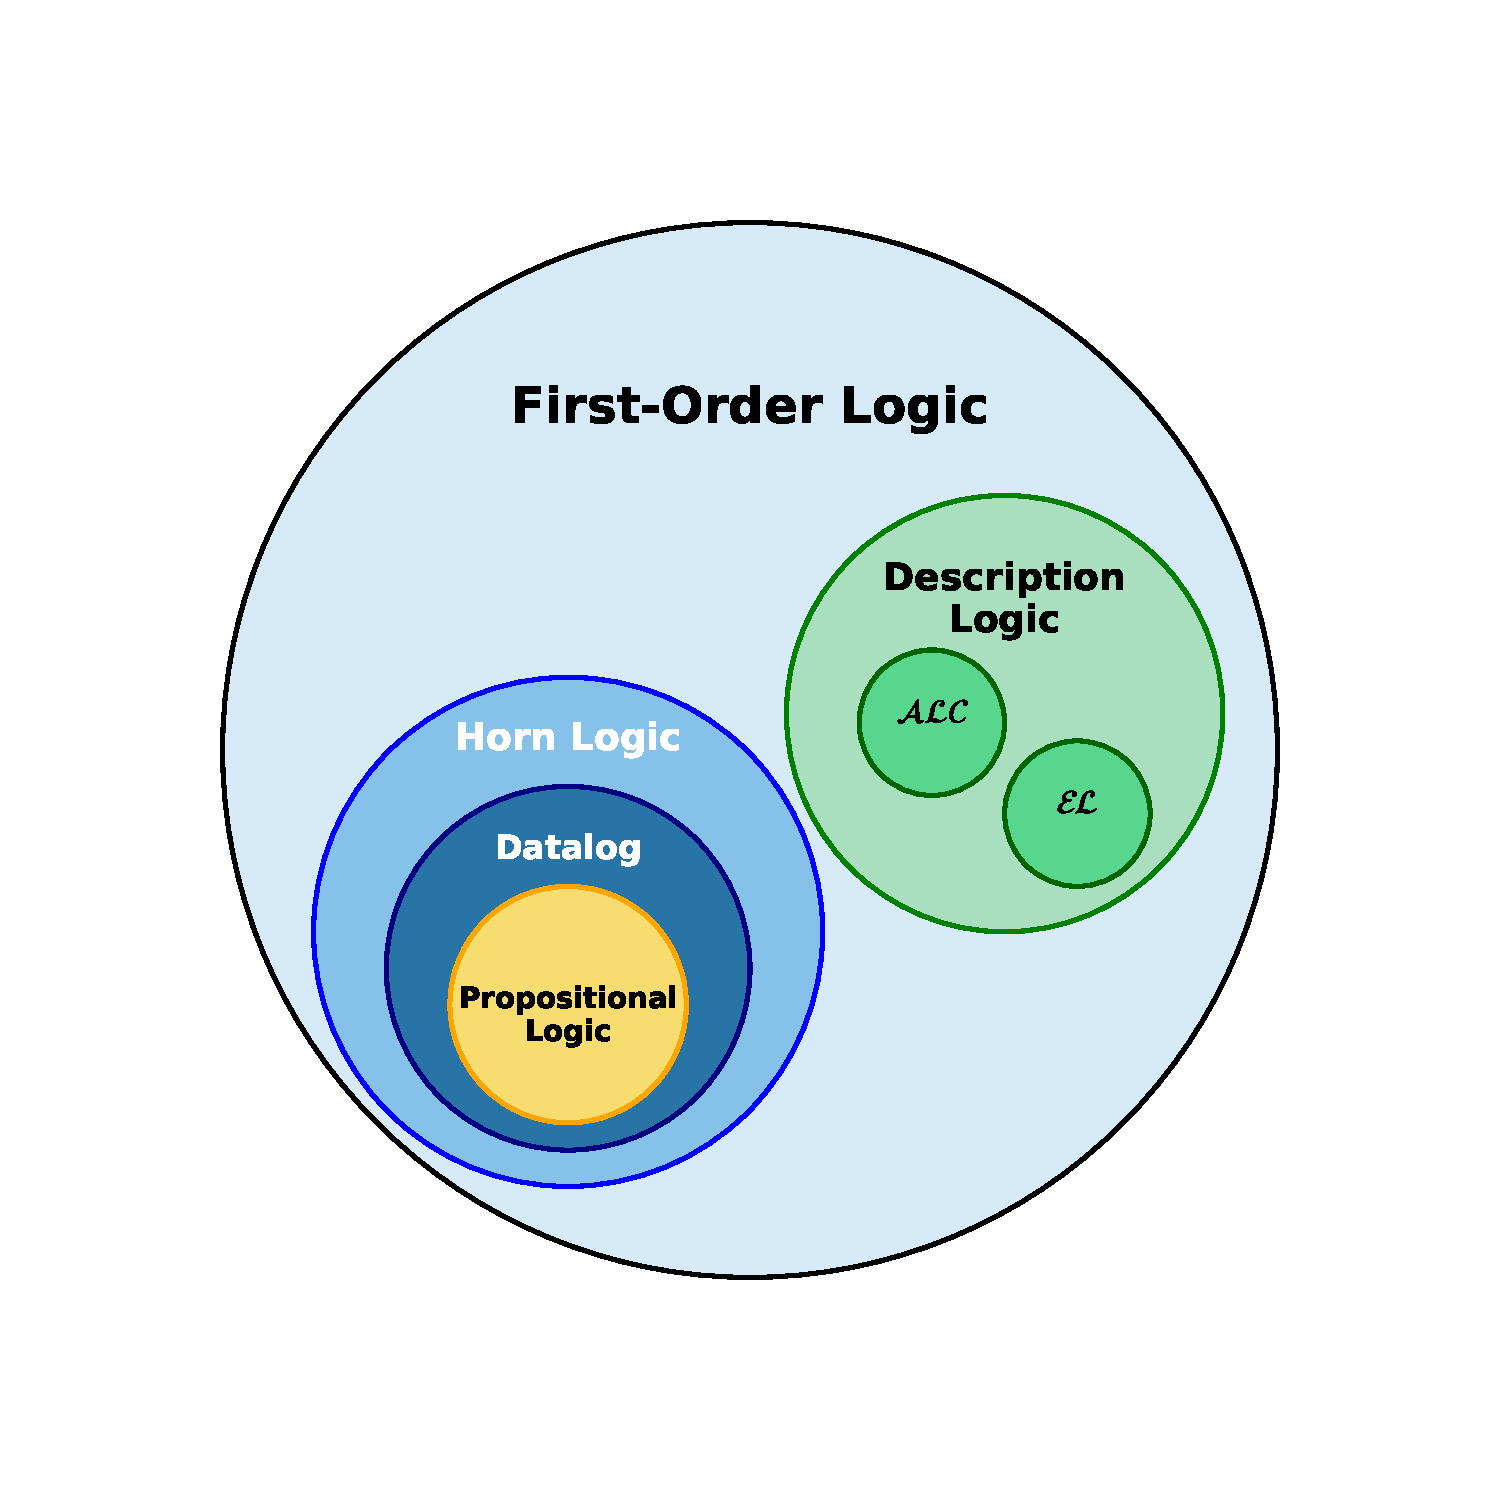
\includegraphics[width=0.58\textwidth]{figures/venn_diagram_logics}
    \caption[Venn diagram of different logic families]{
        %
        Venn diagram of different logic families, illustrating the trade-off between expressiveness and tractability.
        %
        \Gls{FOL} is the most expressive logic -- not the most expressive logic in general -- encompassing all others.
        %
        On the other hand, propositional logic is the least expressive, as it can only represent atomic propositions and their combinations.
        %
        All the other logics fall somewhere in between, with varying degrees of expressiveness and tractability.
    }
    \label{fig:venn-diagram-logics}
\end{SCfigure}

%
Tractability addresses the theoretical question of whether a logic reasoner can determine the truth of a given formula within feasible time and space bounds.
%
The answer is deeply tied to the specific reasoning algorithm and the logic's formal properties.
%
Depending on the features a logic provides -- such as quantifiers, function symbols, or recursive definitions -- it may be more or less expressive.
%
The higher the expressiveness, the more complex the problems that can be represented and reasoned about, but this also increases the computational burden.
%
This well-known phenomenon is often referred to as the expressiveness/tractability trade-off~\cite{DBLP:journals/jlp/CadoliS93,BRACHMAN2004327,DBLP:journals/ci/LevesqueB87}.
%
In practice, highly expressive logics make it easier for human users to model rich domains, often requiring fewer and more concise formulas.
%
However, this comes at the cost of automated inference, which may become computationally intractable, undecidable, or non-terminating in the general case.
%
To mitigate this issue, various fragments and extensions of \gls{FOL} have been identified, each providing different tradeoffs between what can be expressed and what can be decided efficiently.
%
\Cref{fig:venn-diagram-logics} illustrates the relationships among different logic families, highlighting the trade-off between expressiveness and tractability.


\subsection{\Glsentrylong{FOL}}\label{subsec:first-order-logic}
%
\Gls{FOL} is a general-purpose formalism that underpins most symbolic \gls{KR} systems.
%
It enables both human and computational agents to model entities and their interrelations through predicates and terms within a defined domain of discourse.
%
Its syntax comprises variables (quantified explicitly or implicitly), constants, function symbols, and predicate symbols, which are combined via logical operators such as conjunction (\(\wedge\)), disjunction (\(\vee\)), implication (\(\rightarrow\)), and equivalence (\(\leftrightarrow\)).
%
\Gls{FOL} allows for both \emph{extensional} and \emph{intensional} definitions.
%
Recursive intensional definitions, in particular, are powerful, enabling finite representations of infinite sets.
%
Despite its flexibility, \gls{FOL} is semi-decidable in general: there is no algorithm that can determine the truth of every \gls{FOL} formula in finite time, which limits its use in systems requiring guaranteed termination~\cite{DBLP:conf/dlog/2003handbook}.


\subsection{Horn logic}\label{subsec:horn-logic}
%
Horn logic is a significant subset of \gls{FOL}, offering a balanced trade-off between theoretical expressiveness and practical tractability~\cite{DBLP:journals/jcss/Makowsky87}.
%
It is built around the concept of \emph{Horn clauses}~\cite{DBLP:journals/jsyml/Horn51}, which are formulas in \gls{FOL} that exclude quantifiers and consist of a disjunction of predicates, with at most one non-negated literal.
%
Alternatively, a Horn clause can be expressed as an implication where the consequent is a single predicate and the antecedent is a conjunction of predicates: \(h \gets b_1, \dots, b_n\).
%
Here, \(\gets\) denotes logical implication (from right to left), commas represent logical conjunctions, and \(b_i\) as well as \(h\) are predicates of arbitrary arity, potentially containing \gls{FOL} terms such as variables, constants, or functions.

Horn clauses can be interpreted as \emph{if-then} rules written in reverse order, where only conjunctions of predicates are allowed in the antecedent.
%
In essence, Horn logic is a constrained subset of \gls{FOL} characterized by the following limitations:
%
\begin{inlinelist}
%
    \item formulas are reduced to clauses, containing only predicates, conjunctions, and a single implication operator;
    %
    \item operators such as \(\lor\), \(\leftrightarrow\), or \(\neg\) (negation) are not allowed;
    %
    \item variables are implicitly quantified; and
    %
    \item terms behave as they do in \gls{FOL}.
    %
\end{inlinelist}


\subsection{Datalog}\label{subsec:datalog}
%
Datalog is a declarative query language and a restricted subset of \gls{FOL}, designed for deductive databases and knowledge representation~\cite{DBLP:journals/jcss/AjtaiG94}.
%
It represents knowledge using function-free Horn clauses, as defined in \Cref{subsec:horn-logic}.
%
This restriction eliminates the use of function symbols, thereby forbidding structured terms such as recursive data structures.
%
As a result, Datalog is well-suited for applications requiring finite and decidable reasoning, as the absence of function symbols ensures termination of inference algorithms.
%
Similar to Horn logic, Datalog’s knowledge bases consist of sets of function-free Horn clauses, which are interpreted as rules and facts.
%
Rules in Datalog follow the form \(h \gets b_1, \dots, b_n\), where \(h\) is the head of the rule and \(b_1, \dots, b_n\) are the body predicates.
%
Unlike general \gls{FOL}, Datalog does not allow disjunctions, negations, or explicit quantifiers, as variables are implicitly universally quantified.
%
Datalog is widely used in areas such as \glspl{KG}, semantic web technologies, and database systems, where efficient reasoning over large datasets is required.
%
Its simplicity and computational efficiency make it a practical choice for symbolic \gls{AI} tasks that demand tractable reasoning.


\subsection{\Glsentrylong{DL}}\label{subsec:dl}
%
\Gls{DL} are a family of subsets of \gls{FOL}, typically involving limited or no quantifiers, no structured terms, and no \textit{n}-ary predicates where \(n \geq 3\)~\cite{DBLP:books/daglib/0041477}.
%
In essence, \gls{DL} represents knowledge using constants and variables, along with atomic, unary, and binary predicates.


The differences among specific variants of \gls{DL} lie in the set of supported logical connectives and whether negation is allowed.
%
The wide variety of \gls{DL} stems from the well-known trade-off between expressiveness and tractability.
%
Depending on the application, one may prefer a more expressive \gls{DL} variant, which offers richer features at the cost of reduced tractability or even decidability of algorithms manipulating the knowledge, or vice versa.


In \gls{DL}, it is common practice to use specific terminology for different elements of knowledge representation:
%
\begin{itemize}
    %
    \item Constant terms are referred to as \textit{individuals}, as each constant represents a single entity within a domain.
    %
    \item Unary predicates are called \textit{classes} or \textit{concepts}, grouping sets of individuals for which the predicate holds true.
    %
    \item Binary predicates are referred to as \textit{properties} or \textit{roles}, connecting pairs of individuals.
    %
\end{itemize}
%

Using this nomenclature, knowledge in \gls{DL} can be represented by associating entities with constants (e.g., URLs) and defining concepts and properties accordingly.
%
Binary predicates are particularly significant as they enable the connection of pairs of entities.
%
This is typically achieved through subject–predicate–object triplets, represented as ground binary predicates of the form \(\langle a \, f \, b\rangle\) or \(f(a, b)\), where \(a\) is the subject, \(f\) is the predicate, and \(b\) is the object.

Collections of such triplets form \glspl{KG}, which are directed graphs where vertices represent individuals and arcs represent binary properties connecting these individuals.
%
\glspl{KG} may explicitly or implicitly instantiate a specific ontology, which is a formal description of classes characterizing a domain, their relationships (e.g., inclusion, exclusion, intersection, equivalence), and the properties they must or must not include.


\glspl{DL} are widely used in applications such as semantic web~\cite{DBLP:conf/coopis/GangemiM03} and ontology engineering~\cite{DBLP:books/ios/HGJKP2016}, where efficient reasoning and knowledge representation are essential.
%
Their ability to balance expressiveness and computational efficiency makes them a cornerstone of symbolic reasoning systems.


\subsection{Ontologies and \glsentrylong{KG}}\label{subsec:ontologies-and-kg}
%
An ontology is a formal and explicit specification of a shared conceptualisation of a domain~\cite{DBLP:books/daglib/p/Grimm10}.
%
It provides a structured vocabulary to describe the entities relevant in that domain, along with their attributes and the relationships among them.
%
This organisation enables both human understanding and machine-based reasoning.

Ontologies are typically expressed using \glspl{DL}, a family of logic-based formalisms for knowledge representation.
%
\Glspl{DL} define three main components:
%
\begin{inlinelist}
    %
    \item\emph{concepts} (or \emph{classes}), which group entities sharing similar features;
    %
    \item\emph{individuals} (or \emph{instances}), which are the concrete elements of the domain;
    %
    \item\emph{roles} (or \emph{properties}), which describe binary relationships between individuals.
    %
\end{inlinelist}
%
Different \glspl{DL} vary in their expressive power: for example, \gls{EL} supports only conjunction and existential quantification to ensure efficient reasoning, while more expressive DLs like \gls{ALC} allow for full Boolean operators and universal quantification.

Concepts are typically denoted using capital italic letters, such as $\mathit{Animal}$ or $\mathit{Cat}$.
%
These can be combined using logical constructors like intersection ($\sqcap$), union ($\sqcup$), or negation ($\lnot$) to form more complex classes.
%
A statement like $\mathit{Cat} \sqsubseteq \mathit{Animal}$ expresses that all cats are animals.

Individuals are constants representing specific entities in the domain and are usually written in monospaced lowercase, for example \texttt{tom}.
%
Membership of an individual in a concept is denoted using the ``is-a'' relation, written as \texttt{tom}~:~$\mathit{Cat}$, meaning ``Tom is a cat.''
%
Each individual may belong to multiple concepts.

Roles represent binary relations between individuals and are written in lowercase sans-serif font, such as \textsf{eats}.
%
They connect pairs of individuals, and their domain and range can be restricted using expressions such as $\textsf{eats} \sqsubseteq \mathit{Animal} \times \mathit{Edible}$.
%
Assertions like $\textsf{eats}(\texttt{tom}, \texttt{mouse})$ state that Tom eats the mouse.

The subsumption relation ($\sqsubseteq$) is used to express inclusion between concepts or roles.
%
For instance, $\mathit{Cat} \sqsubseteq \mathit{Animal}$ means that every cat is also an animal, and $\textsf{predatorOf} \sqsubseteq \textsf{eats}$ means that every predator-prey relationship implies eating.
%
Special concepts such as $\top$ and $\bot$ are used to denote the most general and the most specific concepts, respectively.

Collections of such axioms form an ontology.
%
\Gls{TBOX} define concepts and roles and their interrelations, while \gls{ABOX} specify which individuals belong to which concepts or are related via which roles.

\Glspl{KG} also provide a structured way to represent knowledge as graphs.
%
They consist of triplets (or \emph{facts}) of the form $(s, p, o)$, where $s$ is the subject, $p$ is the predicate (or property), and $o$ is the object.
%
These triplets form a directed graph where nodes represent individuals and edges represent relationships.

Unlike ontologies, KGs do not necessarily impose formal constraints on the structure or semantics of the triplets.
%
This flexibility allows for representing heterogeneous and incomplete data.
%
However, some \glspl{KG} are explicitly grounded in an ontology, and may follow its vocabulary and logical constraints.

In summary, ontologies and knowledge graphs both aim to formally capture structured knowledge.
%
Ontologies provide formal semantics and enable logical reasoning, while knowledge graphs emphasise scalability and flexibility in representing factual data.


\subsection{Propositional Logic}\label{subsec:propositional-logic}
%
Propositional logic is a restricted subset of \gls{FOL} in which quantifiers, terms, and non-atomic predicates are absent.  
%
Its language consists solely of atomic propositions—also called 0-ary predicates—combined using standard logical connectives such as conjunction ($\land$), disjunction ($\lor$), negation ($\lnot$), and implication ($\rightarrow$).  
%
Each proposition can be interpreted as a Boolean variable that takes a truth value in \{\texttt{true}, \texttt{false}\}.  
%
The semantics of propositional logic aligns with Boolean algebra, making it straightforward to evaluate the truth of a formula given the truth values of its atomic components.

For example, a propositional formula such as $p \land \lnot q \rightarrow r$ can be interpreted as follows:  
%
$p$ might stand for the proposition ``it is raining,'' $q$ for ``there is a roof,'' and $r$ for ``the floor is wet.''  
%
In this case, the formula asserts that if it is raining and there is no roof, then the floor will be wet.

Compared to \gls{FOL}, propositional logic is significantly less expressive.  
%
The absence of quantifiers means that general statements over a domain cannot be made.  
%
Similarly, the lack of terms prevents direct reference to entities in the domain.  
%
As a consequence, each relevant aspect of a scenario must be explicitly encoded as an individual proposition.

This limitation in expressiveness has important computational implications.  
%
In particular, determining the satisfiability of a propositional formula is a decidable problem.  
%
This makes propositional logic attractive in scenarios where tractable reasoning is required.

Despite its apparent simplicity, propositional logic can model a surprising range of situations.  
%
Expressions involving numerical constants, variables, and comparisons (e.g., $x > 5$ or $y = 3$) can be encoded propositionally by introducing a distinct Boolean variable for each comparison.  
%
This reduction allows the use of propositional logic in settings where the original problem does not explicitly involve logical variables or quantifiers, but can be decomposed into atomic truth conditions.


\subsection{Limits of symbolic \Gls{AI}}\label{subsec:limits-of-symbolic-ai}
%



\section{Sub-symbolic \Gls{AI}}\label{sec:sub-symbolic-ai}
%
Sub-symbolic \gls{AI} encompasses a wide range of techniques that rely on numerical representations.
%
Contributions come from varius fields, including \gls{ML}, statistical learning, and data mining.
%
The huge number of approaches is also motivated by the well known \gls{NFL} theorem~\cite{DBLP:journals/tec/DolpertM97} that states that no single learning algorithm can outperform all others across all possible tasks.
%
The most common predictor families are linear models, \glspl{DT}, \glspl{RF}, \glspl{SVM}, \glspl{NN} (including \glspl{LLM}), and many others.


\paragraph{Predictive performance vs. interpretability}
%
\begin{figure}[h]
    \centering
    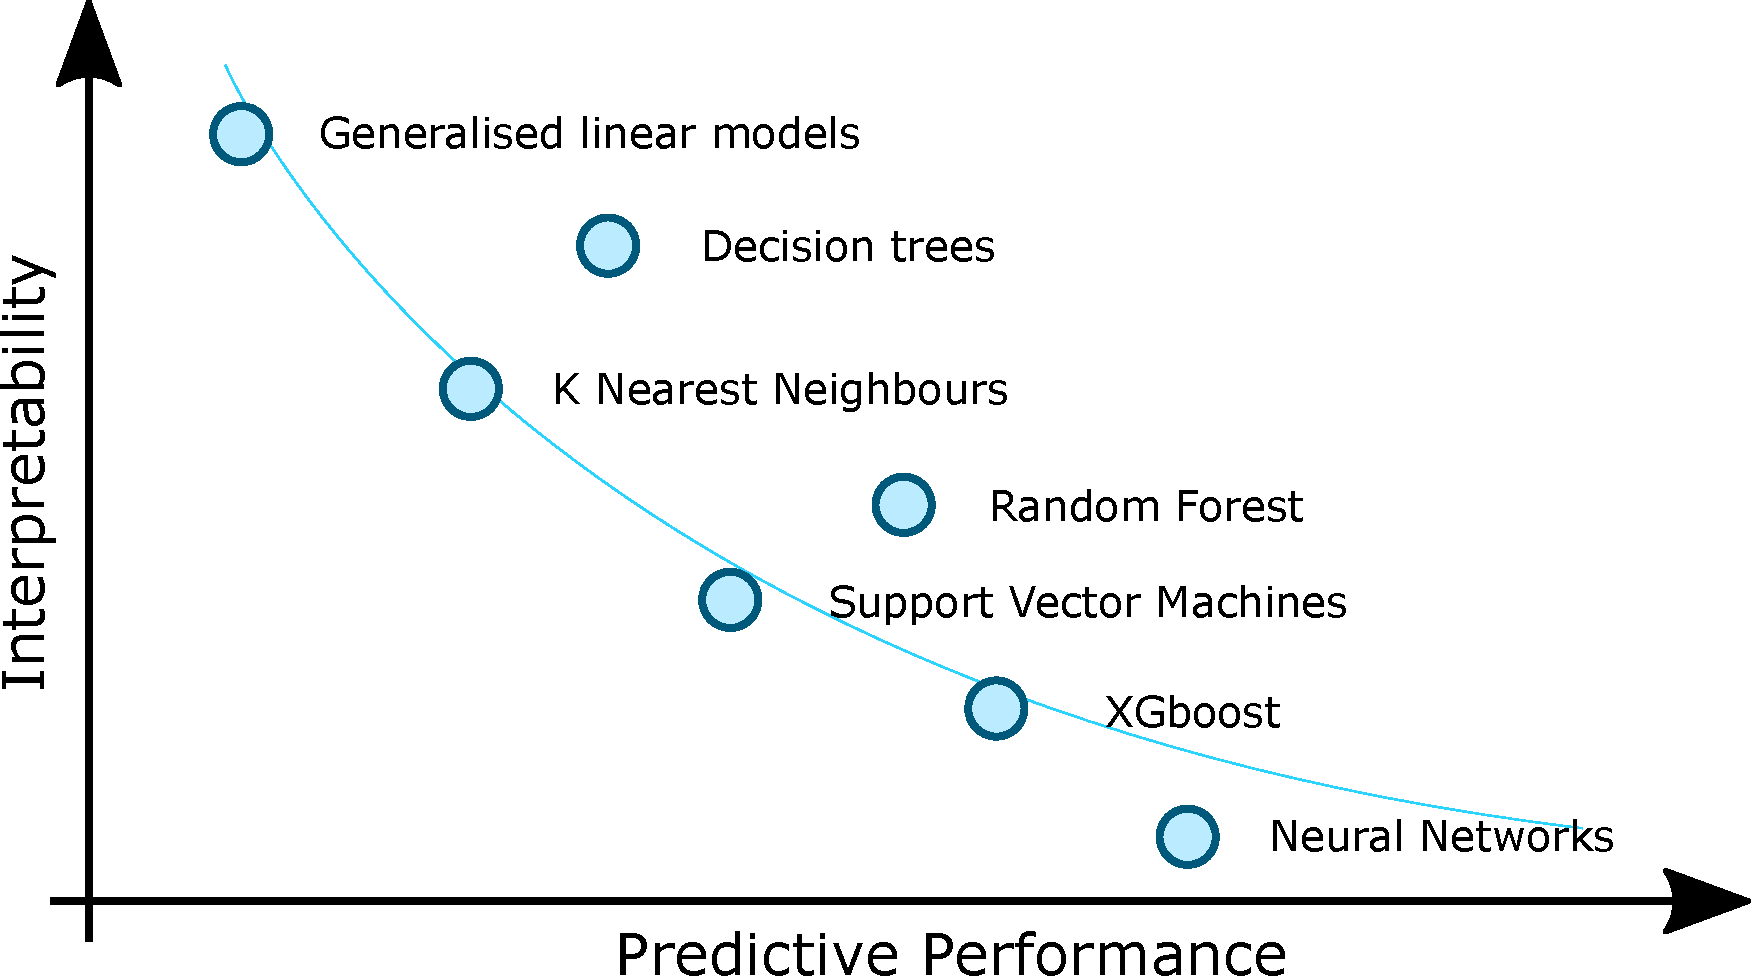
\includegraphics[width=0.9\textwidth]{figures/interpretability-performance-tradeoff}
    \caption[Performance vs. interpretability trade-off]{
        %
        Trade-off between predictive performance and interpretability in common sub-symbolic predictors.
        %
        The figure illustrates how different predictor families balance these two aspects, with simpler models being more interpretable but potentially less accurate.
        %
    }
    \label{fig:performance-vs-interpretability}
\end{figure}
%
The \emph{complexity} of a sub-symbolic predictor can vary significantly.
%
By complexity we mean the overall structure of the model, including the number of parameters, the operations that are performed, and possibly the way the model is trained.
%
\Glspl{DT}, for example, are relatively simple models that can be easily interpreted by humans.
%
The downside of \glspl{DT} is that they make predictions by linearly partitioning the input space, which can lead to poor generalisation on unseen data.
%
On the other hand, \glspl{NN} can be extremely complex, with millions of parameters and intricate architectures that are difficult to interpret.
%
However, \glspl{NN} can capture highly non-linear relationships in the data, often leading to superior predictive performance compared to simpler models.
%
The definition of interpretability is not univocal, and it lacks measures that are widely accepted~\cite{DBLP:journals/natmi/Rudin19}.
%
Despite that, \Cref{fig:performance-vs-interpretability} illustrates in an informal way the trade-off between predictive performance and interpretability in sub-symbolic predictors.


\subsection{\Glsentrylongpl{DT}}\label{subsec:decision-trees}

\subsection{\Glsentrylongpl{RF}}\label{subsec:random-forests}

\subsection{\Glsentrylongpl{SVM}}\label{subsec:svm}

\subsection{\Glsentrylongpl{NN}}\label{subsec:neural-networks}

\subsection{Limits of sub-symbolic \Gls{AI}}\label{subsec:limits-of-sub-symbolic-ai}
%! Author = matteomagnini
%! Date = 05/03/25

%----------------------------------------------------------------------------------------
\chapter{Neuro-symbolic AI}
\label{ch:nesy-ai}
\minitoc
%----------------------------------------------------------------------------------------

\section[Symbolic knowledge injection]{\Glsentrylong{SKI}}\label{sec:ski}
%
\Gls{SKI} is a wide sub-field of \gls{NeSy}, which encompasses all the methods that in some way \emph{inject} symbolic knowledge into sub-symbolic predictors.
%
More precisely, we define \gls{SKI} as:
%
\begin{definition}[\gls{SKI}]
    \label{def:ski}
    any algorithmic procedure affecting how sub-symbolic predictors draw their inferences in such a way that predictions are either \textbf{computed} as a function of, or \textbf{made consistent} with, some given symbolic knowledge~\cite{DBLP:journals/csur/CiattoSAMO24}.
\end{definition}
%
We adopt this broad definition because the amount of works in the literature is vast and varied, furthermore the contributions come from different communities (e.g., \gls{ML}, \gls{AI}, \gls{NLP}, \gls{XAI}, logics, etc.), and they often use different terminologies.


\subsection{Motivations and goals}\label{subsec:ski-motivations-and-goals}
%
\Gls{SKI} can be used for several reasons, such as:
%
\begin{inlinelist}
    %
    \item \label{itm:prediction}\emph{improving the model's predictive performance}, by leveraging symbolic knowledge to guide their learning or inference;
    %
    \item \label{itm:interpretability}\emph{improving the model's interpretability}, by making their predictions consistent with symbolic knowledge;
    %
    \item \label{itm:robustness}\emph{increase the robustness} of sub-symbolic predictors, by making them less sensitive to data perturbations (e.g., noise, data scarcity, etc.);
    %
    \item \label{itm:complexity}\emph{reduce the model complexity} of the models, by shaping their structure or by constraining their parameters;
    %
    \item and possibly many more.
    %
\end{inlinelist}


\Cref{itm:prediction} is one of the most common motivations for \gls{SKI}.
%
The idea is simple: if there is already some (symbolic) knowledge about a particular domain or task, then it is reasonable to expect that the predictor can benefit from it.
%
In this way the model learns both from the data -- inductively -- and from the symbolic knowledge---mimicking deductive reasoning.


Another common reason to use \gls{SKI} is to increase the \emph{interpretability} of the model, as stated in \Cref{itm:interpretability}.
%
In the context of \gls{XAI}, this is usually referred as \gls{XAI} \emph{by design} (\Cref{par:xai-by-design}).
%
The intuition is simple: the model is made to be consistent -- up to a certain extent -- with the symbolic knowledge, which is usually more interpretable than the model itself.
%
This can be done in two ways: either by using \emph{symbols as constraints} or by \emph{transparent box design}.
%
More details about these two approaches are provided in \Cref{subsec:learning} and \Cref{subsec:structuring}, respectively.


Predictive performances and \gls{XAI} are the main motivations for \gls{SKI}, but not the only ones.
%
The \emph{robustness} (\Cref{itm:robustness}) of a predictive model is another important challenge~\cite{DBLP:conf/eccv/LiuCZH18}, and it relates to predictors' ability to maintain performance despite the presence of input perturbations.
%
A metric of robustness in the context of \gls{SKI} is defined in the work ``An Empirical Study on the Robustness of Knowledge Injection Techniques Against Data Degradation''~\cite{DBLP:conf/woa/RafanelliMACO24}.
%
The content of the paper is presented in~\Cref{subsec:empirical-study-on-the-robustness-of-ski-methods}.
%
Along with robustness, there are other metrics -- often neglected -- that play a crucial role in the design of intelligent systems, such as \emph{memory footprint} (\Cref{itm:complexity}), \emph{latency}, data efficiency, and so on.
%
These \gls{QoS} metrics are presented in the work ``Symbolic Knowledge Injection Meets Intelligent Agents: QoS metrics and experiments''~\cite{DBLP:journals/aamas/AgiolloRMCO23}, which is discussed in~\Cref{subsec:ski-meets-intelligent-agents}.


\subsection{What to inject}\label{subsec:what-to-inject}
%
\begin{SCfigure}
    \centering
    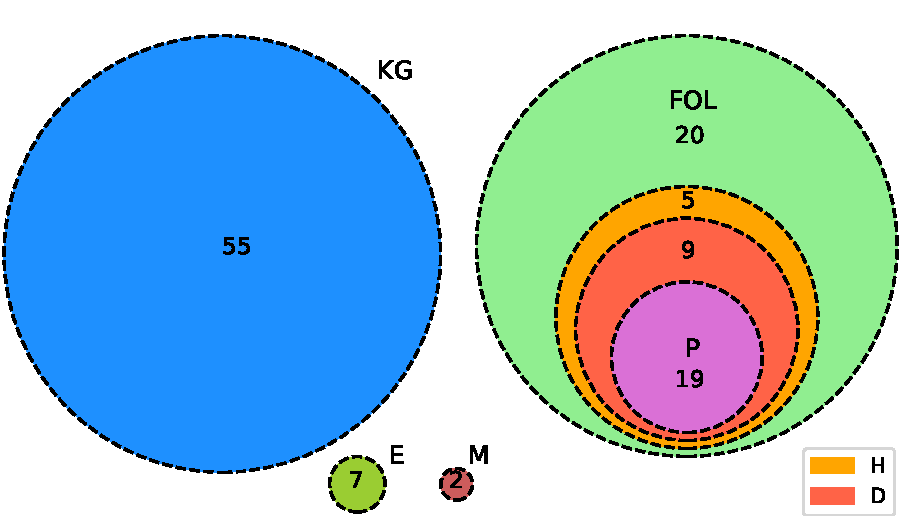
\includegraphics[width=.4\linewidth]{figures/ski-logic}
    \caption[Venn diagram categorising SKI methods]{
        Venn diagram categorising SKI methods w.r.t.\ the \emph{input knowledge} type: knowledge graphs (KG), propositional logic (P), first-order logic (FOL), expert knowledge (E), Datalog (D), Horn logic (H), or modal logic (M).
        %
        The image is taken from~\cite{DBLP:journals/csur/CiattoSAMO24} and it refers to 117 surveyed \gls{SKI} methods.
    }
    \label{fig:pie-ski-logic}
\end{SCfigure}

%
A key distinction in \gls{SKI} methods lies in whether the chosen formalism is \emph{machine interpretable}, \emph{human interpretable}, or both.
%
\Gls{SKI} methods can be categorized into two primary groups based on the formalism used to represent input knowledge~\cite{DBLP:journals/csur/CiattoSAMO24}:
%
\begin{itemize}
    \item \textbf{Logic formulas or \glspl{KB}:} These adhere to \gls{FOL} or its subsets, making them interpretable by both humans and machines.
    %
    The sub-categories, ordered by decreasing expressiveness, include:
    %
    \begin{itemize}
        %
        \item \emph{\gls{FOL} formulas:} These encompass recursive terms, variables, predicates of any arity, and various logic connectives, potentially expressing definitions.
        %
        \item \emph{Horn logic:} Often referred to as Prolog-like logic, this formalism consists of head–body rules involving predicates and terms of any kind.
        %
        \item \emph{Datalog:} A restricted subset of Horn logic that excludes recursive terms, allowing only constants or variables as terms.
        %
        \item \emph{Modal logics:} These extend the above logics with modal operators (e.g., \(\square\) and \(\lozenge\)), which express modalities such as necessity or possibility.
        %
        \item \emph{Knowledge graphs:} A practical application of description logics designed to represent entity–relation graphs.
        %
        \item \emph{Propositional logic:} This involves Boolean variables and logical connectives, offering a simpler yet effective formalism.
    \end{itemize}
    %
    \item \textbf{Expert knowledge:} This category includes human-interpretable knowledge that is not inherently machine-readable.
    %
    Examples include physics equations, syntactical rules, or domain-specific expertise.
    %
    Since expert knowledge is not directly machine interpretable, it often requires transformation into tensorial form through data generation, a process that typically involves human engineers and can be labor-intensive.
\end{itemize}
%
\Cref{fig:pie-ski-logic} illustrates the distribution of surveyed \gls{SKI} methods based on their formalism of choice.
%
\Glspl{KG} emerge as the most prevalent category, representing nearly half of the surveyed methods.
%
In contrast, modal logics constitute the smallest group.
%
Methods based on \gls{FOL} or its subsets (excluding \glspl{KG}) form another significant cluster, with propositional logic being particularly prominent due to its relative simplicity and widespread use.
%
The specific logic formalism employed in the surveyed papers is reported where available.
%
However, this information is rarely explicitly stated by the authors.
%
Instead, the logic is often inferred from the constraints and descriptions provided in the respective works.

Practical examples of symbolic knowledge that can be injected into sub-symbolic predictors are the public health guidelines on type-2 diabetes of the National Institute of Diabetes and Digestive and Kidney Diseases\footnote{\url{https://www.niddk.nih.gov/health-information/diabetes/}}.
%
These guidelines have been encoded into logic formulas~\cite{DBLP:conf/pkdd/KunapuliBSMS10} and used in works related to \gls{SKI}~\cite{Magnini-telmed2025}.
%
The first guideline state that if a patient has a glucose value greater or equal to 125 mg/dL and a \gls{BMI} greater or equal to 30, then the patient is considered diabetic.
%
The second one says that if a patient has a glucose value lower or equal to 100 mg/dL and a \gls{BMI} lower or equal to 25, then the patient is considered non-diabetic.
%
In \gls{FOL}, the first statement can be encoded as:
%
\begin{equation}\label{eq:rule-diabetic}
  \forall x . ( \text{glucose}(x) \geq 125 \land \text{bmi}(x) \geq 30 \rightarrow \text{Diabetic}(x))
\end{equation}
%
whereas the second statement can be encoded as:
%
\begin{equation}\label{eq:rule-not-diabetic}
  \forall x . ( \text{glucose}(x) \leq 100 \land \text{bmi}(x) \leq 25 \rightarrow \neg \text{Diabetic}(x))
\end{equation}


\subsection{How to inject}\label{subsec:how-to-inject}
%



\subsection{Structuring}\label{subsec:structuring}

\subsection{Learning}\label{subsec:learning}

\subsection{Embedding}\label{subsec:ski-embedding}

\subsection[Limitations and challenges of SKI]{Limitations and challenges of \Gls{SKI}}\label{subsec:limitations-and-challenges-of-ski}

\section[Symbolic knowledge extraction]{\Glsentrylong{SKE}}\label{sec:ske}

\subsection{Motivations and goals}\label{subsec:ske-motivations-and-goals}

\subsection{How to extract}\label{subsec:how-to-extract}

\subsection[Decompositional SKE]{Decompositional \Gls{SKE}}\label{subsec:decompositional-ske}

\subsection[Pedagocial SKE]{Pedagocial \Gls{SKE}}\label{subsec:pedagogical-ske}

\subsection{Local explanations}\label{subsec:local-explanations}

\subsection{Global explanations}\label{subsec:global-explanations}

\subsection[Limitations and challenges of SKE]{Limitations and challenges of \Gls{SKE}}\label{subsec:limitations-and-challenges-of-ske}
%! Author = matteomagnini
%! Date = 05/03/25

%----------------------------------------------------------------------------------------
\chapter{Large Language Models}
\label{ch:llm}
\minitoc
%----------------------------------------------------------------------------------------

\section{Architectures}\label{sec:llm-architectures}

\subsection{Transformer}\label{subsec:transformer}

\subsection{Attention}\label{subsec:attention}

\section{Fine-tuning}\label{sec:llm-fine-tuning}

\section{\Glsentrylong{RAG}}\label{sec:rag}

\subsection{Embedding}\label{subsec:rag-embedding}

\subsection{Retrieval}\label{subsec:retrieval}

\section{Limitations and challenges}\label{sec:limitations-and-challenges}

\subsection{Resources}\label{subsec:resources}

\subsection{Data and privacy}\label{subsec:data-and-privacy}

\subsection{Hallucinations}\label{subsec:hallucinations}

\subsection{Stochastic parrot or something more?}\label{subsec:stochastic-parrot-or-something-more}
\printbibliography[title=References,heading=bibintoc]
\end{refsection}

%----------------------------------------------------------------------------------------
%-------------------------------------- PART II -----------------------------------------
%----------------------------------------------------------------------------------------

\part{Engineering of \ac{SKI} \& \ac{SKE}}
\label{part:engineering-of-ski-ske}

\begin{refsection}
%! Author = matteomagnini
%! Date = 05/03/25

%----------------------------------------------------------------------------------------
\chapter{Common patterns}
\label{ch:common-patterns}
%----------------------------------------------------------------------------------------

\section{Knowledge representation}\label{sec:knowledge-representation}

\subsection{Logic rules}\label{subsec:logic-rules}

\subsection{\Aclp{KG}}\label{subsec:kg}

\subsection{Free text}\label{subsec:free-text}

\section{From symbolic to sub-symbolic}\label{sec:from-symbolic-to-sub-symbolic}

\subsection{Fuzzyfication}\label{subsec:fuzzyfication}

\subsection{Delegation}\label{subsec:delegation}

\section{From sub-symbolic to symbolic}\label{sec:from-sub-symbolic-to-symbolic}

\subsection{Surrogate models}\label{subsec:surrogate-models}

\subsection{De-fuzzyfication}\label{subsec:unfuzzyfication}

%! Author = matteomagnini
%! Date = 05/03/25

%----------------------------------------------------------------------------------------
\chapter[Platform for symbolic knowledge injection]{\Glsentrylong{PSyKI}}
\label{ch:psyki}
\minitoc
%----------------------------------------------------------------------------------------

In this chapter, we present the \Gls{PSyKI} platform, which is a framework for \gls{SKI} methods.
%
\Gls{PSyKI} provides a unified way to implement \gls{SKI} methods, aiming to facilitate the development and comparison of different approaches.
%
It also provides a set of tools to evaluate the performance of \gls{SKI} methods, including metrics for measuring the quality of the injected knowledge and the performance of the resulting models.
%
In \Cref{sec:psyki}, we present the work ``\emph{On the Design of PSyKI: A Platform for Symbolic Knowledge Injection into Sub-symbolic Predictors}''~\cite{DBLP:conf/atal/MagniniCO22}, which describes the design and implementation of \gls{PSyKI}.
%
Then, in \Cref{sec:qos}, we present respectively two works that study the quality of service of \gls{SKI} methods:
%
in \Cref{sec:ski-meets-intelligent-agents} the paper ``\emph{Symbolic Knowledge Injection Meets Intelligent Agents}''~\cite{DBLP:journals/aamas/AgiolloRMCO23},
%
which introduces metrics for evaluating the performance of \gls{SKI} methods in the context of intelligent agents,
%
and in \Cref{sec:empirical-study-on-the-robustness-of-ski-methods} the paper ``\emph{An Empirical Study on the Robustness of Symbolic Knowledge Injection Techniques Against Data Degradation}''~\cite{DBLP:conf/woa/RafanelliMACO24},
%
which studies the robustness of \gls{SKI} methods against data degradation.


\section{PSyKI}\label{sec:psyki}
%
\Gls{PSyKI} is a (Python) platform for the development and evaluation of \gls{SKI} methods.
%
It is designed to provide a unified framework for implementing \gls{SKI} methods, allowing researchers and practitioners to easily develop, test, and compare different approaches.
%
In the following, we present a summary of the work ``\emph{On the Design of PSyKI: A Platform for Symbolic Knowledge Injection into Sub-symbolic Predictors}''~\cite{DBLP:conf/atal/MagniniCO22}, presented at the 4th International Workshop on EXplainable, Trustworthy, and Responsible AI and Multi-Agent Systems (EXTRAAMAS 2022)\footnote{\url{https://extraamas.ehealth.hevs.ch/archive.html}}.
%
The library is public available on GitLab and PyPi\footnote{\url{https://gitlab.com/psykei/psyki-python} and \url{https://pypi.org/project/psyki/}}.


\subsection{Motivations}\label{subsec:psyki-motivations}
%
This work is motivated by the need to address the common challenges that affect \gls{SKI} methods (see \Cref{subsec:limitations-and-challenges-of-ski}).
%
In particular, we want to address the following points:
%
\begin{inlinelist}
    \item \emph{lack of generality}, by providing the proper tools to automatically translate symbolic knowledge of arbitrary domains into a format suitable for injection into sub-symbolic predictors,
    %
    \item \emph{lack of reproducibility}, by providing a unified framework for implementing \gls{SKI} methods, allowing researchers to easily develop, test, and compare different approaches, and
    %
    \item \emph{lack of availability}, by encouraging the development of reusable software libraries for \gls{SKI} methods.
    %
\end{inlinelist}
%
Concerning the last point mentioned in \Cref{subsec:limitations-and-challenges-of-ski}, we identified in the logic language of stratified Datalog with negation a suitable candidate for the symbolic knowledge representation.
%
It is expressive enough to represent a wide range of symbolic knowledge, while being simple enough to be easily translated into a format suitable for injection into sub-symbolic predictors.


\subsection{Design}\label{subsec:design-and-implementation}
%
\begin{figure}
    \centering
    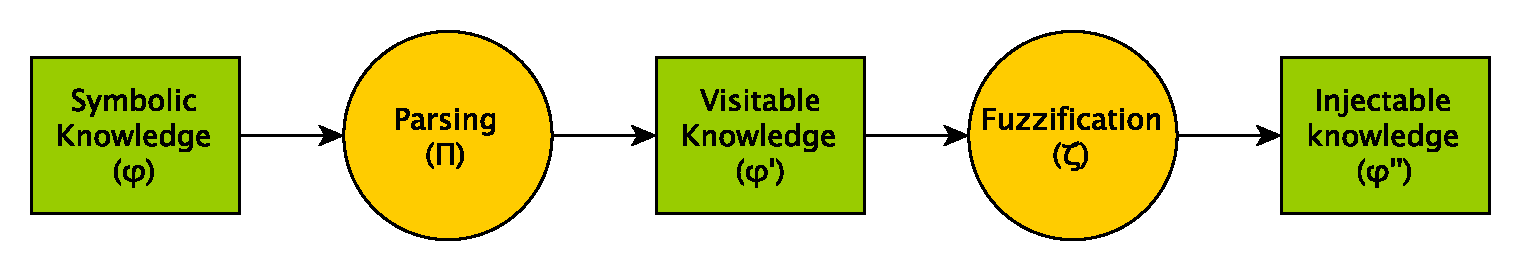
\includegraphics[width=\textwidth]{figures/knowledge-workflow-psyki}
    \caption[Symbolic knowledge transformation in PSyKI]{
        General workflow of symbolic knowledge transformation in \Gls{PSyKI}.
        The symbolic knowledge ($\phi$), typically expressed as logical formulas, is first parsed into a visitable form ($\phi'$), and then fuzzified into a machine-injectable representation ($\phi''$).
    }
    \label{fig:knowledge-workflow-psyki}
\end{figure}
%
All symbolic knowledge injection (\gls{SKI}) methods implemented in \gls{PSyKI} share a common transformation pipeline, illustrated in \Cref{fig:knowledge-workflow-psyki}.
%
Symbolic knowledge \(\phi\) cannot usually be injected directly into a sub-symbolic predictor.
%
Instead, it undergoes a two-step transformation:
%
\begin{inlinelist}
    %
    \item \emph{Parsing} (\(\Pi\)): the knowledge is converted into a visitable data structure, such as an \gls{AST} in the case of logic formulas, resulting in \(\phi'\);
    %
    \item \emph{Fuzzification} (\(\zeta\)): the parsed representation is transformed into a sub-symbolic form \(\phi''\), suitable for injection.
    %
\end{inlinelist}
%
Fuzzification plays a key role in bridging the symbolic and sub-symbolic domains.
%
It translates crisp Boolean logic into a form compatible with sub-symbolic models, often by relaxing discrete truth values into continuous-valued functions or generating neural components such as layers or entire \glspl{NN}.

\begin{figure}
    \centering
    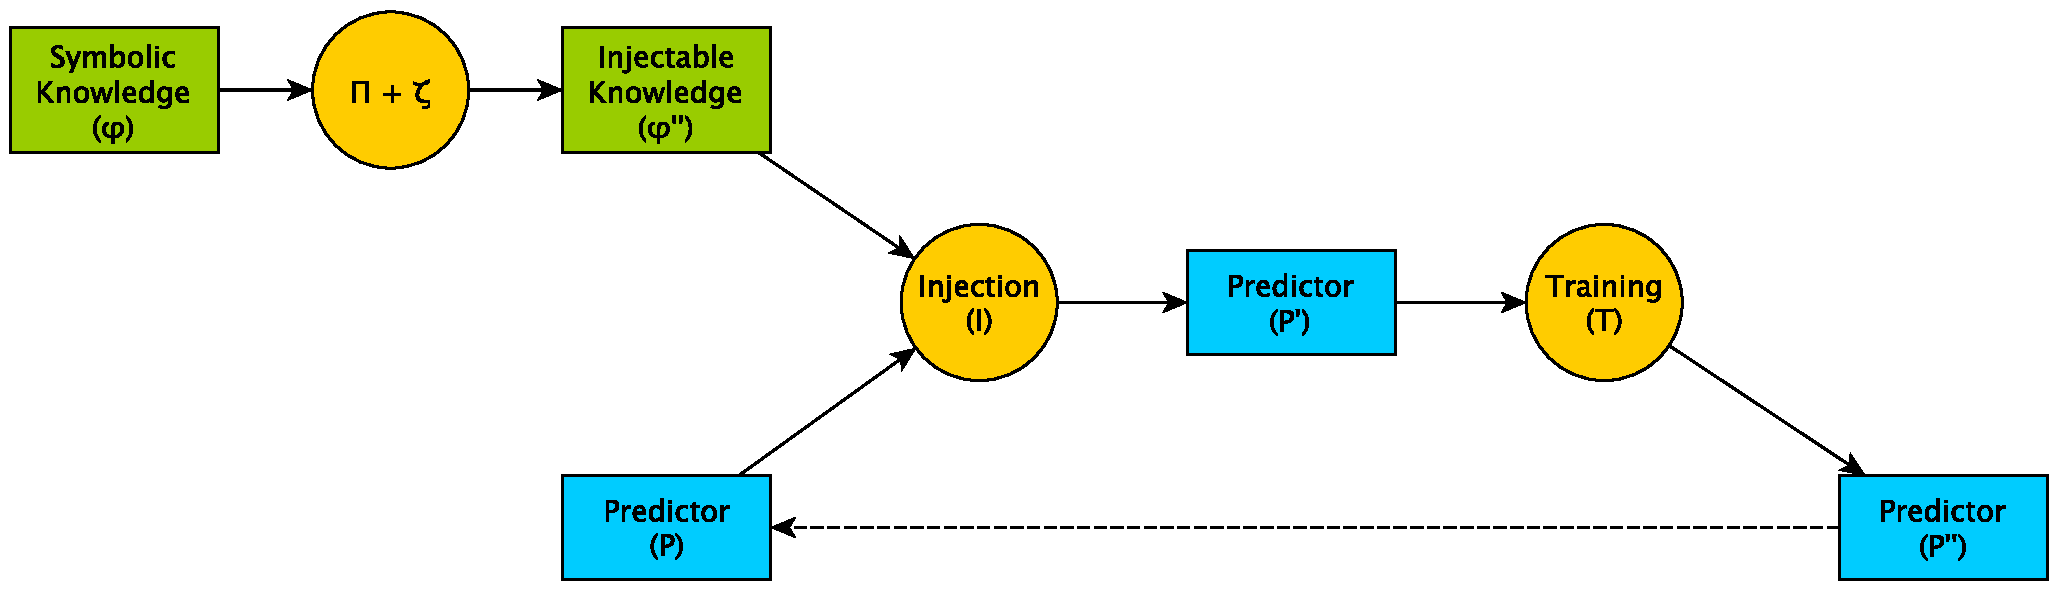
\includegraphics[width=\textwidth]{figures/psyki-workflow}
    \caption[General workflow of PSyKI]{
        Complete workflow of structuring and guided learning \gls{SKI} methods in \Gls{PSyKI}.
        The symbolic knowledge is transformed and injected into the sub-symbolic predictor, which is then trained on data.
    }
    \label{fig:psyki-workflow}
\end{figure}
%
\Cref{fig:psyki-workflow} shows the overall injection process in \gls{PSyKI}, including both the transformation of the symbolic knowledge and its integration into the learning system.
%
After the transformation phase, the different \gls{SKI} methods diverge:
%
\begin{inlinelist}
    %
    \item \emph{Structuring} and \emph{guided learning} inject \(\phi''\) directly into the architecture or training process of the predictor;
    %
    \item \emph{Embedding}-based methods use symbolic knowledge to enrich or generate the input data, so they are not directly represented in \Cref{fig:psyki-workflow}.
    %
\end{inlinelist}

\Gls{PSyKI} supports all three approaches, although it is primarily designed for \emph{structuring} and \emph{guided learning}, where the injection occurs directly into the predictor.
%
In general, \gls{SKI} algorithms operate on a predictor \(P\) and symbolic knowledge \(\phi\), producing a new predictor \(P'\) as output.
%
This modified predictor is then trained on data, resulting in a final model \(P''\), which can be reused in further iterations with different knowledge or injection strategies.


\paragraph{Architecture}\label{par:architecture}
%
\begin{figure}
    \centering
    \includegraphics[width=\textwidth]{figures/class-diagram}
    \caption[Class diagram of PSyKI]{
        Class diagram of \Gls{PSyKI}.
        %
        The main components are the \emph{Injector}, the \emph{Formula} and the \emph{Fuzzifier}.
        %
        The package \emph{logic.datalog} is an examplification showing two \emph{Injector} implementations and their relationships.
    }
    \label{fig:psyki-class-diagram}
\end{figure}
%
Essentially, \gls{PSyKI} is designed around the notion of injector.
%
An injector is any algorithm accepting a \gls{ML} predictor and prior symbolic knowledge -- predominantly logic formulas -- as input that produces a new predictor as output.
%
In order to properly perform injection, injectors may require additional information such as algorithm specific hyperparameters.


\gls{PSyKI} supports the processing of symbolic knowledge represented via logic formulas.
%
Based on the sort of logic, user can build an \gls{AST} for each formula.
%
The \gls{AST} can be inspected through a fuzzifier via pattern visitor to encode the symbolic knowledge to a sub-symbolic form (e.g. fuzzy logic functions, ad-hoc layers).
%
The resulting sub-symbolic object can finally be used by an injector to create a new predictor.
%
This process -- denoted with $\zeta$ \Cref{fig:psyki-workflow} -- is injector specific; instead, the same parser $\Pi$ can be used for logic formulas of the same sort independently of the injector.


The software is organized into well-separated packages to ensure easy extensibility towards new sort of logic and fuzzifiers---see \Cref{fig:psyki-class-diagram}
%
An \gls{AST} is a \emph{formula} object, and it can have different language specific elements w.r.t. the logic form that is covered.
%
Each formula implementation is self-contained inside a standalone package so that if a user wants to add a new logic form it is sufficient to add its implementation in a new package.
%
Similarly, a fuzzifier object that targets a specific logic form can be added inside the same package of the logic, there can be any number of fuzzifiers for a given logic.


\subsection{Implementation}\label{subsec:psyki-implementation}
%
\paragraph{Knowledge representation}\label{par:knowledge-representation}
%
\begin{figure}
    \centering
    \includegraphics[width=\textwidth]{figures/grammar}
    \caption[Class diagram for the representation of Datalog formulas]{
        A supported grammar of \Gls{PSyKI} for logic formulas.
        %
        The grammar is designed to represent Datalog formulas.
    }
    \label{fig:grammar}
\end{figure}
%
A crucial point in the \gls{SKI} workflow is the embedding of knowledge from symbolic into sub-symbolic form.
%
Ideally, there is no constraint on the formalism used to represent the prior knowledge (e.g., logic formulas, knowledge graph).
%
The most common knowledge representation form that \gls{SKI} algorithms claim to support is \gls{FOL} or one of its subsets.
%
However, there are characteristics of \gls{FOL} that are not ideal for some predictors.
%
Recursion and function symbols -- that allow recursive structures -- cannot be easily integrated into a predictor that is acyclic -- i.e., no recursive -- by construction such as conventional \gls{NN} (virtually all \gls{NN}, with few exceptions like fibred \gls{NN}~\cite{DBLP:conf/flairs/BaderGH05}).
%
Conversely, in this work we consider one of the most general and expressive logic formalism that does not support recursion and function symbols: stratified Datalog with negation.


Stratified Datalog with negation has been already described in detail in \Cref{subsec:ski-stratified-datalog-with-negation}.
%
To support injection into a particular predictor, we further assume the input knowledge base defines at least one outer relation -- say output or class -- involving as many variables as the input and output features the predictor has been trained upon.
%
Such a relation may be defined via one or more clauses, and each clause may leverage on other predicates in their bodies.
%
In turn, each predicate may be defined through one or more clause.
%
In that case, since we rely on stratified Datalog, we require input knowledge to not include any (directly or indirectly) recursive clause definition.


Once that the logic has been formalized, the implementation of a \emph{Formula} -- visitable data structure like an \gls{AST} -- is quite straightforward.
%
\Cref{fig:grammar} depicts the general API for representing logic formulas, as currently supported by \gls{PSyKI}.
%
To make \gls{PSyKI} able to parse bare text into actual logic formulas compliant to that API, we rely on well-established parser-generation facilities such as ANTLR~\cite{DBLP:journals/spe/ParrQ95}.
%
As further discussed below, the knowledge contained into a Formula object, can then be embedded in sub-symbolic form, via a fuzzifier, to be later injected into a predictor.


Later in the evolution of \gls{PSyKI} (i.e., from v. 0.2.1), we considered switching to a more established logic language for representing the symbolic knowledge: Prolog~\cite{DBLP:journals/tplp/KornerLBCDHMWDA22}.
%
In particular, we abandoned the manual parsing of logic formulas with ANTLR, and we rely on the tuProlog~\cite{DBLP:conf/padl/DentiOR01} framework.
%
We use the parser of tuProlog to parse the logic formulas, but \gls{PSyKI} does not support the full Prolog language because of the limitations of injecting into \gls{NN} mentioned in \Cref{subsec:limitations-and-challenges-of-ski} (i.e., we still support only stratified Datalog with negation).


\paragraph{Fuzzification}\label{par:fuzzification}
%
While logic formulas are commonly interpreted in a Boolean way -- i.e., they can be assigned with one truth value among true and false --, sub-symbolic predictors are more flexible-hence supporting formulas to hold up to some extent.
%
Switching from the former interpretation to the latter is, essentially, the purpose of fuzzifiers.
%
In practice, this implies converting a logic formula into a function of real numbers.
%
Along this line, fuzzification may be performed in (at least) two ways; real numbers may either represent
%
\begin{inlinelist}
    %
    \item a \emph{penalty} for the violation of a formula, or
    %
    \item the \emph{degree of truth} of that formula.
    %
\end{inlinelist}

To serve this purpose, one may rely on a multivalued interpretation of logic inspired to $\L$ukasiewicz's logic, where the value true is represented by 0 (resp. 1), while higher (resp. lower) values represent ``falsity''.
%
In particular, this approach may be useful to constrain a predictor during its training.
%
Examples of this fuzzification approach are \gls{KILL} (\Cref{subsec:kill-fuzzifier}) and \gls{KINS} (\Cref{subsec:kins-fuzzifier}).
%
\Cref{tab:kill-logic-formulae,tab:kins-logic-formulae} show the logic formulas encoding into real-valued functions for \gls{KILL} and \gls{KINS}, implementing \emph{penalty} and \emph{degree of truth} respectively.


\paragraph{Injection}\label{par:injection}
%
\lstinputlisting[
    basicstyle=\fontsize{8}{9.5}\ttfamily\selectfont,
    label=lst:psyki-injection,
    float,
    caption={General code snippet for the use of a \gls{SKI} method in the current version of \gls{PSyKI} (v. 0.4.3).},
    captionpos=b,
    language=Python,
]{listings/psyki-injection.py}
%
Knowledge injection is the central step in \gls{SKI}.
%
It is carried out by \emph{injectors}, i.e., objects wrapping a particular injection strategy.
%
Each injector is expected to accept one sub-symbolic predictors as input, other the logic formulas that should be injected into that predictor.
%
As part of its operation, the injector is in charge of producing a new predictor as output, of the same type as the one provided as input.
%
The new predictor is altered in such a way that it is consistent w.r.t. the provided logic formulas.


While the main architecture of \gls{PSyKI} has been maintained stable during the years, the implementation has been continuously improved.
%
The current version of \gls{PSyKI} (v. 0.4.3) is implemented in Python 3.9.13, with main dependencies being \texttt{tensorflow}, \texttt{2ppy}, \texttt{scikit-learn}, and \texttt{pandas}.
%
\Cref{lst:psyki-injection} shows a general code snippet for the use of a \gls{SKI} algorithm in \gls{PSyKI} (v. 0.4.3).


\section[SKI meets intelligent agents]{\Gls{SKI} meets intelligent agents}\label{sec:ski-meets-intelligent-agents}
%
In this and in the next section, we present two works that study the \gls{QoS} of \gls{SKI} methods.
%
\Gls{QoS} is a crucial aspect of any non-trivial systems, and it is particularly important for \gls{SKI} because the vast majority of the works in this field do not provide any evaluation but the performance of the resulting model.
%
Moreover, \gls{SKI} methods and the resulting educated models have many other dimensions that can be evaluated a part from the straight prediction performance.
%
The metrics introduced in these works have been implemented and integrated into \gls{PSyKI} from version 0.2.14 and later.


The work ``\emph{Symbolic Knowledge Injection Meets Intelligent Agents}''~\cite{DBLP:journals/aamas/AgiolloRMCO23}, published in the \emph{Autonomous Agents and Multi-Agent Systems} journal, presents a set of metrics for evaluating the performance of \gls{SKI} methods in the context of intelligent agents.
%
Here we present a summary of the work, including the motivations, the proposed metrics, and the evaluation of \gls{SKI} methods in terms of \gls{QoS}.


\subsection{Motivations}\label{subsec:ski-meets-intelligent-agents-motivations}
%
The current practice of assessing \gls{SKI} methods primarily focuses on measuring improvements in the predictive performance of an educated predictor \(\hat{N}\) over its uneducated counterpart \(N\).
%
However, predictive performance is not the only relevant benefit of \gls{SKI} that should be evaluated.

There are multiple aspects of \glspl{ML} predictors that can be influenced by \gls{SKI}, and for which specific metrics should be defined.
%
For instance, \gls{SKI} may impact the \emph{memory footprint}, \emph{latency}, \emph{data efficiency}, and \emph{energy consumption} of the predictors it is applied to.
%
Collectively, these properties contribute to what we refer to as the \emph{efficiency} of a predictor.

In this work, we consider the following efficiency properties:
%
\begin{properties}
    \item \textbf{Memory footprint}: the size of the predictor, typically measured in terms of the number of parameters or computational operations required.
    %
    \label{itm:memory-footprint}
    %
    \item \textbf{Latency}: the time required to perform a single inference.
    %
    \label{itm:latency}
    %
    \item \textbf{Data efficiency}: the amount of data required to train the predictor to achieve a certain level of performance.
    %
    \label{itm:data-efficiency}
    %
    \item \textbf{Energy consumption}: the energy required to train and/or run the predictor.
    %
    \label{itm:energy-consumption}
    %
    \item \textbf{Predictive performance}: standard metrics such as accuracy, F1-score, or mean squared error.
    %
    \label{itm:predictive-performance}
\end{properties}

For brevity, we refer to any function that measures one of these properties as an \emph{efficiency metric}.
%
These metrics quantify the improvement in a given property \(P\) of the uneducated predictor \(N\) when transformed into its educated counterpart \(\hat{N}\) through a \gls{SKI} mechanism.

The resulting efficiency scores can be influenced by several factors:
%
\begin{factors}
    %
    \item \textbf{Knowledge quality and coverage}:
    %
    The educated predictor \(\hat{N}\) is obtained by injecting symbolic knowledge \(K\).
    %
    Both \(N\) and \(\hat{N}\) are trained on the same dataset \(D\), which describes the learning task.
    %
    Key questions include:
    %
    \begin{inlinelist}
        \item Are \(K\) and \(D\) coherent?
        \item Does \(K\) cover situations exemplified in \(D\)?
        \item Is \(K\) consistent, coherent, and correct?
        \item Can the same be said for \(D\)?
    \end{inlinelist}
    %
    The answers to these questions significantly affect the efficiency scores, as they depend on the interplay between \(K\) and \(D\).
    %
    \label{itm:knowledge-quality-and-coverage}

    \item \textbf{Baseline quality}:
    %
    Both \(N\) and \(\hat{N}\) target the same learning task.
    %
    Questions to consider include:
    %
    \begin{inlinelist}
        \item Is \(N\) biased in a statistical sense?
        \item If so, can \(\hat{N}\) improve any efficiency metric \(P\)?
        \item Even if \(N\) is unbiased, is the selected injection mechanism \(\mathcal{I}\) suitable for \(N\)?
    \end{inlinelist}
    %
    These factors highlight the dependency of efficiency measures on the nature of \(N\) and the injection mechanism \(\mathcal{I}\).
    %
    \label{itm:baseline-quality}

    \item \textbf{Task at hand}:
    %
    The learning task determines the training dataset \(D\) and the test dataset \(T\).
    %
    The choice of \(T\) impacts the evaluation of both \(N\) and \(\hat{N}\), and consequently, the efficiency scores.
    %
    \label{itm:task-at-hand}
\end{factors}

In summary, efficiency metrics evaluate a \gls{SKI} method \(\mathcal{I}\) in a specific context defined by:
%
\begin{inlinelist}
    \item the symbolic knowledge \(K\),
    \item the predictor \(N\),
    \item the training dataset \(D\), and
    \item the test dataset \(T\).
\end{inlinelist}
%
Thus, any efficiency metric must be parametric with respect to \(K\), \(N\), \(D\), and \(T\).


\subsection{Metrics}\label{subsec:ski-meets-intelligent-agents-metrics}
%
In this section, we propose the implementation and formalization of metrics to evaluate the efficiency of \gls{SKI} methods.
%
Specifically, we introduce \emph{memory footprint}, \emph{latency}, \emph{energy consumption}, and \emph{data efficiency} as key performance indicators for assessing \gls{SKI}.
%
These metrics aim to quantify the computational resource usage of \gls{SKI} methods and provide insights into their design and optimization.
%
Our focus is on understanding how these metrics can guide the development of \gls{SKI}-based systems, particularly within the context of \glspl{MAS}.
%
An in-depth analysis of the trade-offs between performance and efficiency is crucial for the effective implementation of AI predictors in \glspl{MAS}.
%

\subsubsection{Memory footprint}\label{subsubsec:ski-meets-intelligent-agents-memory-footprint}
%
In the context of \glspl{MAS}, the importance of sub-symbolic predictors is growing as the field moves towards more efficient and sustainable \gls{AI}.
%
The increasing demand for \gls{AI} systems that can operate on resource-constrained devices, such as IoT and edge devices, has driven research into solutions requiring less memory and computational resources~\cite{DBLP:journals/tplp/KornerLBCDHMWDA22,shallow2deep-extraamas2021,nnconstrained-applsci11}.
%
Several metrics have been proposed to measure the memory footprint of \gls{AI} predictors, particularly sub-symbolic ones~\cite{Kang2018,wu2018shift,LiberisEurosys2021}.
%
For instance, the memory footprint of \glspl{NN} can be quantified by counting their parameters, \glspl{FLOP}, or \glspl{MAC}, which represent the operations required for a single inference~\cite{skiqs-woa2022,huang_condensenet_2018,cheng_msnet_2019}.
%
These metrics are effective for analyzing predictor complexity and computational efficiency.

%
\Gls{SKI} mechanisms can reduce the memory footprint of sub-symbolic predictors by injecting prior knowledge, thereby reducing the need for data-driven learning of complex concepts.
%
This reduction in learned concepts often translates to fewer parameters, \glspl{FLOP}, and \glspl{MAC}, resulting in a smaller memory footprint.
%
We define the memory footprint improvement score as the memory saved by the educated predictor \(\hat{N}\) compared to its uneducated counterpart \(N\):
%
\begin{equation}
    \label{eq:memory-footprint-improvement-score}
    \mu_{\Psi, K, N}(\mathcal{I}) = \Psi(N) - \Psi(\mathcal{I}(K, N)),
\end{equation}
%
where \(\mathcal{I}(K, N)\) (a.k.a., $\hat{N}$) represents the educated predictor obtained by injecting symbolic knowledge \(K\) into \(N\).

%
The improvement score depends on the quality and coverage of the input knowledge (\Cref{itm:knowledge-quality-and-coverage}) and the memory footprint of the input predictor (\Cref{itm:baseline-quality}).
%
Higher-quality knowledge reduces the memory requirements of the educated predictor.
%
Similarly, predictors with lower initial memory footprints exhibit smaller improvements.
%
It is important to note that the memory footprint of a \gls{NN} is task-independent, as it is a structural property of the network.

%
Finally, a negative score indicates that the educated predictor is more memory-intensive than the uneducated one, suggesting that the \gls{SKI} approach is ineffective in reducing memory usage.


\subsubsection{Energy consumption}\label{subsubsec:ski-meets-intelligent-agents-energy-consumption}
%
The relationship between \glspl{MAS} and energy consumption is multifaceted and critical.
%
To operate effectively in resource-constrained environments, \glspl{MAS} require \gls{AI} systems that minimize energy usage.
%
The distributed nature of \glspl{MAS}, combined with the increasing demand for scalable and power-efficient solutions, further emphasizes this need.
%
However, the dynamic and real-time requirements of many \glspl{MAS} applications often lead to high energy consumption due to computational and resource demands.
%
The complexity of \glspl{MAS}, with multiple agents and their interactions, adds another layer of difficulty, especially when processing large datasets or executing complex algorithms.
%
Thus, energy consumption becomes a crucial factor in the design and implementation of \gls{AI} systems within \glspl{MAS}.

%
Several strategies can address this challenge.
%
One approach involves using energy-efficient hardware, such as low-power processors, or adopting distributed and federated learning techniques to distribute computational loads across multiple devices~\cite{savazzi2021opportunities}.
%
Another approach focuses on optimizing algorithms and data structures to reduce the computational requirements of agents.
%
The integration of sub-symbolic predictors, which typically require fewer computational resources than symbolic \gls{AI} methods, can also significantly reduce energy consumption.
%
Additionally, techniques such as compression and optimization of sub-symbolic predictors can further enhance energy efficiency.

%
\gls{SKI} methods offer a promising opportunity to improve energy efficiency in \glspl{MAS}.
%
By introducing injection mechanisms into the data-driven pipeline of sub-symbolic training, \gls{SKI} reduces the computational complexity of training and running predictors.
%
This is achieved by leveraging prior knowledge, which complements the training data and simplifies the learning process.
%
As a result, it is essential to evaluate the extent to which \gls{SKI} mechanisms contribute to reducing the energy consumption of sub-symbolic predictors throughout their lifecycle.

%
To analyze energy consumption, we first define the lifecycle of \gls{AI} predictors, which includes the following stages:
%
\begin{enumerate}
    \item \textbf{Model definition}: Data scientists analyze the task and select suitable sub-symbolic predictors and hyperparameters.
    %
    \item \textbf{Model training}: The predictor's parameters are tuned using training data, where the size and dimensionality of the dataset impact energy consumption.
    %
    \item \textbf{Model testing}: The predictor is evaluated on a limited test set to ensure satisfactory performance.
    %
    \item \textbf{Model deployment}: The predictor is used for inference, with energy consumption depending on usage frequency and application lifespan.
\end{enumerate}

%
Among these stages, training and deployment are the most resource-intensive.
%
Training involves repeated executions and updates of the predictor, while deployment energy consumption depends on the frequency and duration of usage, which are often unpredictable.

%
We propose two metrics to measure energy consumption:
%
\begin{itemize}
    \item \textbf{Inference energy consumption}:
    %
    The average energy consumed by a predictor \(N\) for a single inference is defined as:
    %
    \begin{equation}
        \label{eq:inference-energy}
        \Upsilon^\mathsf{i}_{\upsilon}(N, T) = \frac{1}{\vert T \vert} \sum_{t \in T} \upsilon(N, t),
    \end{equation}
    %
    where \(\upsilon(N, t)\) measures the energy consumed by \(N\) during inference on a sample \(t\) from the test set \(T\).
    %
    \item \textbf{Training energy consumption}:
    %
    The average energy consumed during training is defined as:
    %
    \begin{equation}
        \label{eq:training-energy}
        \Upsilon^\mathsf{t}_{\upsilon, \gamma}(e, N, T) = \frac{\gamma(e, N, T)}{e \cdot \vert T \vert} -  \Upsilon^\mathsf{i}_\upsilon(N, T),
    \end{equation}
    %
    where \(e\) is the number of epochs, \(|T|\) is the size of the training set, and \(\gamma(e, N, T)\) estimates the total energy consumed during training, including inference costs.
\end{itemize}

%
The energy consumption improvement of a \gls{SKI} mechanism \(\mathcal{I}\) is defined as the energy saved by the educated predictor \(\hat{N} = \mathcal{I}(K, N)\) compared to the uneducated predictor \(N\).
%
We distinguish between improvements during inference and training:
%
\begin{align}
    \varepsilon^\mathsf{i}_{\upsilon, K, N, T}(\mathcal{I}) &= \Upsilon^\mathsf{i}_{\upsilon}(N, T) - \Upsilon^\mathsf{i}_{\upsilon}(\mathcal{I}(K, N), T)
    \\
    \varepsilon^\mathsf{t}_{\upsilon, \gamma, e, K, N, T}(\mathcal{I}) &= \Upsilon^\mathsf{t}_{\upsilon, \gamma}(e, N, T) - \Upsilon^\mathsf{t}_{\upsilon, \gamma}(e, \mathcal{I}(K, N), T)
\end{align}

%
These metrics depend on several factors:
%
\begin{itemize}
    \item \textbf{Input knowledge (\Cref{itm:knowledge-quality-and-coverage})}: Complex knowledge may increase training energy consumption but reduce inference energy.
    %
    \item \textbf{Baseline predictor (\Cref{itm:baseline-quality})}: Energy-hungry predictors are more likely to benefit from \gls{SKI}.
    %
    \item \textbf{Task at hand (\Cref{itm:task-at-hand})}: Task-specific datasets influence energy consumption improvements.
\end{itemize}

%
In summary, \gls{SKI} mechanisms have the potential to significantly reduce energy consumption in \glspl{MAS}, particularly during inference, while potentially increasing training energy costs.
%
These trade-offs must be carefully evaluated to optimize the overall efficiency of \gls{AI} systems.


\subsubsection{Latency}\label{subsubsec:ski-meets-intelligent-agents-latency}
%
Latency refers to the time required to generate a single prediction using a sub-symbolic predictor.
%
Low latency is crucial in real-world applications where timely responses are essential, such as in intelligent transportation~\cite{grigorescu_survey_2020} and e-health~\cite{esteva_deep_2021}.
%
In \glspl{MAS}, latency plays a significant role as collaboration between agents requires minimal computational delays~\cite{hou_consensus_2017}.
%
Additionally, tasks involving large datasets or complex algorithms, such as decision-making, can further increase latency, making it a critical efficiency measure.

%
\gls{SKI} methods can help reduce latency by incorporating symbolic representations, which simplify computations and reduce the complexity of the system.
%
This simplification can also aid in identifying the root causes of increased latency, making \gls{SKI} a valuable approach for improving computational efficiency.

%
Latency is typically measured as the average time required to generate predictions over a test dataset \(T\).
%
Formally, the latency of a predictor \(N\) is defined as:
%
\begin{equation}
    \label{eq:latency}
    \Lambda(N, T) = \frac{1}{\vert T \vert} \sum_{t \in T} \Theta(N, t),
\end{equation}
%
where \(\Theta(N, t)\) represents the time taken by \(N\) to generate a prediction for a sample \(t \in T\).

%
To evaluate the impact of \gls{SKI}, we define the latency gain $\lambda_{K, N, T}(\mathcal{I})$ as the difference in latency between the educated predictor \(\hat{N} = \mathcal{I}(K, N)\) and the uneducated predictor \(N\):
%
\begin{equation}
    \label{eq:latency-gain}
    \lambda_{K, N, T}(\mathcal{I}) = \frac{1}{\vert T \vert} \sum_{t \in T} \left( \Theta(N, t) - \Theta(\hat{N}, t) \right) = \Lambda(N, T) - \Lambda(\hat{N}, T),
\end{equation}
%
where \(\mathcal{I}(K, N)\) represents the \gls{SKI} mechanism injecting symbolic knowledge \(K\) into \(N\).

%
The latency gain depends on several factors:
%
\begin{itemize}
    \item \textbf{Input knowledge (\Cref{itm:knowledge-quality-and-coverage})}: Large or complex knowledge bases may increase latency due to additional computations, but they can also reduce inference time by simplifying the predictor's operations.
    %
    \item \textbf{Baseline predictor (\Cref{itm:baseline-quality})}: Predictors with higher initial latency are more likely to benefit from \gls{SKI}.
    %
    \item \textbf{Task at hand (\Cref{itm:task-at-hand})}: Task-specific datasets influence latency measurements, as different tasks may require varying levels of computational effort.
\end{itemize}

%
It is important to note that latency is not always directly proportional to the number of operations in the predictor.
%
Sparse or inefficient operations at the hardware level, as well as variations in input data complexity, can significantly affect latency~\cite{shumailov_sponge_2021}.
%
Thus, evaluating latency gain provides valuable insights into the computational efficiency of \gls{SKI} methods.


\subsubsection{Data efficiency}\label{subsubsec:ski-meets-intelligent-agents-data-efficiency}
%
Data-efficiency is a critical aspect of \glspl{MAS}, as these systems often generate and process substantial amounts of data.
%
Inefficient data management can lead to increased latency, reduced accuracy, and higher energy consumption, all of which negatively impact system performance.

%
Sub-symbolic predictors, which rely on data-driven training algorithms, offer significant flexibility and performance.
%
However, they require large amounts of data for training, resulting in increased storage and processing demands.
%
Moreover, the quality of the data, particularly its representativeness of the task, is crucial for effective learning.
%
These requirements make data collection time-consuming and potentially prone to subjectivity or uncertainty, as seen in applications like emotion recognition~\cite{deng_survey_2021}.

%
Recent research has focused on developing data-frugal predictors~\cite{sanchez_tinyml_2020}.
%
Among these, \gls{SKI} mechanisms play a significant role by leveraging \emph{a priori} knowledge to reduce the computational burden of learning.
%
Instead of learning all concepts from data, \gls{SKI} allows injecting prior knowledge into the predictor, potentially reducing the amount of data required to achieve acceptable performance levels.
%
In this sense, \gls{SKI} can be considered a data-efficiency mechanism.

%
To quantify the data-efficiency gain of a given \gls{SKI} mechanism \(\mathcal{I}\), we first define the \emph{data footprint} of a predictor \(N\).
%
The data footprint represents the amount of data required to train \(N\) to achieve a specific performance level.
%
Assuming \(N\) is trained on a dataset \(D\) with samples of varying dimensions, over \(e\) epochs, and achieves a performance score \(\pi(N, T)\) on a test set \(T\), the data footprint is defined as:
%
\begin{equation}
    \label{eq:data-footprint}
    \Delta_\pi(e, N, D, T) = \frac{e}{\pi(N, T)} \sum_{d \in D} \beta(d),
\end{equation}
%
where \(\beta(d)\) is the memory size (in bytes) of a single training sample \(d\).

%
The data-efficiency gain of a \gls{SKI} mechanism \(\mathcal{I}\) is then defined as the difference between the data footprints of the uneducated predictor \(N\) and the educated predictor \(\hat{N} = \mathcal{I}(K, N)\), trained on datasets \(D\) and \(D'\), respectively:
%
\begin{equation}
    \label{eq:data-efficiency-gain}
    \delta_{e, K, N, D, D', T}(\mathcal{I}) = \Delta_\pi(e, N, D, T) - \Delta_\pi(e, \mathcal{I}(K, N), D', T)
\end{equation}

%
To improve data-efficiency, one can reduce the size of the training dataset \(D'\), either by decreasing the number of samples or by reducing their dimensionality through compression.
%
Additionally, engineering the \gls{SKI} mechanism and the educated predictor can further enhance data-efficiency.
%
For instance, the input knowledge \(K\) can compensate for the reduced dataset size, as the gain depends on both the quality of \(K\) (\Cref{itm:knowledge-quality-and-coverage}) and the baseline predictor (\Cref{itm:baseline-quality}).
%
Predictors that are more data-hungry tend to exhibit higher data-efficiency gains.


\subsection{Validation}\label{subsec:ski-meets-intelligent-agents-validation}
%
The \gls{QoS} metrics are implemented as a set of classes that extend the \texttt{Metric} abstract class.
%
Each class corresponds to a specific metric and is responsible for computing its respective score.
%
The \texttt{Metric} class provides a unified interface for all metrics, ensuring consistency and ease of use.
%
Two main methods are available for computing metric values:
%
\begin{inlinelist}
    \item \texttt{compute\_during\_training}, which evaluates the metric during the training phase, and
    %
    \item \texttt{compute\_during\_inference}, which evaluates the metric after the predictors are trained.
\end{inlinelist}
%
Both methods accept predictors as input parameters and allow additional customization, such as specifying the training set or batch size.

%
The implemented metrics include:
%
\begin{enumerate}
    \item \textbf{Memory}: evaluates memory consumption efficiency, as defined in Equation~\eqref{eq:memory-footprint-improvement-score}.
    %
    \item \textbf{Energy}: measures energy consumption efficiency, as defined in Equation~\eqref{eq:training-energy}.
    %
    \item \textbf{Latency}: assesses latency efficiency, as defined in Equation~\eqref{eq:latency-gain}.
    %
    \item \textbf{Data Efficiency}: evaluates data efficiency, as defined in Equation~\eqref{eq:data-efficiency-gain}.
\end{enumerate}
%
These metrics are included in the \texttt{psyki.qos} package.
%
Notably, the metrics can be computed for any pair of predictors, whether they are educated or uneducated, enabling flexible comparisons.

%
To validate the proposed \gls{QoS} metrics, we conducted several experiments.
%
The experimental design is as follows:
%
\begin{enumerate}
    \item We selected three classification tasks from the literature, each associated with datasets of increasing cardinality.
    %
    \item For each task, we trained an uneducated neural predictor \(N\) on the dataset \(D\), using a train/test split.
    %
    Additionally, we selected a symbolic knowledge base \(K\) to inject into \(N\).
    %
    \item We applied \gls{SKI} using multiple injection techniques supported by \gls{PSyKI}, namely \gls{KBANN}, \gls{KINS}, and \gls{KILL}, resulting in educated predictors \(\hat{N}\).
    %
    \item Finally, we computed the \gls{QoS} metrics for each educated predictor \(\hat{N}\) and compared them with the uneducated predictor \(N\) in terms of data efficiency, energy consumption, memory footprint, latency, and accuracy variation.
\end{enumerate}
%
The goal of these experiments is to demonstrate the effectiveness of the \gls{QoS} metrics in evaluating the efficiency of different \gls{SKI} techniques.

%
It is important to note that these experiments are not intended as a comprehensive evaluation of \gls{SKI} techniques.
%
Instead, they aim to validate the proposed \gls{QoS} metrics by highlighting their ability to reveal variations in efficiency metrics introduced by \gls{SKI}.
%
Negative values in the results may reflect limitations in the injection algorithms or their implementation in \gls{PSyKI}.
%
The primary objective of \gls{PSyKI} is to provide correct, albeit not fully optimized, \gls{SKI} techniques.


\paragraph{Datasets}
%
We selected three datasets from the UCI\footnote{\url{https://archive.ics.uci.edu/}} repository: \gls{BCW}, \gls{PSJGS}, and \gls{CI}.
%
These datasets were chosen due to their varying cardinalities, ranging from \(10^2\) to \(10^4\), allowing us to evaluate the scalability and robustness of our predictors and metrics.

%
The \textbf{\glsfull{BCW}} dataset~\cite{breast_cancer_wisconsin_original_15} contains 699 instances of breast cancer biopsy results.
%
Each instance includes 9 features summarizing biological characteristics and one class label.
%
Feature values are integers in the range \([1, 10]\), and the \texttt{BareNuclei} feature has 16 missing values, which we replaced with 0.
%
The target variable is binary, indicating whether a biopsy is benign or malignant, with class distributions of 458 and 241, respectively.
%
The dataset is used to develop predictors for accurate breast cancer diagnosis based on biopsy features.

%
The \textbf{\glsfull{PSJGS}} dataset~\cite{splice-junction_gene_sequences_69} consists of 3,190 instances, each representing a sequence of 60 DNA nucleotides.
%
This dataset has been already introduced in this work in \Cref{subsec:kins-validation}.

%
The \textbf{\glsfull{CI}} dataset~\cite{census_income_20} contains 48,842 instances, each representing an individual from the 1994 United States Census.
%
Features include demographic and occupational information, and the target variable is binary, indicating whether an individual's annual income exceeds \(\$50,000\).
%
Class distributions are 37,155 for incomes less or equal to \(\$50,000\) and 11,687 for incomes greater than \(\$50,000\).
%
We converted the target variable to binary and removed irrelevant or biased features, such as \texttt{Fnlwgt} (similarity metric computed over the other features), \texttt{Education} (duplicated because of \texttt{EducationNumeric}), and \texttt{Race} (bias).
%
Remaining features were discretised, with \texttt{CapitalGain} and \texttt{CapitalLoss} binarised, and nominal categorical features one-hot encoded.

%
For all datasets, we divided the data into training and testing sets with a 2:3 ratio.
%
The knowledge bases for injection were obtained in a task-specific manner.
%
For the \gls{PSJGS} dataset, we used a knowledge base described in~\cite{DBLP:conf/aaai/TowellSN90}, converted into Prolog form.
%
For the \gls{BCW} and \gls{CI} datasets, we generated knowledge bases using a \gls{SKE} method~\cite{psyke-ia16}\footnote{more details about the knowledge extraction process is explained in the appendix of the original paper~\cite{DBLP:journals/aamas/AgiolloRMCO23}}.



\paragraph{Methodology}
%
For each dataset, we define and train several \glspl{NN}, including one uneducated network and multiple educated counterparts.
%
The educated networks are obtained by applying \gls{SKI} using the \gls{KINS}, \gls{KILL}, and \gls{KBANN} algorithms, each employing a distinct approach to knowledge injection.
%
This setup allows us to compare and evaluate the performance and efficiency metrics of the predictors.

%
For the uneducated predictors, we tune the structural hyperparameters, such as the number of layers and neurons per layer, using grid search with cross-validation.
%
The same process is applied to the educated predictors, except for those generated by \gls{KBANN}, where the architecture is determined by the input knowledge.
%
Specifically, we vary the number of layers (1 to 3) and the number of neurons per layer (10, 50, and 100) to ensure optimal hyperparameter selection while maintaining reasonable computation time.

%
To ensure statistical significance, we repeat the training process 30 times for each predictor, using different initial conditions and random seeds.
%
This approach reduces variability and provides a more accurate estimate of the predictors' average accuracy.
%
After computing the average accuracy, we evaluate the efficiency metrics for each predictor, including data-efficiency, energy consumption, memory footprint, and latency.
%
The results of this procedure are presented in \Cref{tab:qos-results}.


\subsection{Results and Discussion}\label{subsec:ski-meets-intelligent-agents-results-and-discussion}
%
\begin{table}
    \centering
    \begin{adjustbox}{width=\linewidth,center}
        \begin{tabular}{l|c|c|c|c|c|c|c}
            \toprule
            \textbf{Dataset} & \textbf{Model} & \textbf{Set} & \textbf{Data efficiency (KB)} & \textbf{Energy (mWh)} & \textbf{Memory (FLOPs)} & \textbf{Latency (ms)} & \textbf{Accuracy (\%
            )}\\
            \midrule
            % The table is devided into 3 macro rows, each devided into 4 macro rows, each devided into 2 rows (train and test):
            % 1. Breast Cancer
            % 1.1. uneducated
            % 1.2. KBANN
            % 1.3. KILL
            % 1.4. KINS
            % 2. Splice Junction
            % 2.1. uneducated
            % 2.2. KBANN
            % 2.3. KILL
            % 2.4. KINS
            % 3. Census Income
            % 3.1. uneducated
            % 3.2. KBANN
            % 3.3. KILL
            % 3.4. KINS
            \multirow{7}{*}{\textbf{BCW}} & \textbf{uneducated} & & -- & -- & -- & -- & 94.53\\
            \cmidrule{2-8}

            & \multirow{2}{*}{\textbf{KBANN}} & \textbf{train} & \multirow{2}{*}{35.89} & -1.47 & \multirow{2}{*}{3933} & \multirow{2}{*}{-1.70} & \multirow{2}{*}{95.45}\\
            & & \textbf{test} & & -0.10 & &  & \\
            \cline{2-8}

            & \multirow{2}{*}{\textbf{KILL}} & \textbf{train} & \multirow{2}{*}{4.09} & -0.99 & \multirow{2}{*}{0} & \multirow{2}{*}{0.35} & \multirow{2}{*}{94.63}\\
            & & \textbf{test} & & 0 & & &\\
            \cline{2-8}

            & \multirow{2}{*}{\textbf{KINS}} & \textbf{train} & \multirow{2}{*}{-9.97} & -1.22 & \multirow{2}{*}{-559} & \multirow{2}{*}{-1.41} & \multirow{2}{*}{94.29}\\
            & & \textbf{test} & & -0.09 & &  & \\
            \midrule


            \multirow{7}{*}{\textbf{PSJGS}} & \textbf{uneducated} & & -- & -- & -- & -- & 93.91\\
            \cline{2-8}
            & \multirow{2}{*}{\textbf{KBANN}} & \textbf{train} & \multirow{2}{*}{-4946.81} & -4.67 & \multirow{2}{*}{-66944} & \multirow{2}{*}{-2.56} & \multirow{2}{*}{92.84}\\
            & & \textbf{test} & & -0.22 & &  & \\
            \cline{2-8}
            & \multirow{2}{*}{\textbf{KILL}} & \textbf{train} & \multirow{2}{*}{553.89} & -3 & \multirow{2}{*}{0} & \multirow{2}{*}{0.04} & \multirow{2}{*}{94.02}\\
            & & \textbf{test} & & 0 & &  & \\
            \cline{2-8}
            & \multirow{2}{*}{\textbf{KINS}} & \textbf{train} & \multirow{2}{*}{-954.80} & -6.53 & \multirow{2}{*}{-161779} & \multirow{2}{*}{-4.75} & \multirow{2}{*}{93.70}\\
            & & \textbf{test} & & -0.51 & & & \\
            \midrule


            \multirow{7}{*}{\textbf{CI}} & \textbf{uneducated} & & -- & -- & -- & -- & 84.63\\
            \cline{2-8}
            & \multirow{2}{*}{\textbf{KBANN}} & \textbf{train} & \multirow{2}{*}{1653.79} & -1.41 & \multirow{2}{*}{-2468} & \multirow{2}{*}{-0.43} & \multirow{2}{*}{84.78}\\
            & & \textbf{test} & & -0.02 & & & \\
            \cline{2-8}
            & \multirow{2}{*}{\textbf{KILL}} & \textbf{train} & \multirow{2}{*}{4016.90} & -0.70 & \multirow{2}{*}{4200} & \multirow{2}{*}{0} & \multirow{2}{*}{84.81}\\
            & & \textbf{test} & & 0 & &  & \\
            \cline{2-8}
            & \multirow{2}{*}{\textbf{KINS}} & \textbf{train} & \multirow{2}{*}{4263.50} & -1.41 & \multirow{2}{*}{-6220} & \multirow{2}{*}{-0.44} & \multirow{2}{*}{84.77}\\
            & & \textbf{test} & & -0.02 & & & \\
            \bottomrule
        \end{tabular}
    \end{adjustbox}
    %
    \caption[QoS results for different \gls{SKI} methods]{
        %
        Comparison of the performance of different models after \gls{SKI} w.r.t. the uneducated one on the three datasets in terms data efficiency, energy consumption, memory usage, latency, and accuracy.
        %
        The values reported are the average of 30 runs for each model.
    }
    %
    \label{tab:qos-results}
\end{table}

%
Each column of \Cref{tab:qos-results} is examined to provide insights into the performance of the predictors.
%
The \emph{data-efficiency} scores vary significantly across predictors and datasets.
%
A positive score indicates that the educated predictor is more efficient than its uneducated counterpart, while a negative score suggests the opposite.
%
This variation highlights the importance of selecting the most suitable predictor for a given task.
%
For instance, the \gls{KINS}-based solution shows lower data-efficiency scores on the \gls{BCW} dataset compared to other predictors, suggesting it may not be the best choice for this task.
%
Conversely, all three predictors exhibit positive data-efficiency scores on the \gls{CI} dataset, indicating improvements across all \gls{SKI} algorithms.


The \emph{energy consumption} metrics, shown in the second column, are mostly negative for both training and testing phases.
%
This indicates that educated predictors often consume more energy than uneducated ones.
%
For example, the \gls{KBANN}-based solution generally requires more energy, while the \gls{KILL}-based solution is more energy-efficient.
%
The complexity of the input knowledge can significantly impact energy consumption, particularly during training.
%
Complex knowledge may improve data efficiency but at the cost of higher energy requirements.

%
The \emph{memory footprint} results, presented in the third column, reveal mixed outcomes.
%
A positive value indicates reduced memory usage by the educated predictor, while a negative value suggests increased memory consumption.
%
For instance, the \gls{KBANN}-based solution reduces memory usage on the \gls{BCW} dataset but increases it on the \gls{PSJGS} dataset.
%
The \gls{KILL}-based solution often shows no difference in memory usage, with a metric value of zero.

%
The \emph{latency} results, shown in the fourth column, compare the time required for inference between educated and uneducated predictors.
%
The \gls{KILL}-based solution exhibits similar latency to its uneducated counterpart, with metrics close to zero.
%
However, the \gls{KBANN} and \gls{KINS}-based solutions show slightly higher latency across all datasets.
%
This increase is likely due to the complexity of the injected knowledge.

%
Finally, the \emph{accuracy} scores, presented in the last column, indicate that both educated and uneducated predictors perform similarly across all datasets.
%
This suggests that the predictors are capable of achieving consistent and accurate results regardless of the injection mechanism.

%
In summary, educated predictors generally require fewer data to achieve similar accuracy, making them advantageous in resource-constrained settings.
%
However, they may incur higher energy and latency costs, depending on the complexity of the injected knowledge.
%
The memory usage varies, with some predictors showing improvements and others not.
%
These findings emphasize the importance of using specific metrics beyond accuracy to evaluate \gls{SKI} methods.

%
In this work, we propose a set of \gls{QoS} metrics to evaluate \gls{SKI} mechanisms, focusing on efficiency gains.
%
The metrics include \emph{memory footprint efficiency}, \emph{energy efficiency}, \emph{latency efficiency}, and \emph{data efficiency}.
%
To support their practical application, we extend the \gls{PSyKI} library with a general-purpose implementation of these metrics.

%
Our experiments demonstrate that these metrics provide valuable insights into the efficiency of \gls{SKI} mechanisms.
%
For instance, they reveal whether a given mechanism improves a predictor's efficiency according to specific criteria.
%
Additionally, the results highlight areas for improvement in the current \gls{PSyKI} injection mechanisms.

%
In the context of \glspl{MAS}, these metrics address challenges such as energy consumption, latency, memory, and data efficiency.
%
By reducing computational requirements and improving data quality, \gls{SKI} approaches can enhance the performance and efficiency of intelligent systems.
%
Measuring efficiency gains enables the automation of decision-making processes, allowing agents to dynamically optimize their sub-symbolic components to achieve their goals.


\section[Empirical study on the robustness of SKI methods]{Empirical study on the robustness of \Gls{SKI} methods}\label{sec:empirical-study-on-the-robustness-of-ski-methods}
%
Here we present the work \emph{``An Empirical Study on the Robustness of Knowledge Injection Techniques Against Data Degradation''}~\cite{DBLP:conf/woa/RafanelliMACO24}, presented at the 25th Workshop ``From Objects to Agents'' (WOA 2024)\footnote{\url{https://www.univda.it/woa2024/}}.
%
With this work, we extend the \gls{QoS} metrics introduced in \Cref{sec:ski-meets-intelligent-agents} to evaluate the robustness of \gls{SKI} methods.


\subsection{Motivations}\label{subsec:empirical-study-on-the-robustness-of-ski-methods-motivations}
%
Robustness is a critical challenge for \glspl{NN}~\cite{placeholder}, referring to their ability to maintain performance despite input perturbations.
%
In general, a more robust neural network produces more reliable and accurate predictions.

%
Several techniques have been proposed to enhance the robustness of \glspl{NN}, including regularization~\cite{placeholder}, data augmentation~\cite{placeholder}, and adversarial training~\cite{placeholder}.
%
The interest in robustness stems from two main factors:
%
\begin{enumerate}
    \item The need to address limitations of \glspl{NN}, such as their sensitivity to random perturbations~\cite{placeholder}.
    %
    \item The growing focus on \emph{trustworthy AI} (\gls{TAI}), which emphasizes transparency, responsibility, ethics, and safety in \gls{AI} systems~\cite{placeholder}.
\end{enumerate}

%
\Gls{TAI} has gained significant attention due to the increasing adoption of \gls{AI} and the interest of policymakers, as reflected in guidelines such as those from the European Union~\cite{placeholder}.
%
Robustness is a key component of \gls{TAI}, ensuring that \gls{AI} systems function consistently and accurately across diverse scenarios.
%
In this context, research on \gls{NN} trustworthiness has advanced significantly, with neuro-symbolic methods emerging as a promising approach.

%
Neuro-symbolic methods~\cite{placeholder} aim to combine the strengths of \glspl{NN} and symbolic \gls{AI}, addressing their respective weaknesses, such as the opacity of \glspl{NN} and the limited scalability of symbolic systems.
%
These methods can enhance \gls{NN} robustness by incorporating symbolic knowledge, which is typically represented as facts and rules in logic form.
%
Symbolic knowledge provides a structured and often intensional representation, which is particularly useful in scenarios where training data is noisy or incomplete.
%
By leveraging concise yet general logic rules, symbolic knowledge can compensate for missing or low-quality data, improving the performance of \glspl{NN} even under challenging conditions.

%
This work focuses on \emph{symbolic knowledge injection} (\gls{SKI}) as a neuro-symbolic integration approach.
%
\Gls{SKI} involves algorithmic procedures that modify sub-symbolic predictors to ensure their predictions are consistent with given symbolic knowledge.
%
The injected knowledge can take various forms, such as logical rules, knowledge graphs, or expert knowledge~\cite{placeholder}.
%
Common \gls{SKI} methods include constraining-based and structuring-based approaches, while embedding symbolic knowledge directly into \glspl{NN} is beyond the scope of this study.

%
Formally, we denote an injection procedure as:
%
\begin{equation}
    \hat{N} = \mathcal{I}(N, K, D),
\end{equation}
%
where \(N\) is the uneducated predictor, \(K\) is the symbolic knowledge, \(D\) is the training dataset, \(\mathcal{I}\) is the injection mechanism, and \(\hat{N}\) is the educated predictor.
%
For simplicity, we refer to \(\hat{N}\) as the educated predictor and \(N\) as the uneducated one.

%
The effectiveness of \gls{SKI} is typically measured by the performance gain of the educated predictor \(\hat{N}\) compared to its uneducated counterpart \(N\), using metrics such as accuracy, F1-score, or mean squared error.
%
However, these metrics primarily assess predictive performance and do not capture the robustness of the injection mechanism.
%
To address this gap, this work introduces a metric to evaluate the robustness of \gls{SKI} mechanisms relative to their uneducated counterparts.


\subsection{Robustness of \gls{SKI} Methods}\label{subsec:empirical-study-on-the-robustness-of-ski-methods-robustness-of-ski-methods}
%
In counterfactual analysis~\cite{placeholder}, controlled perturbations of training data are commonly used to evaluate the robustness of predictors.
%
Inspired by this approach, we define the \emph{statistical robustness} of a \gls{SKI} procedure.
%
An injection mechanism is considered robust if the predictive performance of the educated predictor is minimally affected by small perturbations in the training data.
%
This section provides an overview of robustness, detailing the types of perturbations applicable to training data and how their magnitude can be quantified.
%
We define a data perturbation as a modification of a training dataset \(D\) by adding, removing, or editing its entries.
%
The perturbed dataset is denoted as \(D' = D \circ \Delta D\), where \(\circ\) represents the perturbation operator.
%
The magnitude of the perturbation, \(\|\Delta D\|\), is a non-negative scalar quantifying the extent of changes introduced.
%
Let \(\mathcal{D} = \{\Delta D_1, \ldots, \Delta D_n\}\) be a set of perturbations applied to \(D\).
%
Let \(N\) be a predictor trained on \(D\), and \(N_{\Delta D}\) be the predictor trained on the perturbed dataset \(D \circ \Delta D\), with the same hyperparameters as \(N\).
%
The robustness score of \(N\) with respect to \(\mathcal{D}\) is defined as:
%
\begin{equation}
    \label{eq:memory-footprint-improvement-score}
    \rho_{N, D}(\mathcal{D}) = \frac{1}{n} \sum_{\Delta D \in \mathcal{D}} \|\Delta D\| \cdot \frac{\pi(N_{\Delta D}, D \circ \Delta D)}{\pi(N, D)},
\end{equation}
%
where \(\pi\) is a performance metric, such as accuracy, computed on the respective dataset.
%
Robustness is proportional to the magnitude of perturbations and the ratio of the performance of the perturbed predictor to the unperturbed one.
%
Although all components in Equation~\eqref{eq:memory-footprint-improvement-score} are positive, not all perturbations improve performance.
%
The performance ratio can exceed 1 when the perturbed model performs better, indicating a positive perturbation.
%
Conversely, it falls below 1 when the perturbed model performs worse, indicating a negative perturbation.
%
A robust predictor exhibits minimal performance degradation under significant perturbations, implying that its robustness increases as the impact of perturbations decreases.
%
The robustness of an injection mechanism can be evaluated by applying Equation~\eqref{eq:memory-footprint-improvement-score} to an educated predictor \(\hat{N} = \mathcal{I}(N, K, D)\), where \(\mathcal{I}\) is the injection mechanism and \(K\) is the symbolic knowledge.
%
The robustness gain score is defined as:
%
\begin{equation}
    \label{eq:robustness-gain}
    R_{N, D}(\mathcal{I}) = \frac{\rho_{\hat{N}, D}(\mathcal{D})}{\rho_{N, D}(\mathcal{D})}.
\end{equation}
%
A robustness gain \(R_{N, D}(\mathcal{I}) > 1\) indicates that the injection mechanism improves robustness compared to the uneducated predictor.
%
Conversely, \(R_{N, D}(\mathcal{I}) < 1\) suggests that the educated predictor is less robust under data perturbations.
%
This metric provides an intuitive measure for analyzing the robustness of \gls{SKI} mechanisms.


\subsubsection{Perturbation Strategies}\label{subsubsec:perturbation-strategies}
%
This section discusses three primary strategies for perturbing datasets: \emph{sample drop}, \emph{noise addition}, and \emph{label flipping}.
%
These strategies simulate common issues that degrade dataset quality, such as missing data, sensor noise, and mislabeling.

%
\paragraph{Sample Drop}
%
The \emph{sample drop} strategy models scenarios where an intelligent agent has limited access to training data.
%
This approach is often used to evaluate the effectiveness of neuro-symbolic methods in handling data scarcity~\cite{placeholder}.
%
The process involves randomly removing samples from a dataset \(D\) to produce a perturbed dataset \(D'\).
%
The removal is controlled by a \emph{dropping probability} \(p \in (0, 1)\), which is shared across all data entries in \(D\).
%
Formally, \(p = \mathbb{E}[X_d]\), where \(X_d \sim \mathcal{B}(p)\) is a Bernoulli random variable indicating whether a data entry \(d \in D\) is included (\(X_d = 1\)) or excluded (\(X_d = 0\)) in \(D'\).
%
Under these assumptions, the perturbed dataset is defined as:
%
\[
D' = \{d \mid d \in D \text{ and } X_d = 1\}.
\]
%
To construct a set of perturbations \(\mathcal{D} = \{\Delta D_1, \ldots, \Delta D_n\}\), the sample drop process is applied \(n\) times with increasing dropping probabilities \(0 < p_1 < \ldots < p_n < 1\).

%
\paragraph{Noise Addition}
%
The \emph{noise addition} strategy simulates errors in the data acquisition process, such as sensor noise, to evaluate the robustness of neuro-symbolic methods against unreliable data~\cite{placeholder}.
%
This involves adding random noise to the entries of \(D\) to produce a perturbed dataset \(D'\).
%
The process is controlled by a \emph{noise intensity} \(v \geq 0\), which determines the covariance matrix of the noise.
%
Specifically, the noise is modeled as a zero-mean, multivariate normal random variable \(V_d \sim \mathcal{N}(0, v \cdot I)\), where \(I\) is the identity matrix.
%
The perturbed dataset is then defined as:
%
\[
D' = \{d + V_d \mid d \in D\}.
\]
%
The number of samples remains unchanged, i.e., \(|D| = |D'|\).
%
To construct a set of perturbations \(\mathcal{D} = \{\Delta D_1, \ldots, \Delta D_n\}\), the noise addition process is applied \(n\) times with increasing noise intensities \(0 < v_1 < \ldots < v_n\).

%
\paragraph{Handling Discrete Features}
%
For datasets with ordinal or categorical features, the noise addition process must account for discontinuities.
%
In such cases, the normal noise distribution \(\mathcal{N}(0, v \cdot I)\) is replaced with its discrete counterpart~\cite{placeholder}.
%
For ordinal features, the noise is more likely to select values close to the original.
%
For categorical features, the noise selects values uniformly, similar to the label flipping strategy described below.

%
\paragraph{Label Flipping}
%
The \emph{label flipping} strategy models errors in the labeling process, such as human mislabeling, and is primarily applicable to classification tasks~\cite{placeholder}.
%
This involves randomly altering the output labels of data entries in \(D\) to produce a perturbed dataset \(D'\).
%
Assume the dataset has a single output feature with \(K\) possible classes.
%
For a data entry \(d = (x_{d,1}, \ldots, x_{d,m-1}, y_d) \in D\), where \(x_{d,j}\) are input features and \(y_d \in \{1, \ldots, K\}\) is the output label, the flipping process is controlled by a \emph{flipping probability} \(f \in (0, 1)\).
%
The new label \(Y_d\) is defined as:
%
\[
P(Y_d = k) =
\begin{cases}
f / (K - 1), & \text{if } k \neq y_d, \\
1 - f, & \text{if } k = y_d.
\end{cases}
\]
%
Thus, the perturbed dataset is:
%
\[
D' = \{(x_{d,1}, \ldots, x_{d,m-1}, y'_d) \mid d \in D \text{ and } Y_d = y'_d\}.
\]
%
To construct a set of perturbations \(\mathcal{D} = \{\Delta D_1, \ldots, \Delta D_n\}\), the label flipping process is applied \(n\) times with increasing flipping probabilities \(0 < f_1 < \ldots < f_n < 1\).

%
\paragraph{Applicability to Regression Problems}
%
Label flipping is not directly applicable to regression tasks, as the output features are continuous.
%
In such cases, label flipping can be modeled as a specific form of noise addition applied only to the output features.
%
However, this extension is beyond the scope of this work.


\subsection{Validation}\label{subsec:empirical-study-on-the-robustness-of-ski-methods-validation}
%
In this section, we describe the experimental setup and results used to evaluate the proposed robustness metric.
%
For reproducibility, the source code of the experiments is publicly available.\footnote{Add link or reference here.}
%
We use the same three datasets as in \Cref{subsec:ski-meets-intelligent-agents-validation}:
%
These datasets were selected for their varying characteristics, allowing a comprehensive evaluation of the robustness metric.

%
\paragraph{Injected Knowledge}
%
For each dataset, we use symbolic knowledge in Prolog syntax to define classification rules.
%
The \gls{PSJGS} dataset uses a knowledge base from the literature~\cite{placeholder}, with an additional rule to classify the \texttt{none} class:
%
\[
\texttt{class}(\bar{X}, \texttt{n}) \leftarrow \neg \texttt{class}(\bar{X}, \texttt{ei}) \land \neg \texttt{class}(\bar{X}, \texttt{ie}),
\]
%
where \(\bar{X}\) represents the sequence of variables corresponding to the DNA sequence.
%
For the \gls{BCW} and \gls{CI} datasets, we define custom logic rules due to the lack of predefined knowledge bases.

%
\paragraph{Injectors}
%
We use the \gls{PSyKI} framework to apply three \gls{SKI} algorithms:
%
\begin{itemize}
    \item \textbf{\gls{KINS}}: A structuring-based mechanism that extends a neural network with additional modules to mimic symbolic knowledge~\cite{placeholder}.
    %
    \item \textbf{\gls{KILL}}: A guided-learning approach that adds a penalty term to the loss function during training to enforce compliance with symbolic knowledge~\cite{placeholder}.
    %
    \item \textbf{\gls{KBANN}}: A structuring-based method that constructs a neural network entirely from propositional rules~\cite{placeholder}.
\end{itemize}

%
\paragraph{Experimental Setup}
%
For each dataset, we train an uneducated model and apply the three injectors using the corresponding knowledge base.
%
The uneducated model consists of two hidden layers, one input layer, and one output layer, with \texttt{ReLU} activation functions and a \texttt{softmax} output layer.
%
The number of neurons per hidden layer is dataset-specific: [16, 8] for \gls{BCW}, [32, 16] for \gls{CI}, and [64, 32] for \gls{PSJGS}.
%
Training uses the categorical cross-entropy loss function, a batch size of 32, and a maximum of 100 epochs.

%
\paragraph{Data Perturbation}
%
We apply three perturbation strategies: \emph{sample drop}, \emph{noise addition}, and \emph{label flipping}.
%
The \emph{drop probability} \(d\) varies from 0.0 to 0.95 in steps of 0.05.
%
The \emph{flipping probability} \(f\) varies from 0.0 to 0.90 in steps of 0.08.
%
The \emph{noise intensity} \(v\) varies from 0.0 to 1.0 in steps of 0.1.
%
Each experiment is repeated 30 times to ensure statistical significance.

%
\paragraph{Robustness Metric}
%
Our analysis focuses exclusively on \gls{SKI} approaches, as no existing metrics directly evaluate training robustness.
%
The only related metric~\cite{placeholder} measures generalization capability.
%
Thus, we aim to validate the proposed robustness metric by assessing its ability to identify robust \gls{SKI} mechanisms.


\subsection{Results and Discussion}\label{subsec:empirical-study-on-the-robustness-of-ski-methods-results-and-discussion}
%
% !TeX root = ../phd-thesis.tex

\newcommand{\cellsize}{0.3\linewidth}

\begin{figure*}%[!h]
	\centering
	\begin{subfigure}{\cellsize}
		\caption{}
		\label{fig:bcw-drop}
		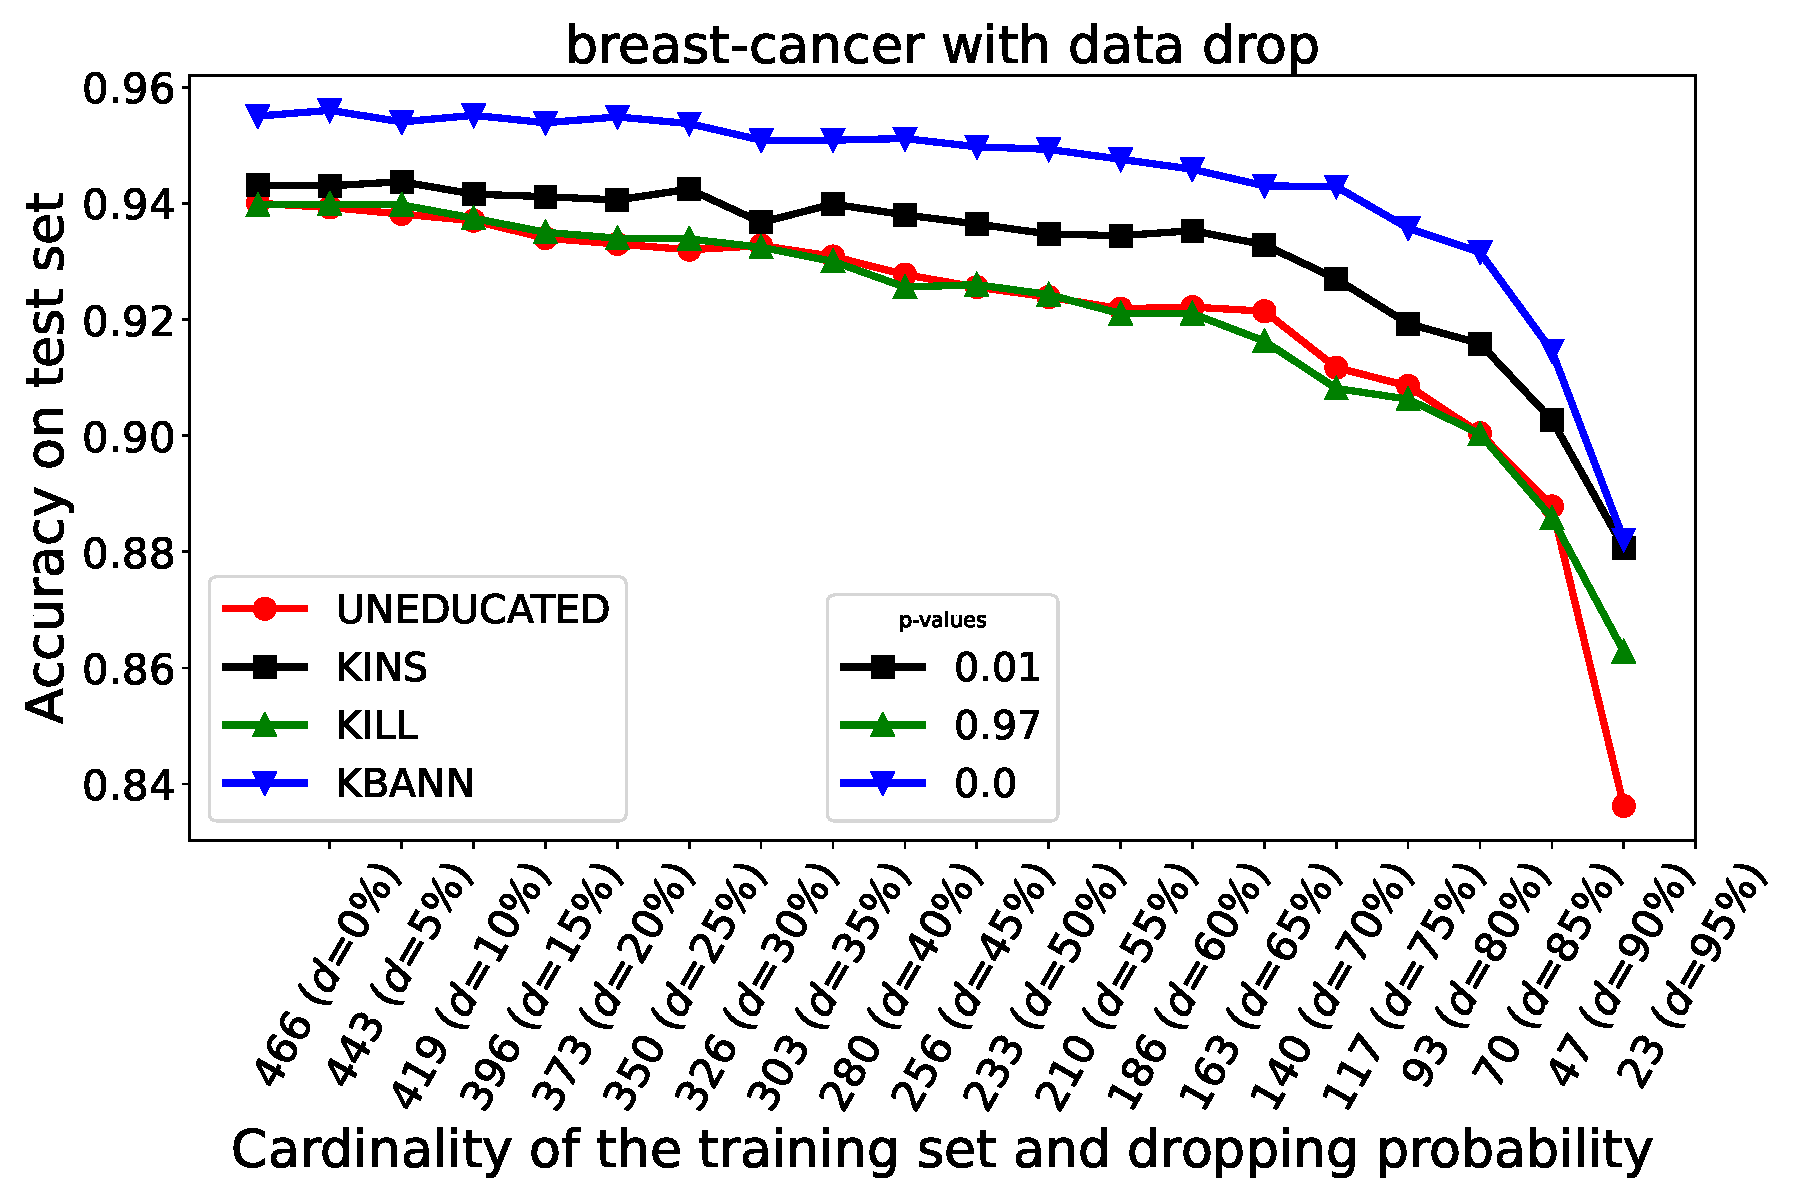
\includegraphics[width=\linewidth]{figures/drop/breast-cancer/uneducated-kins-kill-kbann-accuracy-average-curves}
	\end{subfigure}\hfil
	\begin{subfigure}{\cellsize}
		\caption{}
		\label{fig:psjgs-drop}
		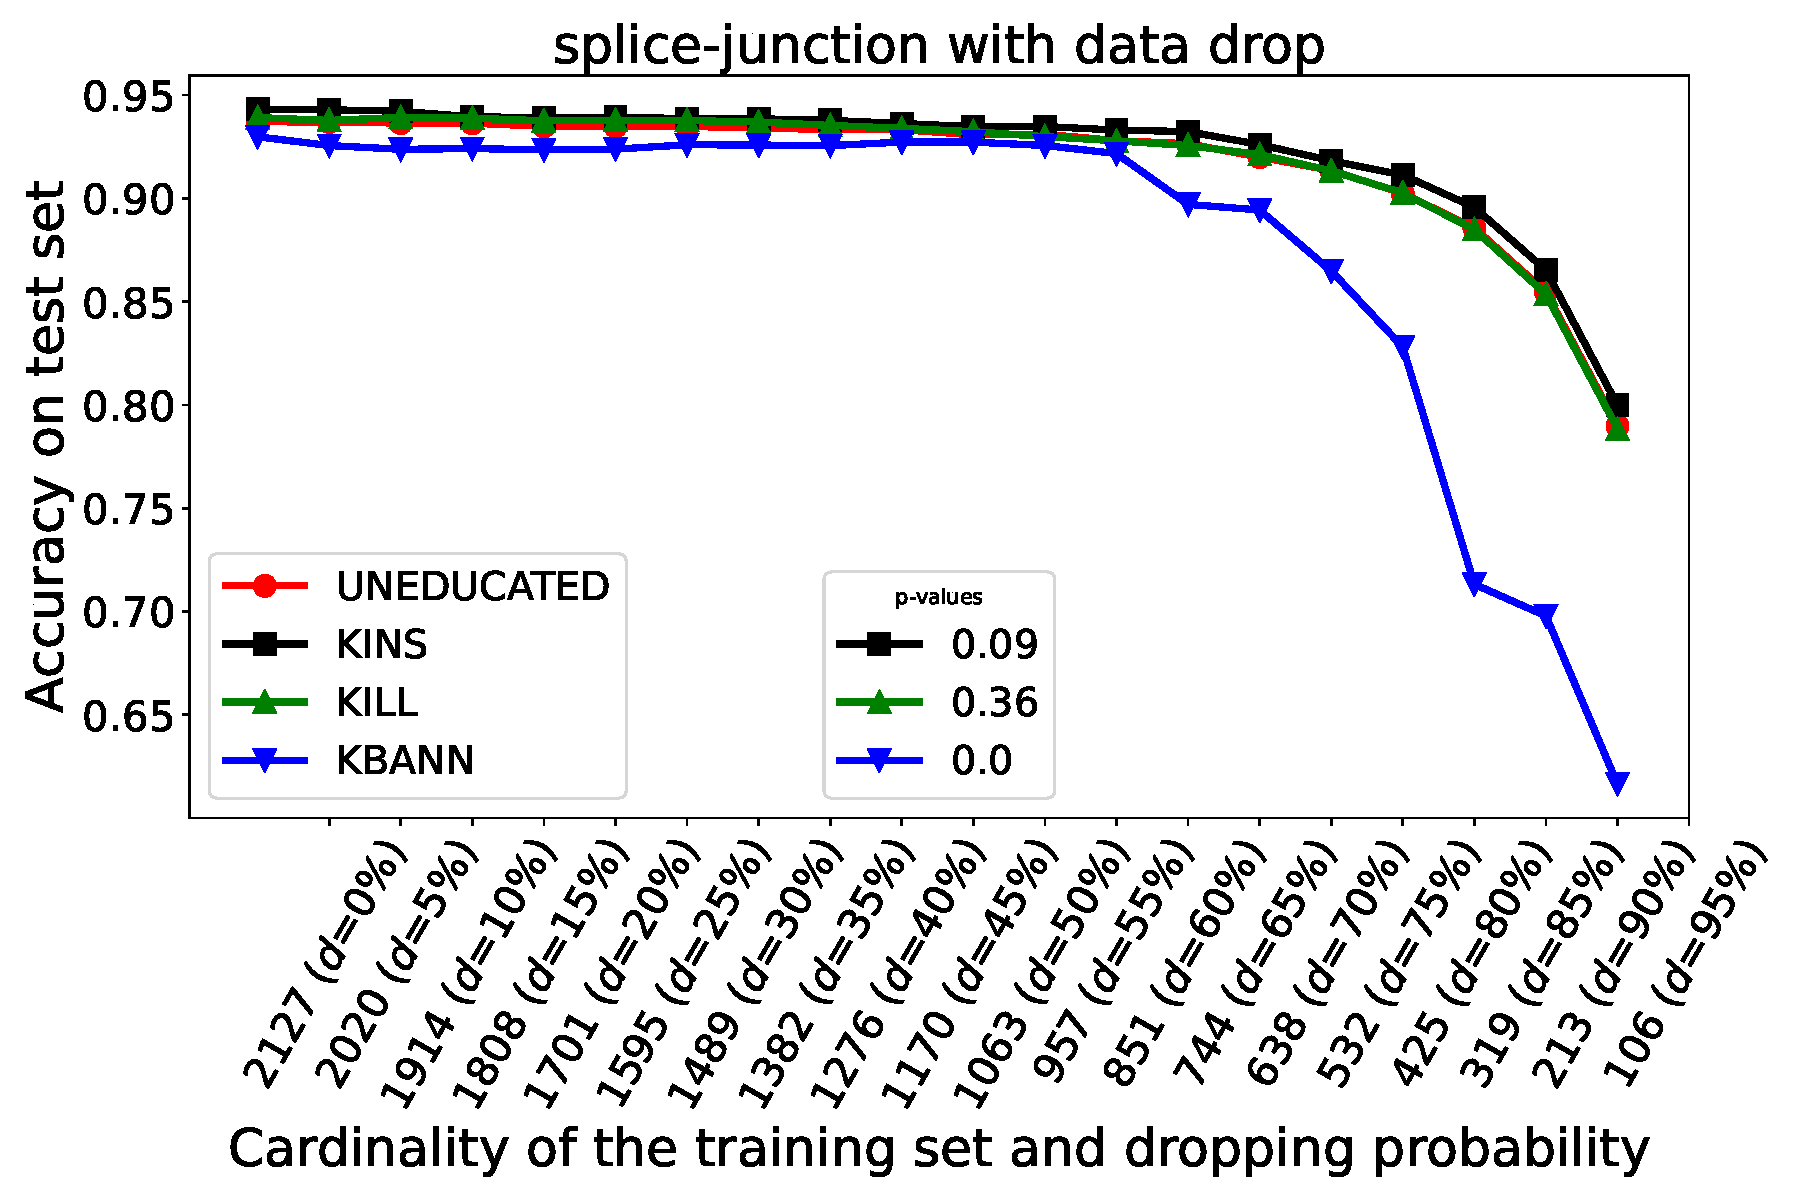
\includegraphics[width=\linewidth]{figures/drop/splice-junction/uneducated-kins-kill-kbann-accuracy-average-curves}
	\end{subfigure}\hfil
	\begin{subfigure}{\cellsize}
		\caption{}
		\label{fig:ci-drop}
		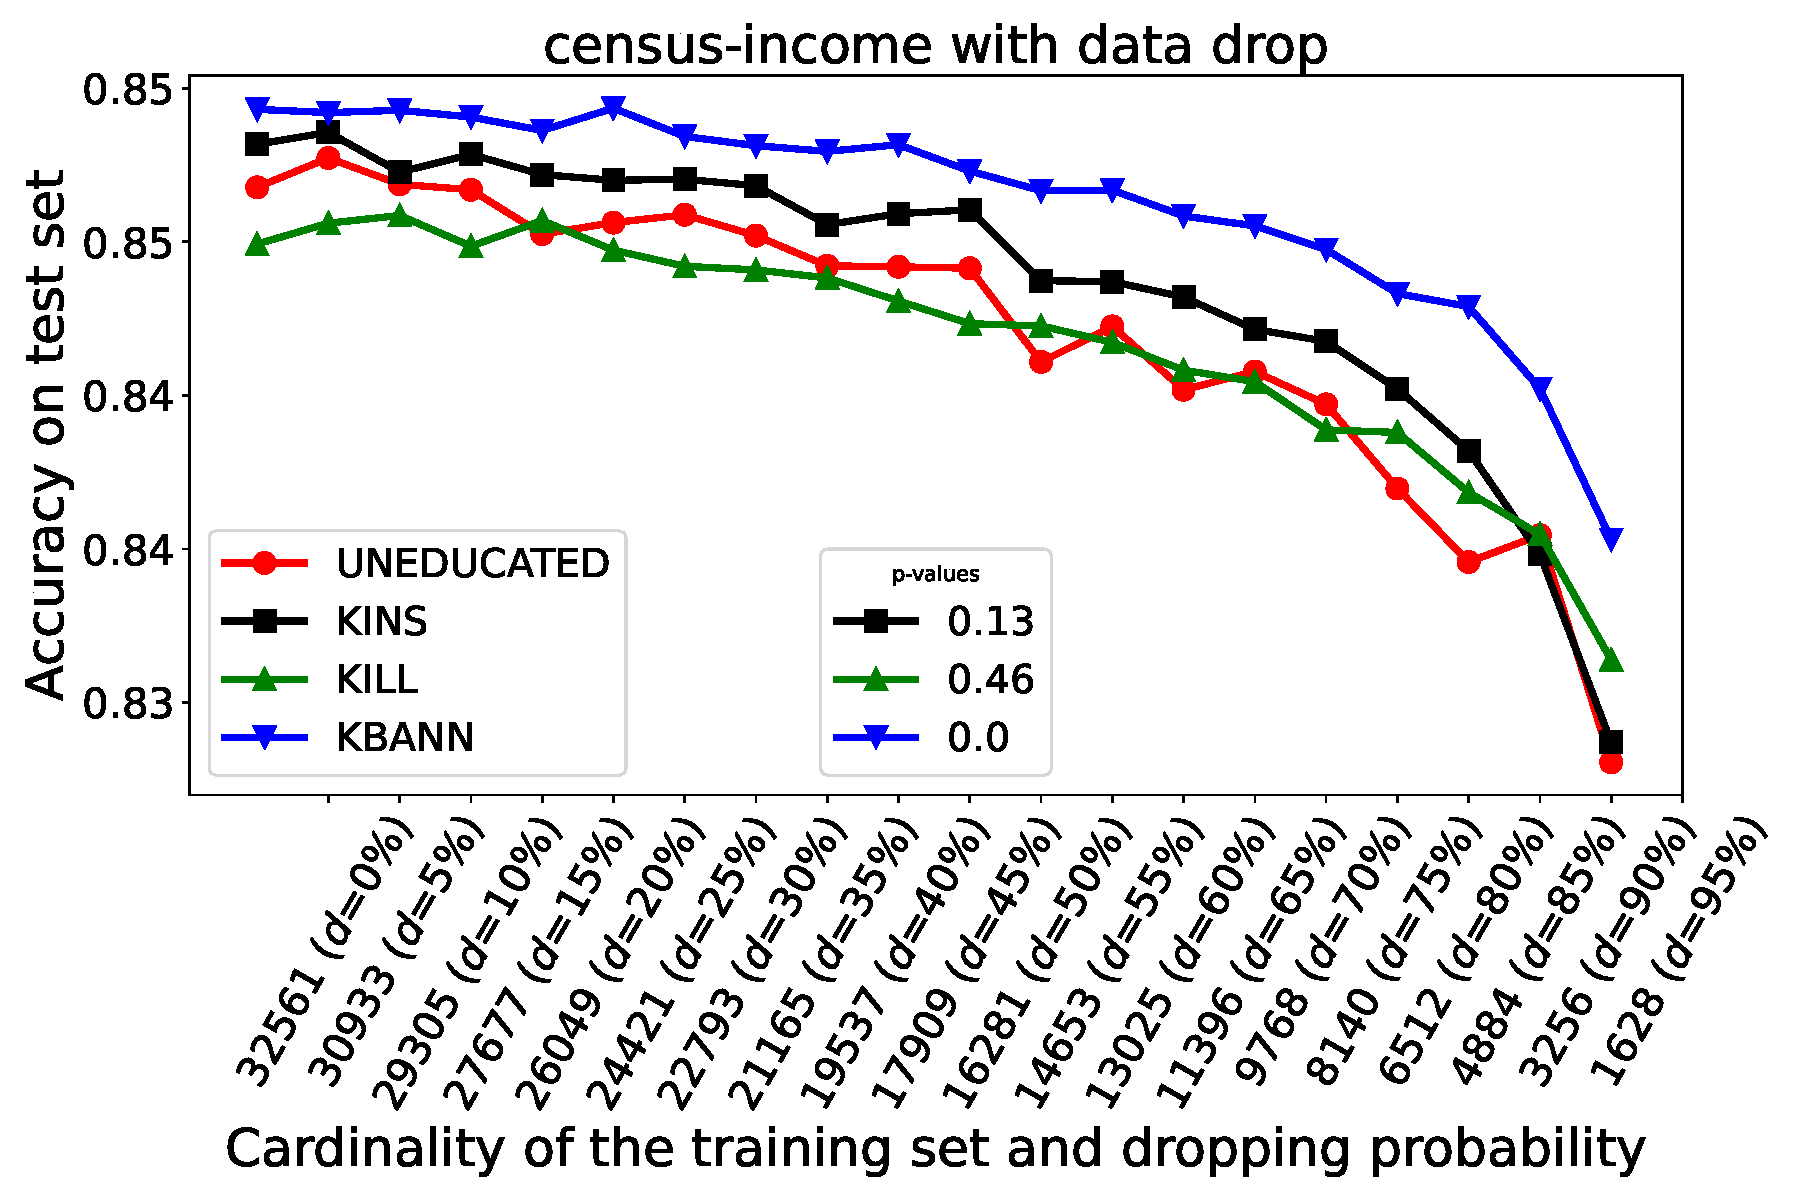
\includegraphics[width=\linewidth]{figures/drop/census-income/uneducated-kins-kill-kbann-accuracy-average-curves}
	\end{subfigure}

	\begin{subfigure}{\cellsize}
		\caption{}
		\label{fig:bcw-noise}
		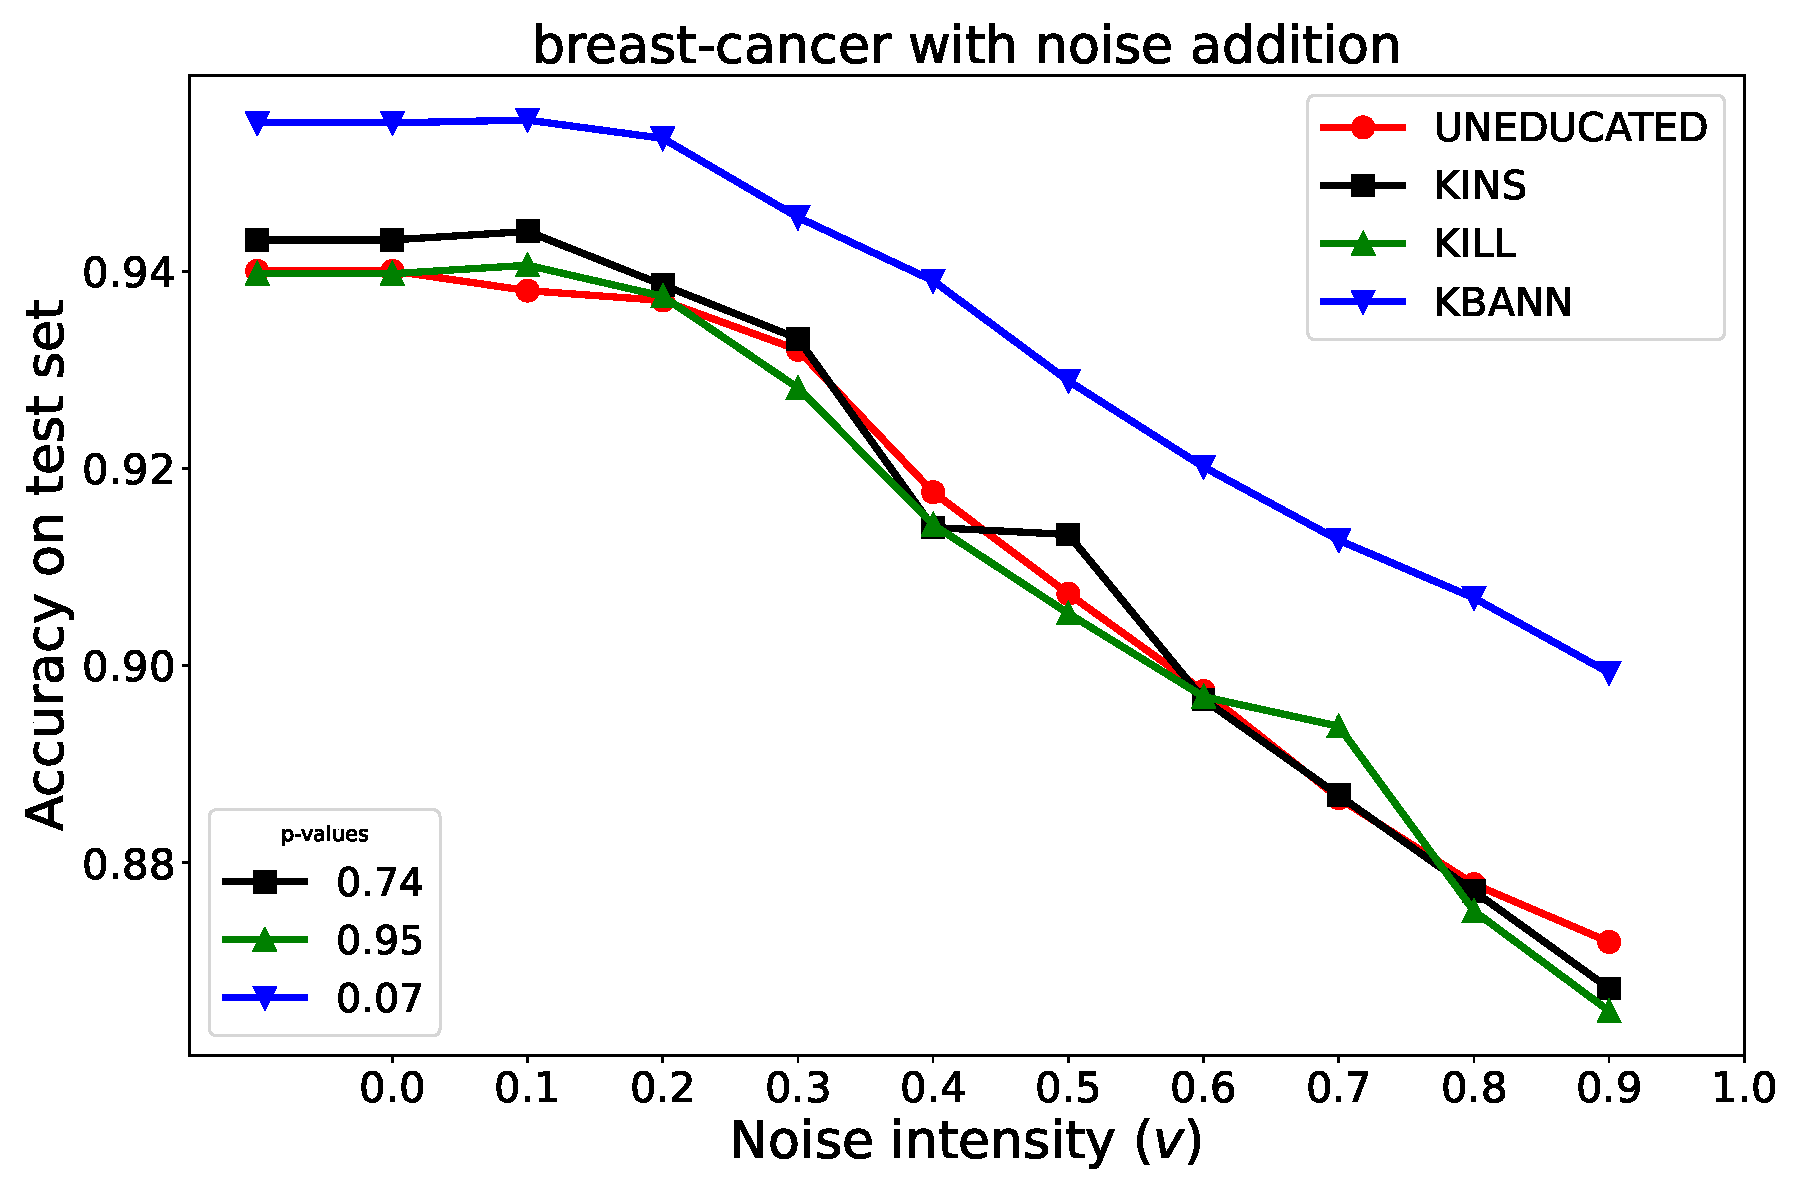
\includegraphics[width=\linewidth]{figures/noise/breast-cancer/uneducated-kins-kill-kbann-accuracy-average-curves}
	\end{subfigure}\hfil
	\begin{subfigure}{\cellsize}
		\caption{}
		\label{fig:psjgs-noise}
		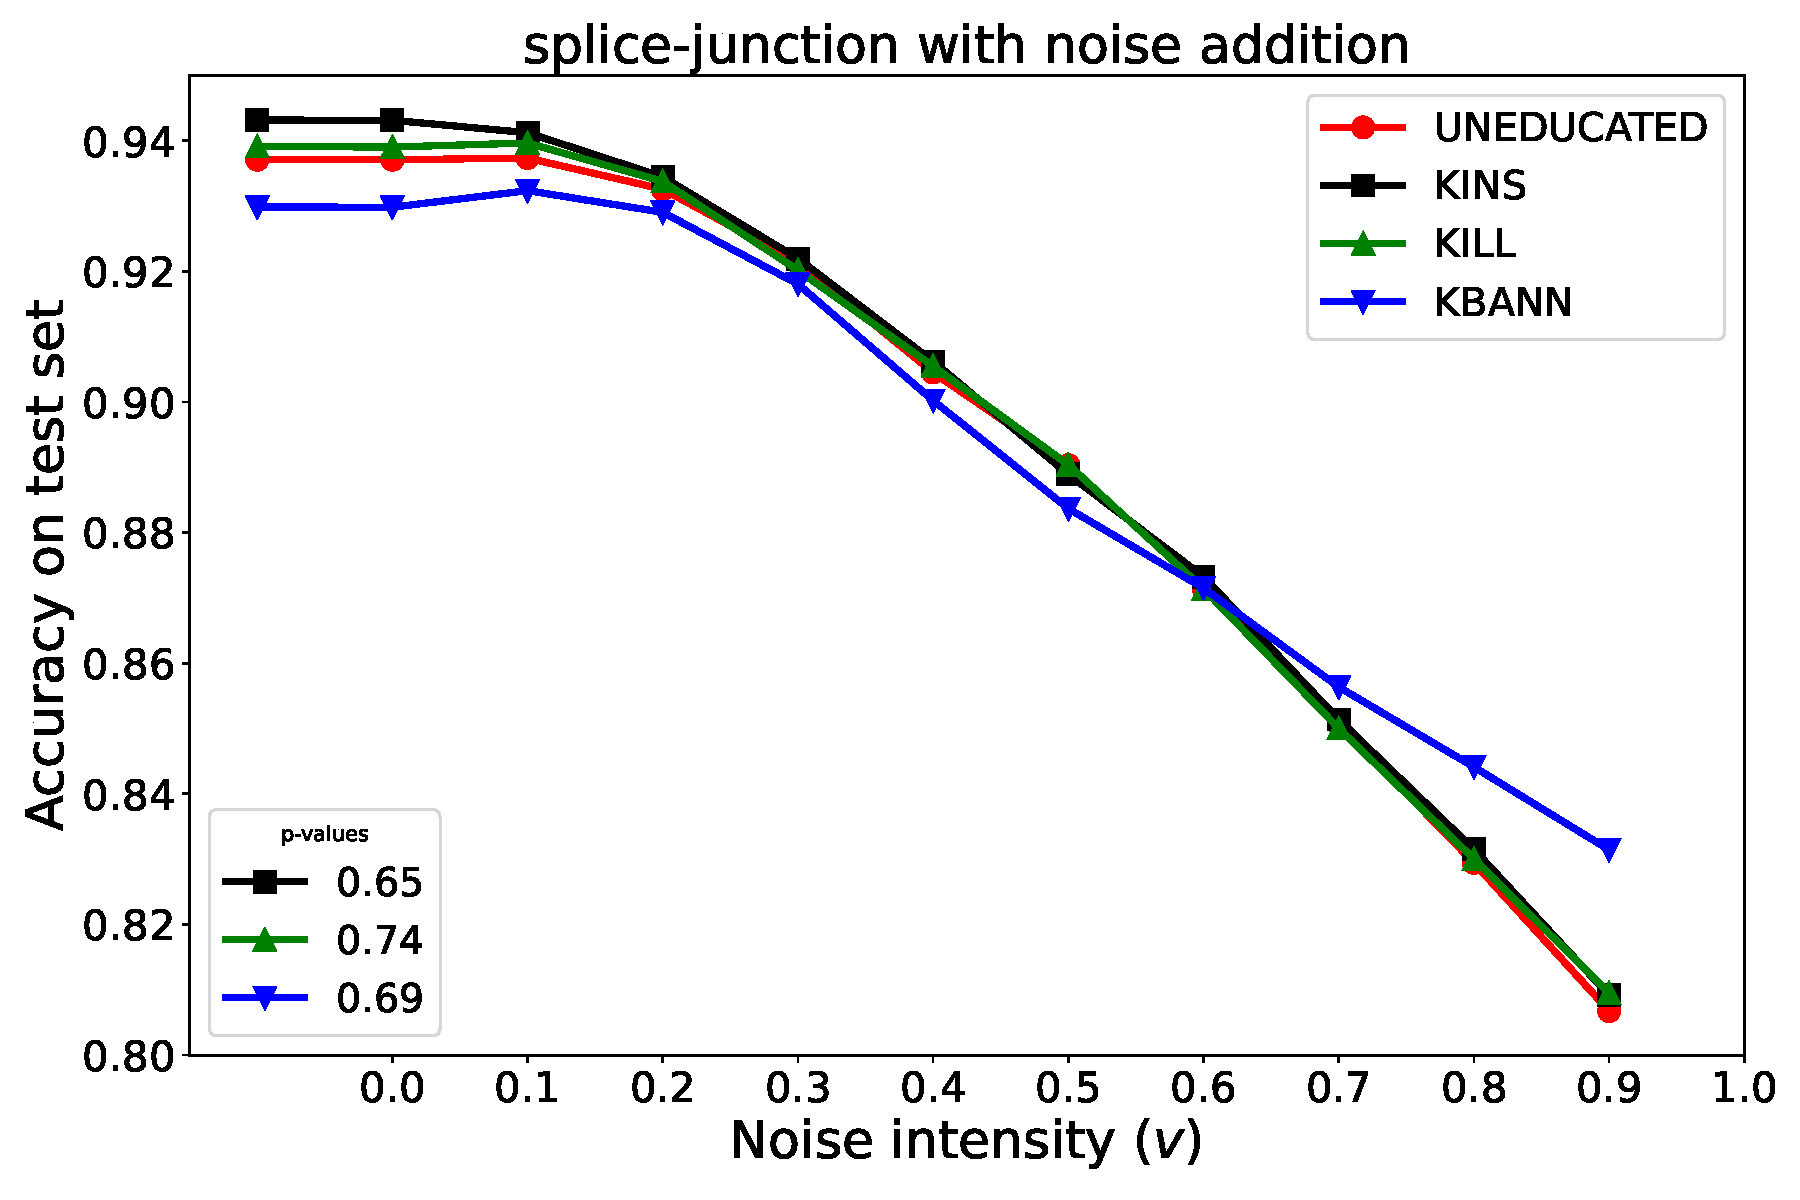
\includegraphics[width=\linewidth]{figures/noise/splice-junction/uneducated-kins-kill-kbann-accuracy-average-curves}
	\end{subfigure}\hfil
	\begin{subfigure}{\cellsize}
		\caption{}
		\label{fig:ci-noise}
		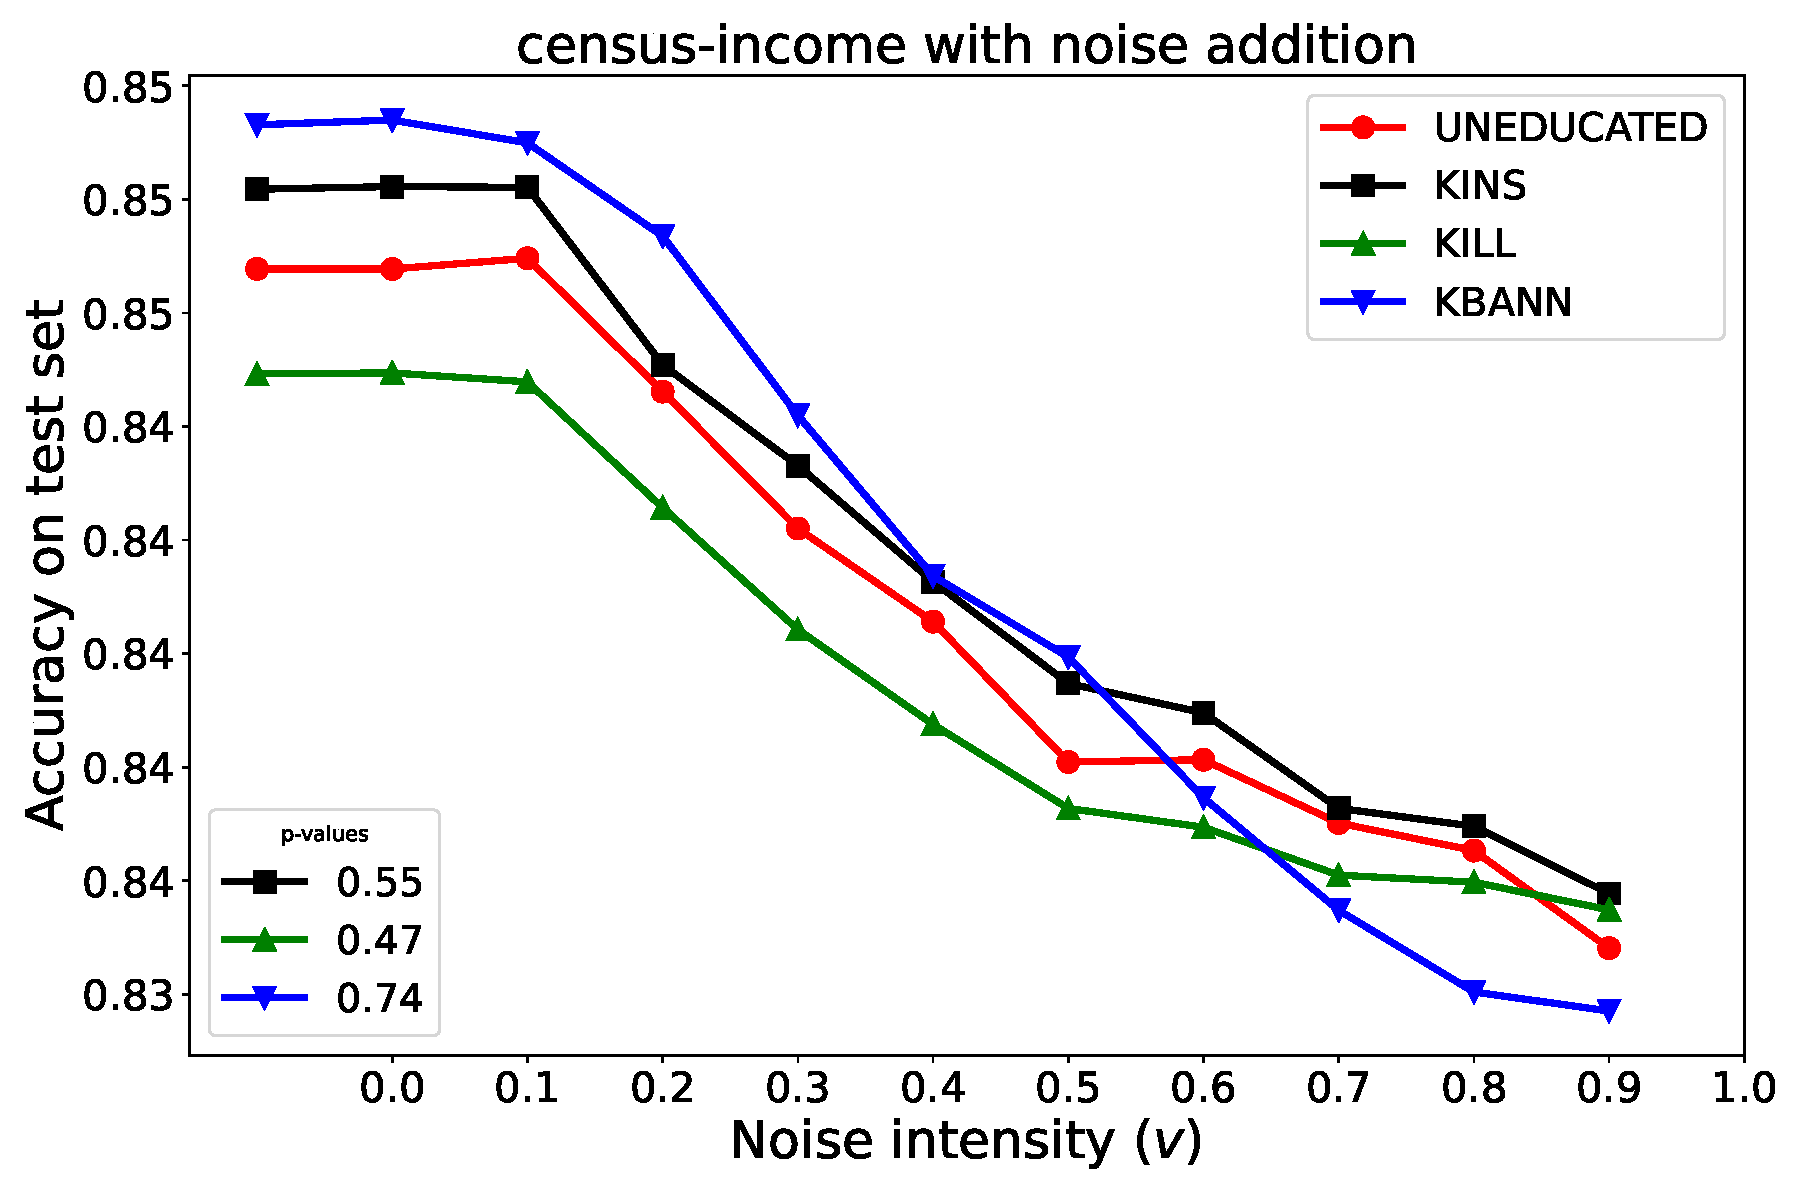
\includegraphics[width=\linewidth]{figures/noise/census-income/uneducated-kins-kill-kbann-accuracy-average-curves}
	\end{subfigure}

	\begin{subfigure}{\cellsize}
		\caption{}
		\label{fig:bcw-label}
		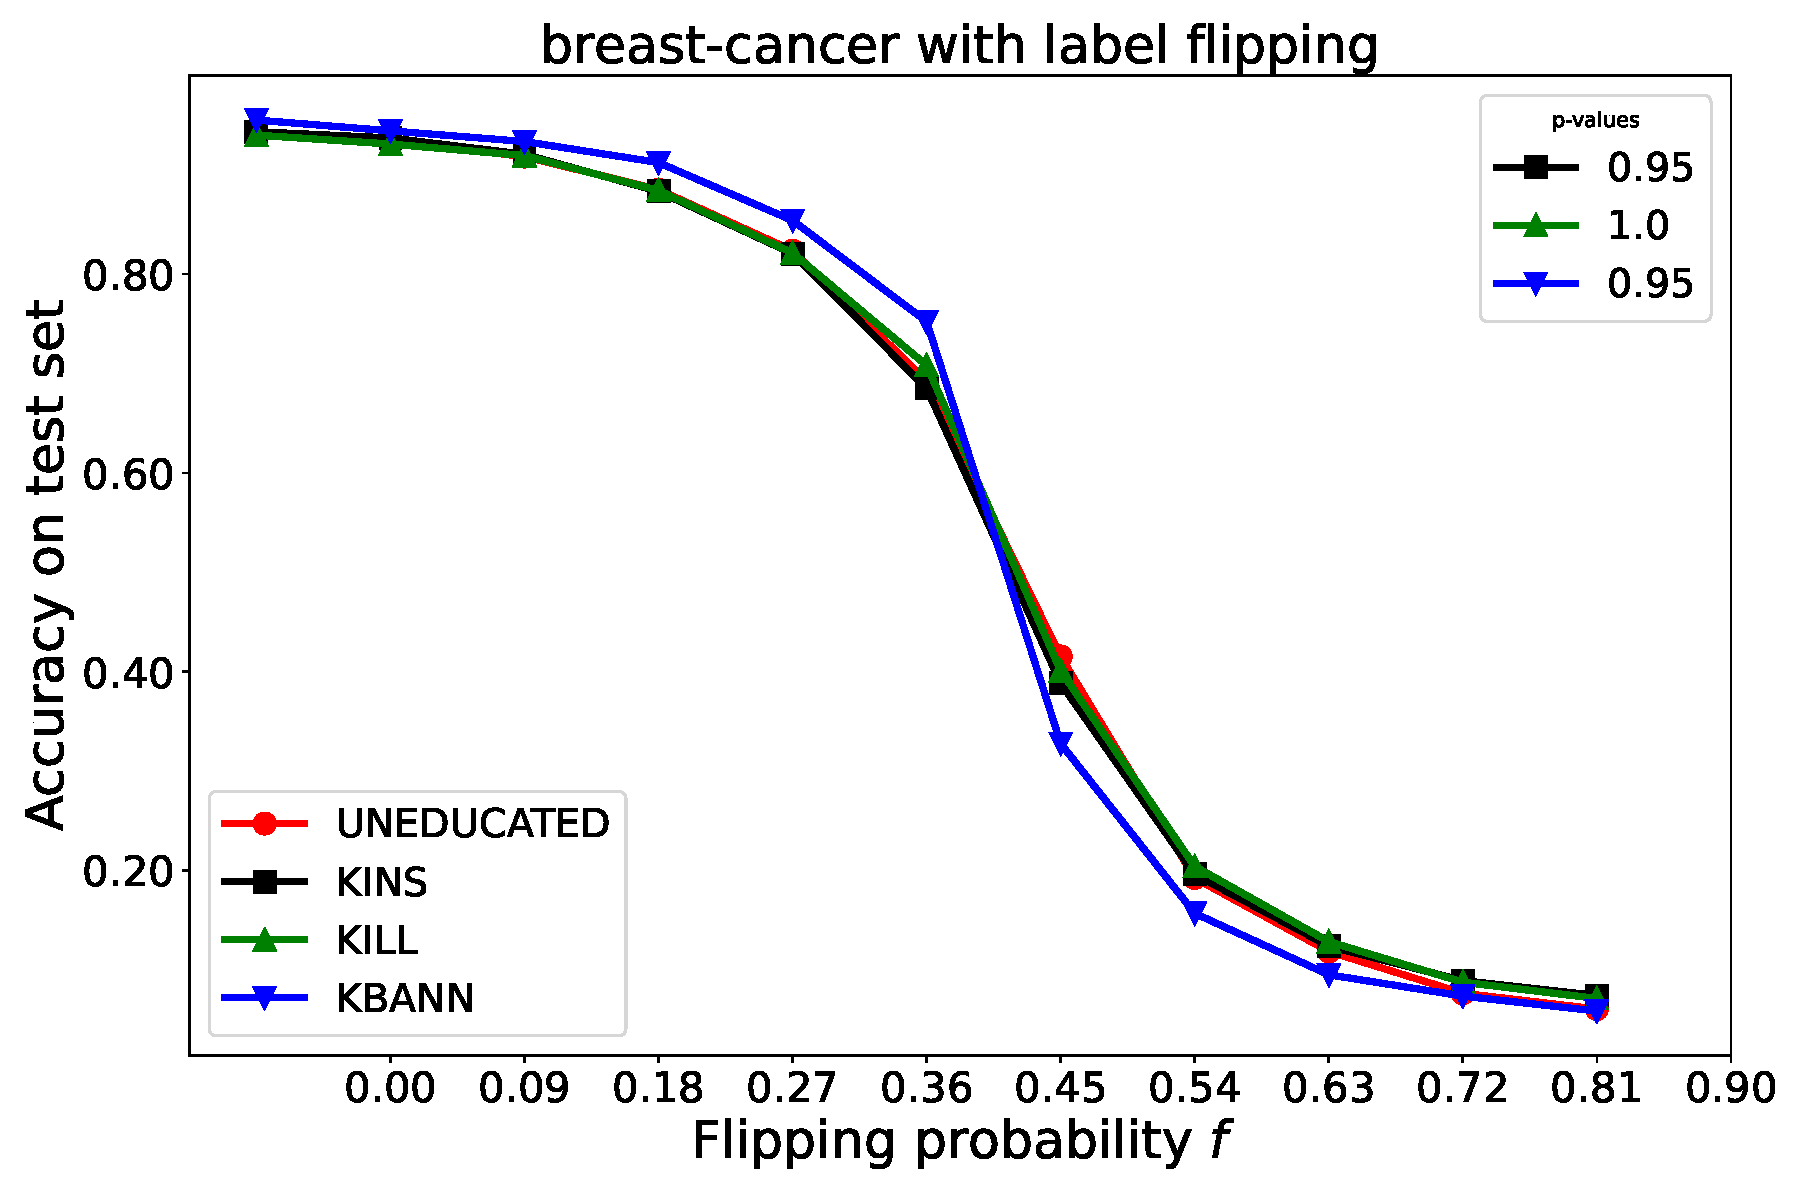
\includegraphics[width=\linewidth]{figures/label_flip/breast-cancer/uneducated-kins-kill-kbann-accuracy-average-curves}
	\end{subfigure}\hfil
	\begin{subfigure}{\cellsize}
		\caption{}
		\label{fig:psjgs-label}
		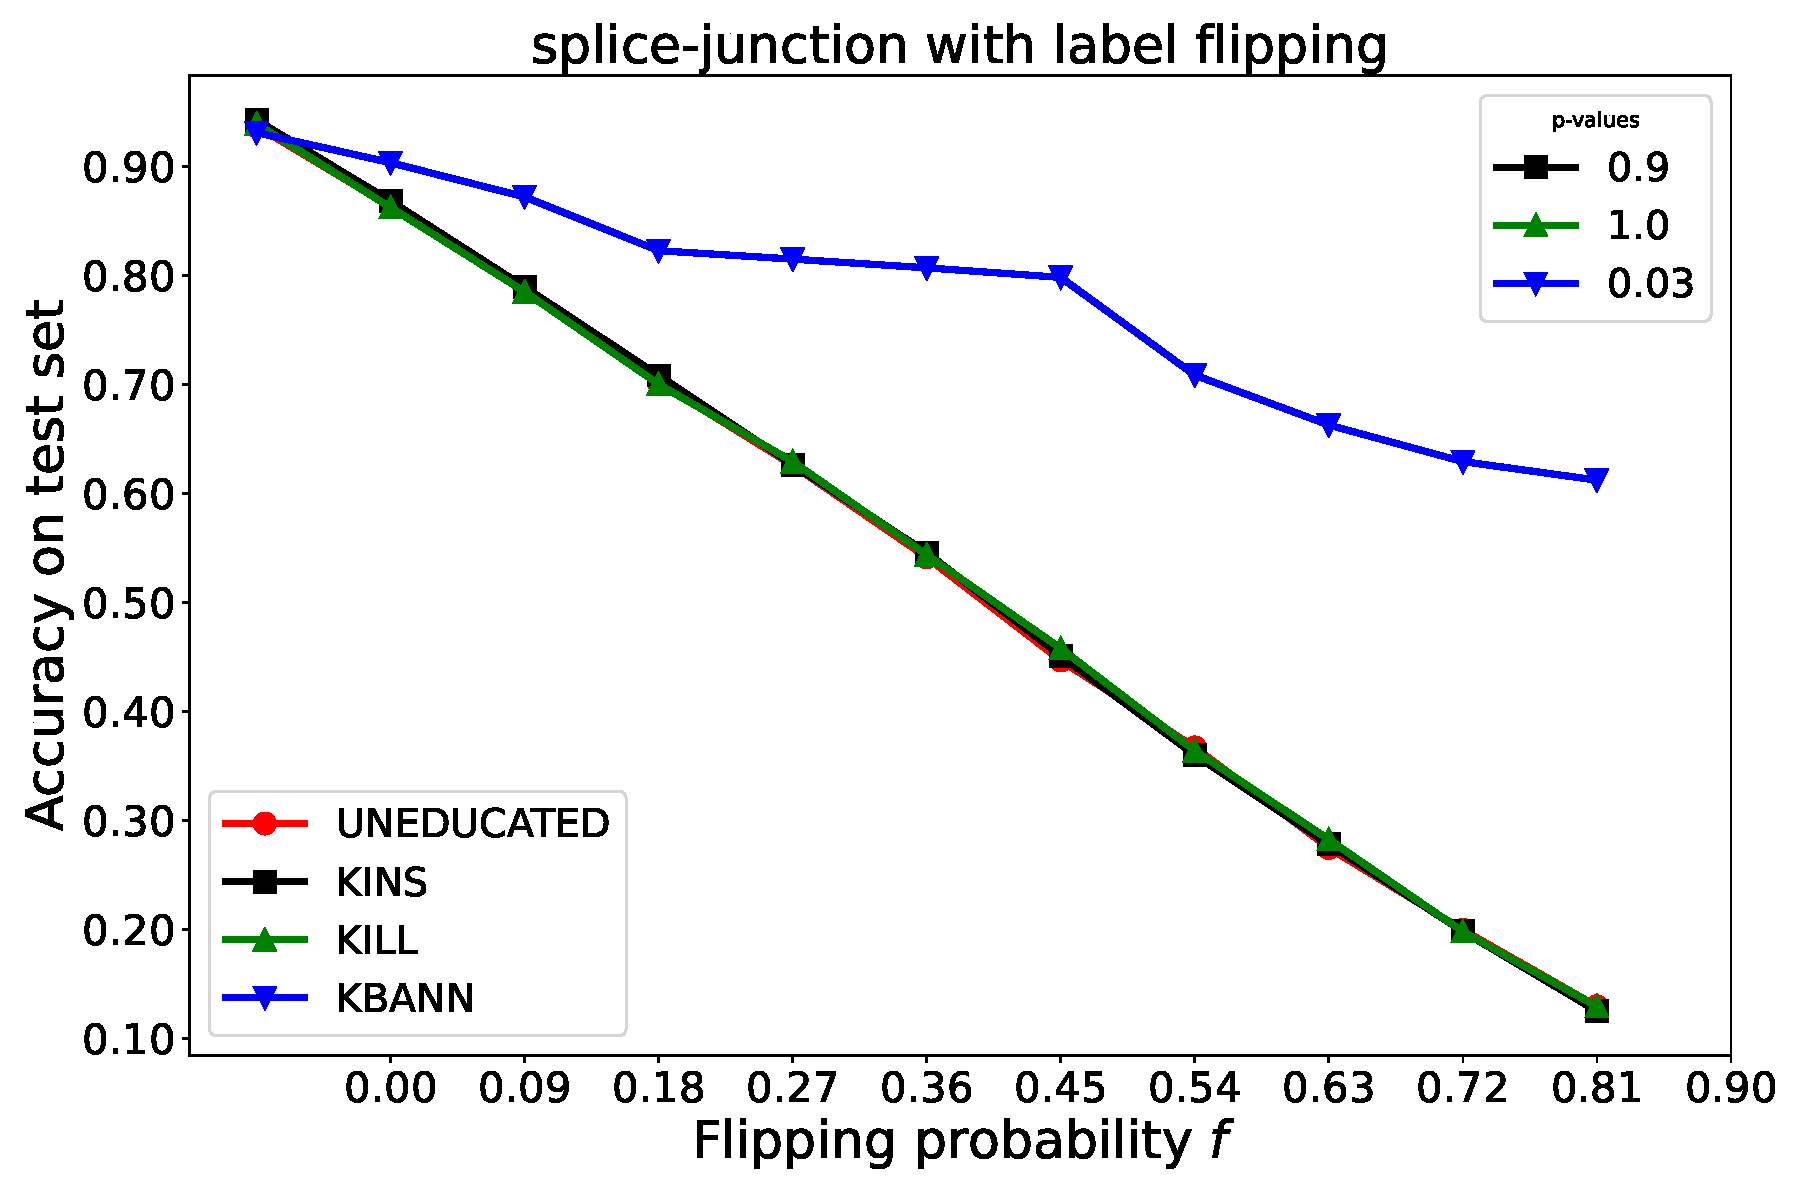
\includegraphics[width=\linewidth]{figures/label_flip/splice-junction/uneducated-kins-kill-kbann-accuracy-average-curves}
	\end{subfigure}\hfil
	\begin{subfigure}{\cellsize}
		\caption{}
		\label{fig:ci-label}
		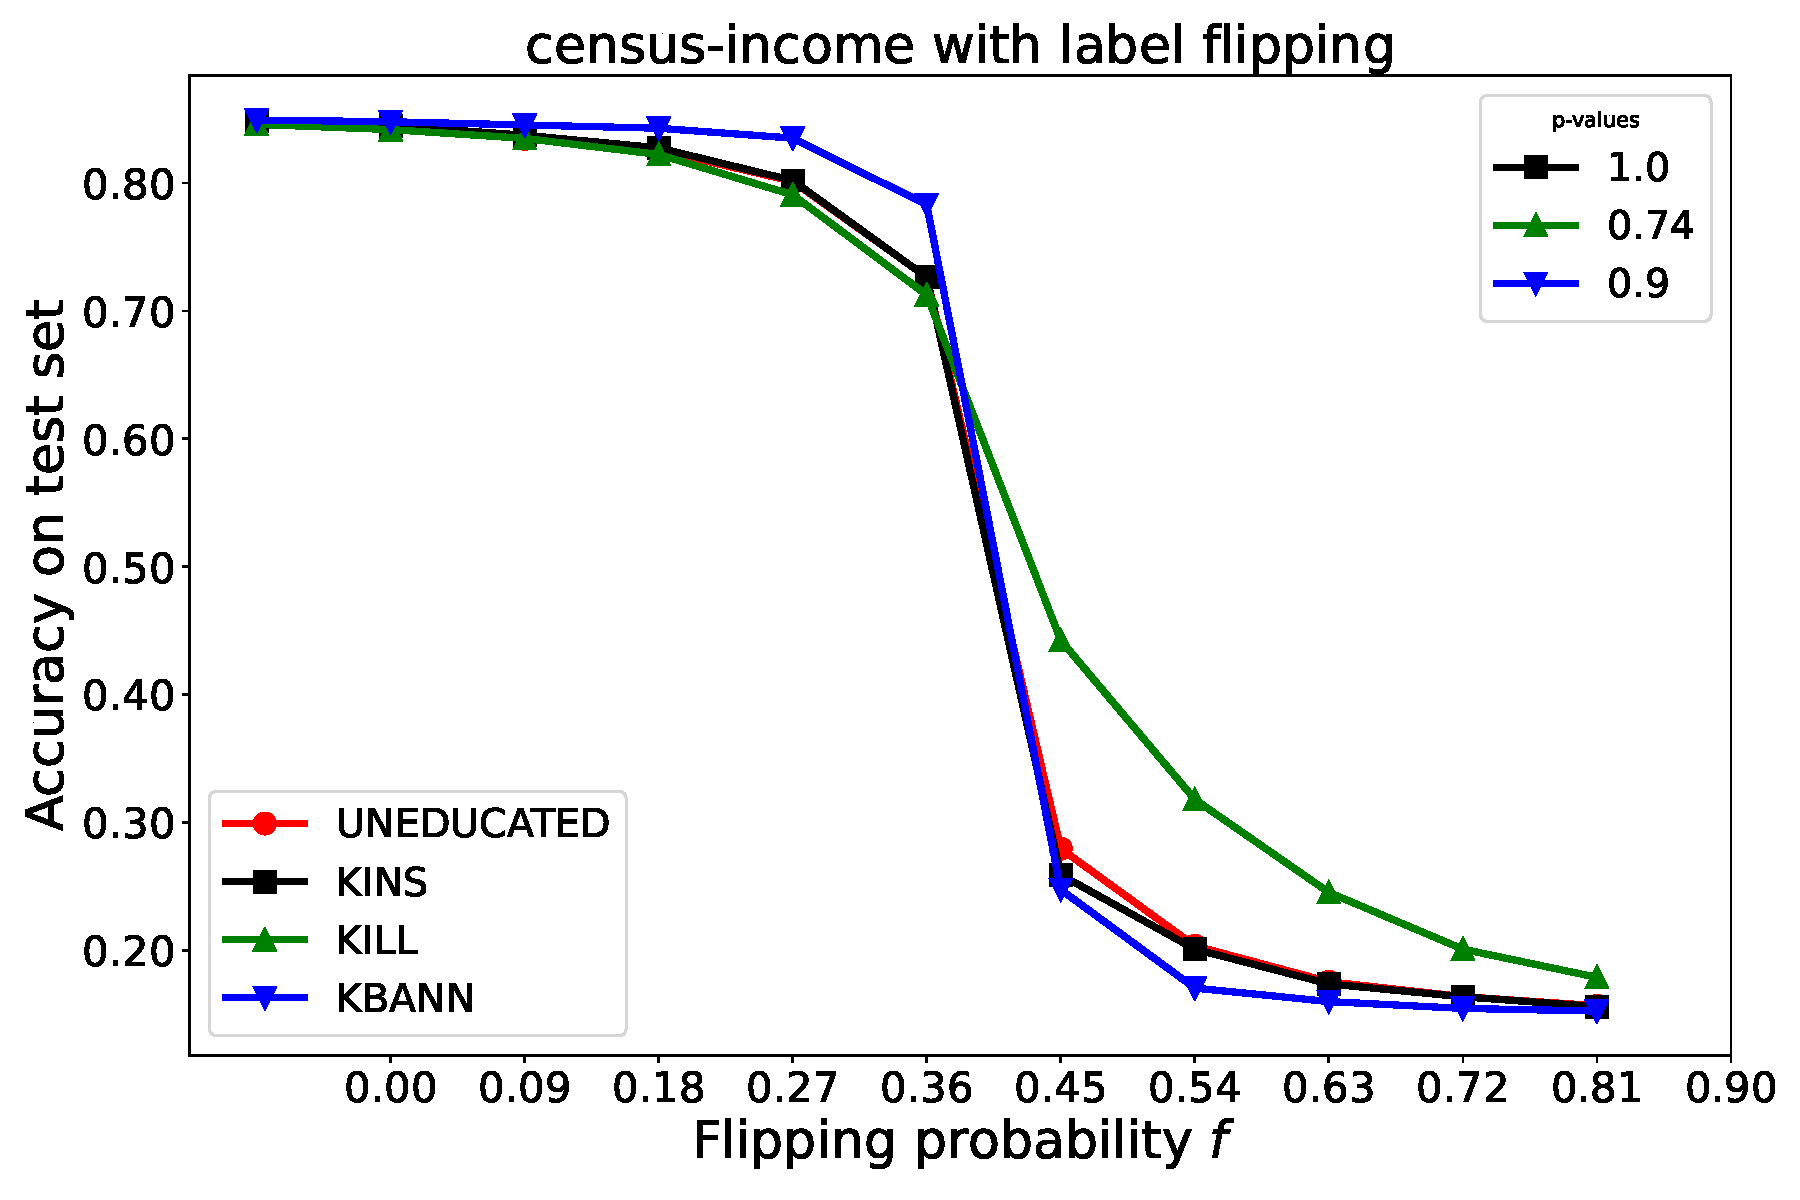
\includegraphics[width=\linewidth]{figures/label_flip/census-income/uneducated-kins-kill-kbann-accuracy-average-curves}
	\end{subfigure}
	\caption{Average accuracy over different datasets with different perturbation strategies}
	\label{fig:accuracy-results}
\end{figure*}
%
\note{TODO: generate again the figures because there is an issue with the x ticks labels}
%
% !TeX root = ../phd-thesis.tex
\begin{table}
    \centering
     \resizebox{\columnwidth}{!}{
         \begin{tabular}{l||rrr|rrr|rrr}
             \toprule
             \multirow{2}{*}{Dataset} &  \multicolumn{3}{c|}{$R_{N, D}(\mathcal{I})$ drop} &  \multicolumn{3}{c|}{$R_{N, D}(\mathcal{I})$ noise} &  \multicolumn{3}{c}{$R_{N, D}(\mathcal{I})$ flip}\\
             \cmidrule{2-10}
             & KINS &  KILL &  KBANN & KINS &  KILL &  KBANN & KINS &  KILL &  KBANN\\
             \midrule
             BCW    & \textbf{1.0493} & \textbf{1.0318} & \textbf{1.0382}  & 0.9960 & 0.9985 & \textbf{1.0109} & 0.9994 & \textbf{1.0184} & 0.9520\\
             PSJGS & \textbf{1.0045} & 0.9968 & 0.8425 & 0.9950 & 0.9984 & \textbf{1.0145} & 0.9962 &  \textbf{1.0026} & \textbf{1.6749} \\
             CI   &  0.9998 & \textbf{1.0039} & \textbf{1.0043} & 0.9992 & \textbf{1.0012} &  0.9965 & 0.9897 & \textbf{1.1703} & 0.9815 \\
             \bottomrule
         \end{tabular}
     }
    \caption[Robustness relative scores for drop, noise and label flip perturbations]{
        %
        Robustness relative scores $R_{N, D}(\mathcal{I})$ for the three perturbation strategies: drop, noise and label flip.
        %
        Bold numbers are the ones greater than 1 (i.e., the educated model is more robust than the uneducated one).
    }
    \label{tab:robustness}
\end{table}


%
This section presents the results of our experiments, focusing on the robustness of educated and uneducated predictors under different perturbation strategies.
%
To compare their performance, we use the Mann-Whitney U Test~\cite{placeholder}, a non-parametric statistical test.
%
A p-value \(\geq 0.05\) indicates no significant difference between the average accuracy distributions, while a p-value \(< 0.05\) suggests otherwise.
%
\paragraph{Data Drop}
%
In the \emph{data drop} experiments (Figure~1a-c), \gls{KBANN} is the only predictor showing significant improvements compared to the uneducated model.
%
It performs better on the \gls{BCW} (Figure~1a) and \gls{CI} (Figure~1c) datasets but exhibits a sharp decline on the \gls{PSJGS} dataset (Figure~1b) when 60\% of the data is removed (\(d = 0.6\)).
%
\gls{KINS} shows slightly better performance than the uneducated model, with a p-value of 0.01 on the \gls{BCW} dataset, indicating significant differences.
%
Overall, educated predictors improve robustness in 6 out of 9 experiments, as shown in Table~1.
%
\paragraph{Noise Addition}
%
The \emph{noise addition} experiments (Figure~1d-f) reveal that \gls{SKI} mechanisms are more sensitive to noise than to missing data.
%
Predictors trained on noisy data show a rapid decline in accuracy, starting early in the perturbation process.
%
\gls{KBANN} outperforms other methods and the uneducated model on the \gls{BCW} dataset (Figure~1d) but performs poorly on the \gls{CI} (Figure~1f) and \gls{PSJGS} (Figure~1e) datasets.
%
Interestingly, \gls{KINS} performs worse than \gls{KBANN}, likely due to its trainable modules being more prone to overfitting noisy data.
%
\gls{KILL} shows similar or worse performance compared to the uneducated model, suggesting that its penalty-based approach does not effectively handle noise perturbations.
%
\paragraph{Label Flipping}
%
In the \emph{label flipping} experiments (Figure~1g-i), predictors exhibit similar behavior on the \gls{BCW} (Figure~1g) and \gls{CI} (Figure~1i) datasets, with no significant differences (p-values close to 1).
%
Performance degrades rapidly when more than 54\% of labels are flipped (\(f = 0.54\)).
%
On the \gls{PSJGS} dataset (Figure~1h), \gls{KBANN} retains nearly 70\% accuracy even at the highest flipping probability (\(f = 0.9\)), outperforming other models, which drop to 20\%.
%
This highlights \gls{KBANN}'s strong adherence to injected knowledge, which mitigates the impact of flipped labels.
%
\gls{KILL} demonstrates good robustness across all datasets, likely due to its loss manipulation strategy, which de-emphasizes corrupted labels during training.
%
\paragraph{Discussion and Take-Home Message}
%
The experiments show that \gls{SKI} methods are most effective in handling missing data, leveraging integrated knowledge to compensate for data scarcity.
%
However, their robustness to noise perturbations is limited, with no significant improvements observed.
%
For label flipping, \gls{KILL} performs well due to its penalty-based approach, while \gls{KBANN} excels on the \gls{PSJGS} dataset due to its strong reliance on injected knowledge.
%
In summary:
%
\begin{enumerate}
    \item \gls{SKI} methods enhance robustness under data scarcity by utilizing integrated knowledge.
    %
    \item Loss-manipulating techniques like \gls{KILL} better tolerate label corruption by reducing the impact of flawed labels.
    %
    \item Structuring-based methods like \gls{KBANN} are more robust than trainable approaches like \gls{KINS}, as they preserve the integrity of injected knowledge.
\end{enumerate}
%
These findings emphasize the importance of selecting appropriate \gls{SKI} methods based on the type of perturbation and dataset characteristics.
\printbibliography[title=References,heading=bibintoc]
\end{refsection}

%----------------------------------------------------------------------------------------
%------------------------------------- PART III -----------------------------------------
%----------------------------------------------------------------------------------------

\part{Engineering of intelligent systems}\label{part:engineering-of-intelligent-systems}

\begin{refsection}
%! Author = matteomagnini
%! Date = 05/03/25

%----------------------------------------------------------------------------------------
\chapter{NeSy AI for real world applications}
\label{ch:nesy-ai-for-real-world-applications}
\minitoc
%----------------------------------------------------------------------------------------

\section{Motivations}\label{sec:nesy-ai-motivations}

\section{Goals and challenges}\label{sec:nesy-ai-goals-and-challenges}

\section{Applications}\label{sec:nesy-ai-applications}

\subsection{\Gls{SKE} for explainable nutritional recommenders}\label{subsec:ske-for-explainable-nutritional-recommenders}

\subsection{A general-purpose protocol for multi-agent based explanations}\label{subsec:a-general-purpose-protocol-for-multi-agent-based-explanations}

\subsection{\Glsentrylong{NeSy} \Gls{AI} for supporting chronic disease diagnosis and monitoring}\label{subsec:nesy-ai-for-supporting-chronic-disease-diagnosis-and-monitoring}

\subsection{\Gls{LLM}-based solutions for healthcare chatbots: a comparative analysis}\label{subsec:llm-based-solutions-for-healthcare-chatbots-a-comparative-analysis}

\subsection{Open-source small language models for personal medical assistant chatbots}\label{subsec:open-source-small-language-models-for-personal-medical-assistant-chatbots}

\subsection{Applying \Gls{RAG} on open \Glspl{LLM} for a medical chatbot supporting hypertensive patients}\label{subsec:applying-rag-on-open-llm-for-a-medical-chatbot-supporting-hypertensive-patients}
%! Author = matteomagnini
%! Date = 05/03/25

%----------------------------------------------------------------------------------------
\chapter{Autonomous learning systems}
\label{ch:autonomous-learning-systems}
\minitoc
%----------------------------------------------------------------------------------------

\section{Motivations}\label{sec:motivations}

\section{Goals and challenges}\label{sec:goals-and-challenges}

\section{Applications}\label{sec:applications}

\subsection{Actively learning ontologies from \Glspl{LLM}}\label{subsec:exact-learning-with-ac{llm}}

\subsection{\Glsentrylongpl{LLM} as oracles for instantiating ontologies with domain-specific knowledge}\label{subsec:llm-as-oracles-for-instantiating-ontologies-with-domain-specific-knowledge}

%! Author = matteomagnini
%! Date = 05/03/25

%----------------------------------------------------------------------------------------
\chapter{Conclusions}
\label{ch:conclusions}
%----------------------------------------------------------------------------------------

\section{Discussion}\label{sec:discussion}

\section{Future work}\label{sec:future-work}
\printbibliography[title=References,heading=bibintoc]
\end{refsection}

\adjustmtc

\end{document}